%%% subaru_ngao_SR_en.tex
% 20120205 iwata subaru_ngao.tex
% 20130310 iwata subaru_ngao_SR_en.tex from subaru_ngao.tex

\documentclass[10pt]{book}
\usepackage{natbib}
\usepackage[sectionbib]{chapterbib}
\usepackage{aas_macros}
\usepackage{graphicx}
%\usepackage[dvipdfm]{hyperref}
\usepackage{color}
\usepackage{lscape}
\usepackage{fancybox}
% fancyhdr package
\usepackage{fancyhdr}
\pagestyle{fancy}
\fancyhf{}
\fancyfoot[C]{\bfseries \thepage}
\fancyhead[LO]{\rightmark}
\fancyhead[RE]{\rightmark}
% PDF toc
%\ifnum 42146=\euc"A4A2
%\AtBeginDvi{\special{pdf:tounicode EUC-UCS2}}\else
%\AtBeginDvi{\special{pdf:tounicode 90ms-RKSJ-UCS2}}\fi


\definecolor{violet}{rgb}{0.4,0.0,0.4}
\definecolor{dblue}{rgb}{0.0,0.0,0.5}
\usepackage[dvipdfmx,%
bookmarks=true,%
bookmarksnumbered=true,%
colorlinks=true,%
pdftitle={Subaru ngAO Study Report},%
pdfauthor={Subaru ngAO Working Group},%
citecolor=dblue,%
linkcolor=dblue,%
urlcolor=dblue,%
]{hyperref}
\citestyle{aa}
\bibliographystyle{apj}

\oddsidemargin   -0.25cm
\evensidemargin  -0.25cm
\topmargin       -0.5cm
\textwidth        16.5cm
\textheight       23.0cm
\parindent        11pt

\def\gsim{\mathrel{\raise0.35ex\hbox{$\scriptstyle >$}\kern-0.6em % Greater/squiggles
\lower0.40ex\hbox{{$\scriptstyle \sim$}}}}
\def\lsim{\mathrel{\raise0.35ex\hbox{$\scriptstyle <$}\kern-0.6em % Less than/squiggles 
\lower0.40ex\hbox{{$\scriptstyle \sim$}}}}

\begin{document}

\title{\Huge Subaru Telescope\\Next-Generation Wide-Field Adaptive
Optics\\Study Report\\(Draft)}
\author{Subaru Next-Generation AO Working Group}
%\begin{titlepage}
\maketitle

%\clearpage
%\input{members}

\tableofcontents

\clearpage
\section*{Acronyms}
%\begin{table}[h]
\begin{tabular}{ll}
AGN & Active Galactic Nucleus \\
AO & Adaptive Optics \\
ASM & Adaptive Secondary Mirror \\
DM & Deformable Mirror \\
ExAO & Extreme Adaptive Optics \\
FoV & Field-of-View \\
FWHM & Full Width at Half Maximum \\
GC & Galactic Center \\
GLAO & Ground-Layer Adaptive Optics \\
HST & Hubble Space Telescope \\
IMF & (Stellar) Initial Mass Function \\
JWST & James Webb Space Telescope \\
LAE & Lyman $\alpha$ Emitter \\
LBG & Lyman Break Galaxy \\
LGS & Laser Guide Star \\
LGSAO188 & Subaru 188-element laser-guide-star adaptive optics system \\
LTAO & Laser Tomography Adaptive Optics \\
MAOS & Multi-Thread Adaptive Optics Simulator \\
MCAO & Multi-Conjugate Adaptive Optics \\
MOAO & Multi-Object Adaptive Optics \\
MOS  & Multi-Object Spectroscopy \\
NBF & Narrow-Band Filter \\
NGS & Natural Guide Star \\
NFIRAOS & Narrow-Field Infrared Adaptive Optics System \\
PSF & Point Spread Function \\
SDSS & Sloan Digital Sky Survey \\
SED & Spectral Energy Distribution \\
SMBH & Super-Massive Black Hole \\
TMT & Thirty-Meter Telescope \\
TTGS & Tip/tilt Guide Star \\
WFE & Wavefront Error \\
WFS & Wavefront Sensor \\
WISH & Wide-field Imaging Surveyor for High-redshift \\
\end{tabular}
%\end{table}
%------------- 
%


%%% Executive Summary
\chapter{Executive Summary
\label{chap:exec_summary}}

\section{Background: Subaru Telescope Future Instrument Plans}

Subaru Telescope Science Advisory Committee (SAC) is an association of 
scientists in universities and institutions in Japan. As a
representative of Japanese optical-infrared astronomical community, they 
have made advisory comments and recommendations to Subaru Telescope,
NAOJ.
In the recommendation report published in March 2009, SAC listed
desirable future instruments of Subaru Telescope. There
are four candidates, namely,

\begin{enumerate}
\setlength{\itemsep}{-3pt}
\item Very Wide-field optical imager (which refers Hyper Suprime-Cam),
\item Wide-field multi-object spectrograph (which refers WFMOS that now
      turns into Prime Focus Spectrograph), 
\item Wide-field near-infrared (NIR) camera, and 
\item NIR integral-field spectrograph.
\end{enumerate}

The third and fourth candidates are NIR instruments. Unlike Hyper
Suprime-Cam and Prime Focus Spectrograph, there has been little activity
on the study of such future NIR instruments for Subaru Telescope.
In response to such recommendation from Japanese community, Subaru
Telescope initiated internal discussions on future instrumentations. 
During the course of such discussions, we recognized the significance of
wide-field adaptive optics system and wide-field NIR instrument
corresponding to such wide-field AO as a strong candidate of the Subaru
future instrument in NIR wavelengths.
Then we have formed the working group for the Subaru next-generation AO
system which consists of scientists not only in Subaru Telescope but
also some members in Japanese universities.

We had the first science workshop for Subaru next-generation AO in
September 2011 in Osaka, and based on science case discussions made
there and technical studies such as AO simulations and conceptual study
of optical design of NIR instrument, we published the study report in
August 2012 (in Japanese). 

This document is an English translation of the executive summary section
of the study report.

\medskip


\section{Subaru Telescope Next-Gen AO System}

There are some different ways to implement Wide-Field AO, and each of
them has its own characteristics (see
Section~\ref{sec:various_ao_systems}). Among them the working group
investigated extensively on two kinds of AO, namely,
{\bf Ground-Layer AO (GLAO)}, and {\bf Multi-Object AO (MOAO)}.

GLAO will achieve seeing improvement over the entire $\phi \gsim 10'$ field
of view (FoV) by correcting only for the disruption of images caused by the
ground layor of the Earth's atmosphere. Although the Strehl ratio with
GLAO should be much less than those by AO systems which achieve
diffraction limited images, you can achieve much wider FoV comparared to
the existing AO systems.

On the other hand, in MOAO, the wavefront errors not over the entire FoV
but toward multiple specific objects within a patrol area are
corrected. 

We made numerical simulations to evaluate performance of these systems
with Subaru Telescope. The details are described in 
Chapter~\ref{chap:simulation}.

\subsection{Ground Layer AO (GLAO)}

Our major findings from simulations for GLAO are as follows. 
Please refer Section~\ref{sec:glao_simulation} for details.

\begin{itemize}
 \setlength{\itemsep}{-3pt}
 \item Under a typical natural seeing condition (FWHM$\sim 0.4''$ in
       $K$-band), GLAO will be able to provide FWHM $\sim 0.2''$ in
       $K$-band. 
 \item Factor 1.5--2 gains are expected on ensquared energy for point
       sources, compared to observations under natural seeing.
 \item Approximately uniform wavefront correction over FoV diameter
       $\sim 20'$ will be achieved. Thus performance of GLAO would not
       be a primary factor in determining the FoV of the system;
       mechanical and optical limitations from the telescope and
       instruments would restrict available FoV.
 \item No significant performance degradation is expected with Tip-Tilt
       guide stars (TTGS) as faint as 18 mag., which is the limiting magnitude
       of the present AO188. Thus it is expected that the sky coverage
       of GLAO would be similar to that of AO188/LGS.
\end{itemize}

Since the fraction of the ground layer among atmospheric turbulence
components is thought to be relatively high in Mauna Kea, Subaru GLAO
could provide good performances. Additionally, we found that on-source
wavefront correction with the adaptive secondary mirror can be higher
than that achieved with the AO188.


\subsection{Multi-Object AO (MOAO)}

Details of simulations for MOAO are described in
Section~\ref{sec:moao_simulation}. Our major findings are as follows:

\begin{itemize}
 \setlength{\itemsep}{-3pt}
 \item If we use 6 GLSs, wavefront correction better than that of GLAO
       system will be achieved for those within a patrol area of a
       radius smaller than $\sim 3'$.

 \item In order to achieve good wavefront error corrections, TTGS should
       be reasonablly close to the target. Consequently, the sky
       coverage to be achieved with MOAO might be fairly similar to the
       FoV of the current AO188.
\end{itemize}

\medskip

Through these studies we have understood expected performances of GLAO 
and MOAO with the Subaru Telescope in reasonably realistic observing
conditions. MOAO will achieve high Strehl ratios for multiple targets,
but for the case with 8m-class telescopes their sky area where MOAO can
perform well will be limited; MOAO should be a strong system if it is
implemented for 30m-class telescopes.
GLAO can, on the other hand, provide seeing-improved wide-field images
which would not be easilly achieved with 30m-class telescopes. It has 
stronger synergy with 30m-class telescopes. We concluded that GLAO
is the primary candidate for the Subaru next-generation AO.

\bigskip

\cornersize{0.25}

\Ovalbox{\parbox{0.95\textwidth}{
\bf GLAO is our primary candidate as Subaru Telescope Next-generation AO
system. It will achieve FWHM $\sim0.2''$ @$K$-band over the entire
$>10'$ field of view, under a typical seeing condition.}}


\section{New Near-Infrared Instrument}

With GLAO we expecte almost uniform seeing improvement for FoV out to
$\sim 20'$. MOIRCS, the current near-IR imaging and multi-object
spectrograph for Subaru Telescope, has FoV of $4' \times 7'$. In order
to fully utilize the capability of GLAO, we definitely need to develop
new wide-field instruments. There are much more challenges in designing 
wide-field near-IR instrument comparared to designing instruments for
optical wavelength; fragile optical components with high throughput in
near-IR, need of cooling to suppress thermal emission, expensive
detectors, and so on. We started optical design studies of the new
wide-field near-IR instrument for the Cassegrain focus of Subaru
Telescope (Section~\ref{sec:inst_optics}).

We found that there is a possible design with a $13'$ diamter FoV for
the case with the same optical design parameters of the secondary
mirror as those of the current infrared secondary mirror. It was also 
found that if we chage the optical parameters of the primary and 
seconday mirrors, we will be able to achieve a $\sim 16'$ diameter
FoV.
There is no such wide-field near-IR instrument than the systems
consiedred here. With the seeing improvement achieved by GLAO, the
instrument should be very unique and competitive.

Although the current optical design is for imager and multi-object
spectrograph (using slit masks), 
from the science case discussions it has been pointed out that the 
Integral-Field Spectroscopy (IFS) is a key function. IFS will enable us
to resolve internal structures of extended objects, and it has become an
indispensable observing method for studying the galaxy evolution.
There are some IFS instruments which can be used with the assistance of
AO, such as VLT/SINFONI, Keck/OSIRIS, and Gemini/NIFS.
The spatial resolution achieved by GLAO should not be as high as those
by current single-conjugate AO systems, simultaneous IFS for multiple
objects in wide FoV can be very unique and strong capability.

We also recognize that GLAO will be able to improve image quality in
optical wavelength ($\lambda > 0.6 \mu$m). Possibilities of new
instruments in optical wavelength would be worth to be
explored. Moreover, the use of adaptive secondary mirror could reduce
the number of optics compared to classical AO systems, and thus thermal
background radiation from telescope and instruments should be
decreased. That would benefit observations in wavelength longer than
2$\mu$m. The adaptive secondary mirror (ASM) would also achieve very
high on-source strehl ratio. ASM / GLAO is not a single instrument but
can be regarded as significant telescope upgrade, and it will open up
various unique opportunities with Subaru Telescope.

\bigskip

\Ovalbox{\parbox{0.95\textwidth}{
\bf We have found an optical design of the Cassegrain instrument with
field-of-view of $13'$--$16'$. The GLAO-assisted wide-field NIR
instrument should have exciting capabilities over existing instruments.
}}


\section{Science with Wide-Field AO and New Instrument}

\subsection{Complete Sensus of the Galaxy Evolution with Large-Scale
  Near-IR Surveys}

Intensive studies of distant galaxies using 8--10m class telescopes, 
4m class survey telescopes as well as space telescopes in the past 15
years have revealed the outline of global history of galaxy formation
and evolution from the early stage of the universe to the present
epoch. We now know that the cosmic star formation rate density or the
average star formation rate for individual galaxies peaked around the
cosmic age of 2--5 billion years ($z\sim1-3$), and since then the global
star formation activity slowly is slowly declining. Stellar mass of
individual galaxies has continuted to grow, and morphologies of giant
galaxies such as spirals and ellipticals have emerged. At the same time,
it has been strongly suggested that super massive black holes which
reside in the center of galaxies have evolved in close connection with
star-formation activities. 
The big questions in the fieldd of galaxy evolution include:
\begin{itemize}
 \item what are the key parameters to drive the galaxy evolution among
       various phenomena that affect star formation activities in the
       galaxies?
 \item what detemines morphologies of the galaxies?
\end{itemize}
Since distant galaxies appear to be small, many of past researches have
been limited to observations of massive galaxies, and especially in many
cases internal structures of such distant galaxies have been neglected. 
Recent development of adaptive optics and sensitive integral field
spectrographs have enabled to resolve those distant galaxies. 

With {\it imaging observations}, we can obtain morphological information
such as size, radial profiles of light sources (stars and ionized gas),
assymetry, and color distribution. From the simulations of imaging
observations with GLAO (Sec.~\ref{sec:gal_sim_imaging}) we found that we
will be able to measure effective radii for less massive galaxies
compared to seeing-limited observations. Measurements of morphological
parameters for huge number of galaxies in various epochs and in wide 
range of mass will enable us to clarify the evolutionary paths of
stellar mass assembly, size, and morphology. We should also emphasize
that we can install new narrow-band filters which are designed to
capture important emission lines at specific redshifts to trace star
formation activities in the multiple galaxies within the target
field. Such addition of new filters and dispersion elements are one
significant advantage of ground-based facilities over the space-bourne
telescopes.

With {\it spectroscopic observations}, abundant physical information
such as star formation rate, amount of dust, metallicity, gas
kinematics, and outflow from galaxies into inter-galactic space. 
Especially, multi-IFS (or slit-scan observations using multi-slit masks)
is an effective way to collect `data cube' (spatial information and
spectral information). IFS studies of distant galaxies were made
primarily for those with the most active star formation at those
epochs, and because only one galaxy can be observed at a time, the
number of sample galaxies are limited (several tens at most). If we
consider the cost of telescope time, significant increase of the number
of sample galaxies through such single-object IFS would not be
expected. Survey using multi-IFS with a wide-field near-infrared 
instrument assisted by GLAO can be a very unique observing capability in
2020s. 
It is well known that the history of galaxy evolution strongly depends
on their environment. Systematics census of of (proto-)clusters of
galaxies including their outskirt is a key observation to understand
environmental effects, and GLAO + wide-field instrument is the best
instrument for such studies. 
The large survey of galaxies at $z\lsim 3$ with Subaru GLAO will produce
the first statistically robust (possibily integral-field) spectroscopic
database of distant galaxy populations.


\subsection{Discovery of the Most Distant Galaxies and Understanding the
  Cosmic Reionization with Narrow-band Imagign Surveys}

Deep observations in near-infrared are challenged by strong OH lines of
the Earth's atmosphere. However, we can suppress background noise for
imaging with narrow-band filters (NBF) which are designed to trace
photons with wavelengths between such strong OH lines. In
Section~\ref{sec:nbf} we discuss the possibility of searching Lyman
$\alpha$ emitting galaxies at $z>7$ with NBFs.
Researches based on the Subaru Telescope's unique capability of
wide-field imaging using the prime focus camera have achieved
discoveries of many of the most distant galaxies. For the redshift of
the current most distant galaxies, however, Lyman $\alpha$ emission is
redshifted to the very end of the wavelength coverage of the optical
instruments. We definitely need sensitive observations in the
near-infrared to push the frontier of the most distant galaxies
further and to understand the process of the cosmic reionization. 

Applications of NBF are not restricted to the search of distant Lyman
$\alpha$ emitting galaxies. Various studies such as systematic survey of
star-forming galaxies with H$\alpha$ emission should have a large
benefit of wide-field near-infrared instrument assisted by GLAO.


\subsection{Observing the Galactic Center}

\begin{itemize}
 \item Imaging and spectroscopy of globular clusters toward the Galactic
       center: kinematics of the Galactic bulge and dark matter
       distribution
 \item Nuclear star clusters as a key population to explore the
       co-evolution of the supermassive black hole and the Galactic bulge
 \item Wide-field astrometry of Hyper-velocity stars around the Galactic
       center
\end{itemize}


\section{Synergy with the Extremely Large Telescopes}

We aim at operation of Subaru GLAO around the end of 2010s and early
2020s. That is the epoch when Extremely Large Telescopes (ELTs) such as
the Thirty Meter Telescope are expected to start their first-light
observations. ELTs will have light collecting power and spatial
resolution substantially superior to the current 8--10m class
telescopes. Observations with ELTs will enable us to explore much
fainter targets, and investigate very details of internal structure of
various objects. On the other hand, wide-field (i.e., FoV larger than
$\gsim10'$) observation with ELTs are extremely challenging. Wide-field
capability of Subaru Telescope has been extended by the telescope
modification and installation of the new prime-focus camera Hyper
Suprime-Cam (1.5 deg. diameter), and the massive fiber-fed spectrograph 
Prime Focus Spectrograph (PFS)\footnote{The spectral coverage of PFS is
0.38$\mu$m -- 1.3$\mu$m.} is under development.
To implement observational capability which cannot be achieved by ELTs
and to execute observations complimentary to those by ELTs should be key
strategies for 8--10m class telescope in 2020s and later. 
A combination of Subaru GLAO and wide-field near-IR instruments is one
of the most significant projects which further develop the uniqueness
and advantage of Subaru Telescope and feed astronomical targets to ELTs
for detailed characterizations.

\bigskip

\Ovalbox{\parbox{0.95\textwidth}{
\bf Wide-field instruments for survey are key instruments in the era of
TMT and other ELTs. Subaru Telescope should work in cooperation with TMT
and be complimentary to the TMT's capabilities. The Development of a
wide-field near-infrared instrument is essentially important for Subaru
Telescope.}}


\section{Development Plan}

%$B3+H/7W2h$K$D$$$F$O(BChapter~\ref{chap:dev_plan}$B$K$F5-=R$7$F$$$k!#(B

\subsection{Development Organization and Funding}

\begin{itemize}
 \item Core group: next-generation AO study working group (Subaru
       Telescope AO team + scientists in Subaru and universities in
       Japan)
 \item Subaru Telescope staff + NAOJ (Mitaka) staff + international
       partnership
 \item Fund-raising from external competitive grants from the Japanese 
       government 
 \item NAOJ budget for Subaru Telescope modifications should be
       considered. 
 \item International partnerships are essentially important for both
       human resources and fudning.
\end{itemize}

\subsection{Development Schedule}

In order to maximize scientific outcomes, it is important to develop
the wide-field instrument with GLAO prior to the science observations of
TMTs, to execute survey observations, and to construct list of target
objects for detailed studies with TMT. We should construct a development
plan to start science observation by 2020.



%%% Science
\chapter{Science with ULTIMATE-SUBARU 
\label{chap:science}}

In this chapter we introduce science cases proposed to be carried out
with Subaru Telescope Next-Generation AO (ngAO) and clarify
specifications ngAO and associated new instruments should satisfy.

The GLAO system we are studying have following features (see
Chapter~\ref{chap:system_design} for details):

\begin{itemize}
\item Wide-field seeing improvement by correcting WFE caused by ground
      layer of the Earth's atmosphere. Seeing improvement will provide
      not only better angular resolution, but also the significant
      improvement of sensitivity especially for point-like sources. On
      the other hand, the WFE correction (and subsequently angular
      resolution) for individual sources are not as good as classical AO
      systems (such as AO188 of Subaru) which are designed to achieve
      diffraction-limited image for narrow-field. 
\item Number of optical component should be reduced by using the
      Adaptive Secondary Mirror. This means that thermal emission from
      telescope and instrument should be reduced, and that sensitivity
      at longer wavelength ($\gsim 2\mu$m) will be improved.
\end{itemize}

We have developed studies of the science cases under the recognition of
these features, and with strong interactions with technical studies of
the GLAO system and the associated instruments.

We have two primary scientific objectives (or 'Science Drivers') of this
project. The one is `Complete Sensus of Galaxy Evolution with
Large-Scale Near-IR Surveys', and the other is `Discovery of the Most
Distant Galaxies and Understanding of the Process of the Cosmic
Reionization'.

Because GLAO can provide images with better spatial resolution and
improved sensitivity, the GLAO system can be a `significant upgrade
of Subaru Telescope' rather than an introduction of a new
instrument. Various reseaches should be benefitted with the system.
In Septermber 2011 we had a science workshop in the Japanese community
titled `Science Workshop for Subaru Telescope Next-Gen AO System' in
Osaka,
Japan\footnote{\href{http://www.naoj.org/Projects/newdev/ws11b/index.html}{http://www.naoj.org/Projects/newdev/ws11b/}}. 
We also had 'Subaru GLAO Science Workshop' in June 2013 in Hokkaido
Univ. Some Canadian researchers as well as those from Taiwan has
participated the workshop and presented their prospects. 
Through these workshops, we received important suggestions and proposals
for wide-range of researches, such as galaxy evolution, growth of
massive black holes, galaxy archaeology, the Galactic center,
star-forming regions, and exoplanets. From this science workshop we
started more extensive discussions on various science cases, and this
chapter represents the current outcomes of such discussions and studies.

\def\thisdir{science/veryhighz/}


\section{Search for Galaxies at $z>7$ with Narrow-Band Imaging
\label{sec:nbf}}

\noindent
\begin{center}
%% Authors
{\bf Ikuru Iwata$^{1}$}\\
$^1$ Subaru Telescope, National Astronomical Observatory of Japan, 650
North Aohoku Place, Hilo, HI 96720, USA
\end{center}
\vspace{0.5cm}

\subsection{Introduction}

Subaru has been one of leading facilities pushing the frontier of
the distant universe. A unique capability of the prime focus camera
(Suprime-Cam) have enabled us to conduct wide-field survey which is
essentially important to find very rare objects such as luminous distant
galaxies. One of the efficient methods to find distant star-forming
galaxies is to detect Ly$\alpha$ emission using narrow-band filter (NBF) 
imaging. A strongly star-forming object with a redshift 
$z = \lambda_\mathrm{NBF} / \lambda_\mathrm{Ly\alpha} -1$ could
appear to be bright compared to those with adjacent broad-band
filters. Galaxies detected with this methods are called as 'Ly$\alpha$
emitters (or LAEs)'. The current most distant galaxy with a spectroscopic 
confirmation is an LAE at $z=7.215$, which was discovered by
\citet{Shibuya2012} using Suprime-Cam with a narrow-band filter NB1006
(central $\lambda$ is 10,052\AA).

Currently a new prime focus camera for Subaru Telescope in optical
wavelength, Hyper Suprime-Cam (HSC), is under testing. HSC has more than
seven times wider field-of-view, and it is expected to enable us
conducting deep surveys much more efficiently than the current
Suprime-Cam. HSC will have a NBF called NB101 which has a central
$\lambda$ is 10,095\AA, which will be used to detect many $z\sim 7.3$
LAEs. 
However, the wavelength of the redshifted Ly$\alpha$ is almost at the
long wavelength limit of the CCDs, and finding galaxies at $z>7.5$ with
cameras with CCDs is impossible. So deep near-IR surveys are mandatory
to push the redshift frontier further.

(Cosmic reionization)


\subsection{Surveys with ULTIMATE-SUBARU}

We will use special narrow-band filters which are designed to trace
photons with wavelength ranges between the strong OH air glows from the
Earth's atmosphere.
Here we assume three wavelength ranges as a fiducial set to study the
feasibility.

\begin{table}[!ht]
\begin{center}
\begin{tabular}{rrr}
\hline
$\lambda_\mathrm{c}$ & FWHM & $z_{\mathrm Ly\alpha}$\\
\hline
1.0625 & 0.015  &  7.74\\
1.340  & 0.019  & 10.0 \\
1.550  & 0.022  & 11.75\\
\hline
\end{tabular}
\end{center}
\caption{
Central wavelengths ($\lambda_\mathrm{c}$ in $\mu$m), FWHM (in $\mu$m),
 and redshifts of Ly$\alpha$ emission at $\lambda_\mathrm{c}$ for NBFs
 considered here.
}
\label{tab:iwata_nbf_setup}
\end{table}

\begin{figure}[!ht]
\centerline{
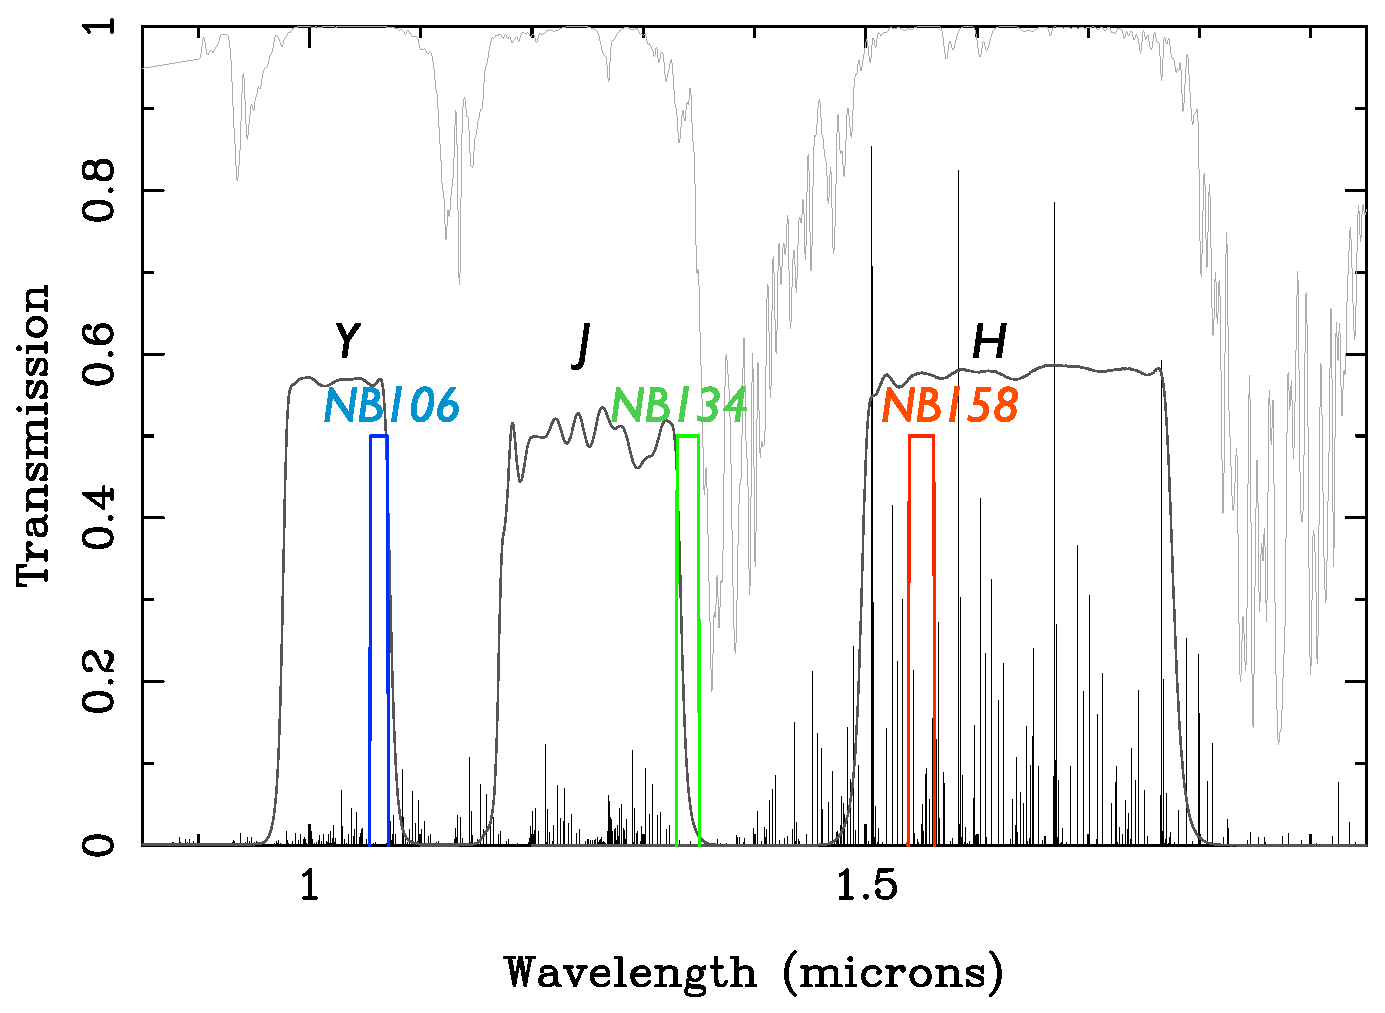
\includegraphics[width=80mm]{\thisdir figs/iwata_pg_filters_nbf01vd.eps}
}
\caption{
Transmission curves of NBFs considered. Transmission curves for $Y$,
 $J$, $H$-bands and the atomospheric transmission, and OH air glow
 strength (in arbitrary unit) are also shown.
}
\label{fig:iwata_filter_nbf}
\end{figure}

\par\noindent
[Very narrow band width filters]


\par\noindent
[What should be clarified with ULTIMATE-SUBARU.]

\subsection{Proposed Observations}

\par\noindent
[Target objects: sample selection, number of objects, number of observing
fields, sky area.]

\par\noindent
[Observing modes: imaging or spectroscopy.]

\par\noindent
[Required observing time:]

\par\noindent
[Special requirements for ULTIMATE-SUBARU other than baseline
specifications, if any.]

\subsection{Synergy and Competitions}

\subsubsection{Synergy with TMT}

\subsubsection{Competitions with other facilities}

Instruments for 8--10m class telescopes.

ELT instruments.

Space-based projects.

\bibliographystyle{apj}
\bibliography{\thisdir nbf}

%%% 20131217 iwata adopt to report form
\def\thisdir{science/hizpeak/}

%\documentclass[]{article}
%\usepackage{graphicx}
%\usepackage{amsmath,amssymb}
%\usepackage{natbib,aas_macros}
%\citestyle{aa}
%\bibliographystyle{apj}


%\oddsidemargin   -0.2cm
%\evensidemargin  -0.2cm
%\topmargin       -0.2cm
%\textwidth        16.5cm
%\textheight       22.0cm
%\parindent        11pt

\newcommand\lya{Ly$\alpha$}
\newcommand\ha{H$\alpha$}
\newcommand\hb{H$\beta$}
\newcommand\paa{Pa$\alpha$}
\newcommand\oii{[O~{\sc ii}]}
\newcommand\oiii{[O~{\sc iii}]}
\newcommand\nii{[N~{\sc ii}]}

\def\gsim{\mathrel{\raise0.35ex\hbox{$\scriptstyle >$}\kern-0.6em % Greater/squiggles
\lower0.40ex\hbox{{$\scriptstyle \sim$}}}}
\def\lsim{\mathrel{\raise0.35ex\hbox{$\scriptstyle <$}\kern-0.6em % Less than/squiggles 
\lower0.40ex\hbox{{$\scriptstyle \sim$}}}}
\def\msun{{\rm M}$_{\odot}$}

%\begin{document}
%\noindent
%\Large
\section{Galaxy Formation at Its Peak Epoch Revealed by ULTIMATE-Subaru
 Project \label{sec:highzpeak}}

\noindent
%\\vspace{5mm}
%\large
\begin{center}
%% Authors
{\bf Tadayuki Kodama (NAOJ), Yusei Koyama (NAOJ), Ken-ichi Tadaki (NAOJ),
and Michael Balogh (Univ. of Waterloo, Canada)}
\end{center}
\vspace{0.5cm}

\normalsize
%%      Introduction (summary of past researches, key questions)
\subsection{Introduction}
\subsubsection{The peak epoch of galaxy formation}

Recent observations have established that star-formation (SF) and AGN
activities come to peaks at $1\lsim z\lsim 3$ (cosmic look-back time of 8--11 Gyrs)
\citep[e.g.,][]{madau96,lilly96,hopkins06}.
This means that the bulk of stellar contents within
present-day galaxies were formed in that peak epoch of cosmic SF
history. It is therefore crucial to study these rapidly growing
galaxies at this peak epoch, in order to fully
understand the key physical drivers of galaxy formation and evolution.

One of the important discoveries in the recent extra-galactic
astronomy is the tight relationship between galaxy stellar mass and
star-formation rate (SFR), which is often referred to as the ``star
formation main sequence'' \citep[e.g.,][]{Brinchmann04, elbaz07, daddi07}.
The SF main sequence is now investigated out
to $z\gsim 2$ \citep[e.g.,][]{whitaker12}, and it is shown that the
SFR of $z\sim 2$ galaxies (for a given stellar mass) is $\sim$30 times
higher than those in the present-day universe. It is reported that the
scatter around the SF main sequence is relatively small at all redshifts
($\sim$0.2--0.3~dex), which implies that galaxy stellar mass is an
important parameter regulating SF activity of galaxies.

However, the scatter around the main sequence reflects the variation
of gas accretion history of galaxies, hence it is important to
identify the origin of the scatter and understand the key parameter
that makes the strongest impact on the gas accretion history of
galaxies. \citet{wuyts11} studied how the galaxy structure and the
mode of SF activity depend on the position on the SFR--mass diagram.
They find that the upper envelope of SF main sequence is dominated by
dusty (i.e.\ high SFR$_{\rm IR}$/SFR$_{\rm UV}$ ratio) galaxies (Fig. 2)
with high sersic index ({\it n}) (Fig.\ 1), suggesting a rapid build-up
of mass in the nuclear regions of these systems, due for example to
galaxy-galaxy interactions/mergers \citep{wuyts11}.
This kind of studies---linking {\it global} and {\it internal} properties
of galaxies---will become more and more important for understanding 
``how galaxies grow'' in the early universe (see also Section~*1.2*).

Another important parameter that drives galaxy evolution is
``environment''. It is well established that galaxy properties are
strongly dependent on environment, known as the morphology--density,
color--density, or SFR--density relations in the local universe 
\citep[e.g.,][]{dressler1980, lewis2002, gomez2003}.
Recent 
observational studies have shown that the environment strongly affects
the ``fraction'' of red/quenched galaxies, while the environmental
effect seems to be milder for SF activities {\it amongst} SF galaxies
\citep{balogh2004,peng2010}. A more recent study by \citet{koyama13b}
extend this idea up to $z\sim 2$ by comparing
H$\alpha$-selected galaxies in clusters and field environments
\citep[Fig.3,][]{koyama13b}.
These studies suggest that the environmental effect instantly shut down SF
activity of galaxies once the truncation process is started
so that they do not appear as ``being-truncated'' galaxies and do not change
the location of the main sequence of {\it star-forming} galaxies.

\subsubsection{Internal structures of forming galaxies}

The high-resolution imaging by $Hubble\ Space\ Telescope$ (HST) allows
us to study evolution of galaxy morphologies in distant universe.
For galaxies at $z>1.5$, near-infrared (NIR) observations are essential 
to sample the rest-frame optical lights, tracing the distribution of stellar mass. 
NIR high-resolution imagings have shown that massive quiescent galaxies 
at $z\sim2$ tend to be extremely compact compared to local ones with 
the same stellar mass \citep[e.g.,][]{vandokkum08}, suggesting 
the inside-out scenario; dense core are first formed by dissipational processes 
such as gas rich mergers and outer parts are subsequently built up by 
dry minor mergers \citep[e.g.,][]{vandokkum10}. 
However, \citet{vandokkum13} 
investigate the evolution of surface density profiles for Milky-Way-like
galaxies from $z=2.5$ to $z=0$ and find that bulges form in lockstep
with disks to $z\sim1$. This result rules out the inside-out 
growth for less massive Milky-Way-like galaxies and needs some sort of
physical mechanisms such as bar instabilities or clump migration to
explain the simultaneous formation of bulges and disks.

Star-forming galaxies at the peak epoch of galaxy formation actually tend 
to have irregular, clumpy morphologies unlike the present-day galaxies 
on the Hubble sequence \citep{elmegreen05}. Although such 
clumpy structures are often seen in both rest-frame UV and optical
wavelengths \citep{guo12}, the kinematics of ionized gas show ordinary
disks with symmetric rotation of $v_\mathrm{rot}\sim200-300$ km s$^{-1}$ 
\citep{genzel06}. Many of them also exhibit large local velocity
dispersions of $\sigma=30-90$ km s$^{-1}$, suggesting that the gas disks
commonly have random motions.

In the past several years, the efficient gas supply through cold streams along 
filamentary structures is suggested to be a preferred mechanism to account for 
enhancement in SFRs, clumpy structures embedded in ordinary rotational disks, 
and large velocity dispersions \citep{dekel09}.
The steady, narrow, cold gas streams penetrate the shock-heated media of 
massive dark matter haloes and continuously supply a large amount of gas 
to the inner regions of star-forming galaxies. The smooth streams maintain 
dense gas-rich disks, as observed in CO observations \citep{tacconi10}.
In such a gas rich disk, a small gas perturbation in the radial direction would 
grow up and fragment into giant clumps by a gravitational instability.
Then, the internal gravitational interactions within a perturbed disk generate
turbulences and the velocity dispersion becomes progressively larger. 
Though any direct observational evidence for cold gas streams has not been 
found yet, this may account for all the differences in the properties between 
high-$z$ and local galaxies.

The clumpy structures of galaxies suggest a new scenario of bulge formation. 
In the numerical simulations, clumps formed from gravitational instabilities can 
migrate toward a galaxy center as a result of their mutual interactions and of 
dynamical friction against the host disk, and coalesce into a young bulge 
\citep[e.g.,][]{inoue12}.
This is an unusually efficient process to carry a large amount of gas and 
star from galactic disks to bulge components. Then, a starburst would be 
induced at the center by a collision between the clumps in a manner similar 
to a major merger \citep{barnes96}. However, we have very little 
knowledge about it observationally.

\subsubsection{Mahalo-Subaru Survey Project}

In order to explore this critical epoch for galaxy formation,
near-infrared (NIR) observations are essential,
as the rest-frame optical light, where most of the information
on stellar populations exist, is all redshifted into NIR regime. 
However large systematic observations at NIR which achieve both depth
and width have been limited due to high background noise (including the
forest of OH sky lines) in the ground-based NIR observations and limited
field of view of NIR instruments on large telescopes. 
The situation is dramatically improving recently because of the advent
of various wide-field imagers and spectrographs on 8--10m telescopes. 
MOIRCS and FMOS on Subaru are the first examples, and MOSFIRE on Keck,
HAWK-I/KMOS on VLT, and FLAMINGOS-2 on Gemini are bursting out
recently. 

By utilizing the large field of view of MOIRCS (4$'$$\times$7$'$), 
we firstly conducted deep and wide NIR imaging of 4 promising
proto-clusters at 2$\lsim$$z$$\lsim$3 \citep{kodama07}.
Based on the $J-K_s$ vs $K_s$ colour-magnitude diagrams, we revealed
that the red sequence of cluster galaxies at the massive-end above
10$^{11}$\msun are just emerging between $z=3$ and 2, indicating that we
are entering the epoch of massive galaxies formation in proto-clusters.  
We have also been conducting the ``Mahalo-Subaru'' project 
\citep[MApping HAlpha and Lines of Oxygen with Subaru;][]{kodama13}, 
in which we targeted proto-clusters at 1.45$<$$z$$<$2.53 
\citep{hayashi10, hayashi11, hayashi12, tadaki12, koyama13a},
%(Hayashi et al. 2010; 2011; 2012; Tadaki et al. 2012;
%Koyama et al. 2013a), 
and an un-biased general field SXDF-CANDELS 
\citep[$z$=2.19 and 2.53 slices;][]{tadaki13, tadaki14}.
We made a series of narrow-band (NB) filters for this specific purpose,
and we have been mapping out star-forming emission line galaxies (\ha)
down to dust-free SFR of 10~\msun/yr in narrow redshift slices
associated to the clusters or in the general field. 
The great advantage of using narrow-band technique is that we can make a
nearly star formation rate limited sample with high completeness, and
the selection bias is minimized. 

Based on this unique sample, we have been investigating the properties
of star forming galaxies at their peak epoch of formation. 
In particular, our survey area in SXDF is fully covered by the HST
CANDELS survey \citep{grogin11} 
and the high resolution optical and NIR images are both freely available 
(0.18$''$ resolution in H-band corresponds to 1.5kpc in physical scale
at $z\sim2$). 
We have identified $\sim$100 \ha\ emitters in total at $z$=2.19 and 2.53
using NB2095 and NB2315, respectively.
By measuring star formation rates (SFR) accurately based on \ha\ line
fluxes and dust extinction estimated from SED, 
we find that the star formation activity is significantly higher for a
given stellar mass (M$_{*}$) than the local SFR--M$_{*}$ relation of
star forming galaxies (called as the main sequence) by a factor of 30
\citep{koyama13b}.
Moreover, the HST images have revealed that about 40\% of massive star
forming galaxies ($>$2$\times$10$^{10}$M$_{\odot}$) have clumpy
structures \citep[Fig.\ 4;][]{tadaki13, tadaki14}, 
despite of the fact that many of these galaxies show ordered disk-like
rotation. They are either external mergers or internal clumpy galaxies
fragmented by gravitational instability of gas rich disks 
\citep{genzel11} fed by cold streams \citep{dekel09}.
Since the clumps are likely to migrate towards galaxy center due to
dynamical friction, they are probably intimately linked to bulge
formation in disk galaxies. In any case, this indicates that galaxy
formation at its peak epoch is not simple but involves some complicated
physical processes, and such irregularity is probably responsible, at
least partly, for very high star formation and AGN activities seen at
this epoch. 

\subsubsection{Current limitations}

The ultimate goals of the studies of galaxy formation and evolution are
to unveil (1) the physical driver of the overall decline of SF
activity over the last $\sim$10~Gyrs (mainly for field galaxies), 
(2) the physics of SF quenching of galaxies (mainly for group/cluster
galaxies) and (3) the physical process of bulge formation. 
For this purpose, we require a large, statistical sample of
galaxies selected from a variety of environments in the distant Universe.
The data currently available are too small
because of limited FoV and sensitivity of the existing observational facilities.
%In particular, NB-based emission-line survey is extremely
%powerful to construct an uniformly selected, high-$z$ SF galaxy samples.
%Our pilot survey with Subaru (MAHALO-Subaru; Kodama et al.
%2013; Tadaki et al. 2011) used H$\alpha$ and/or [OII] emitters in
%(proto-)clusters and general fields to study environmental dependence
%of SF galaxy properties at $z>1$. From this survey, we have found a
%strong evidence that SF galaxies in proto-cluster environments (at
%$z\gsim 2$) tend to be more massive and have higher SFR (Hayashi et
%al. 2012; Koyama et al. 2013a). Such red/massive SF galaxies in
%distant cluster environments represent an accelerated galaxy evolution
%(or enhanced mode of SF activity) in dense environment. The basic but
%exciting approach is to quantify the frequency of star-bursting
%galaxies as well as quiescent galaxies at various redshifts and
%environments.
Moreover, the ground-based seeing limited surveys
cannot resolve internal physics of galaxy formation and evolution.
The great combination of wide FoV and
sharp imaging quality to be achieved with ULTIMATE-Subaru will
thus revolutionize the situation.

%%      New windows to be opened with Subaru GLAO
\subsection{New windows to be opened with Subaru GLAO}

Mean spatial resolusion of 0.2$''$ at K-band to be achieved with GLAO
corresponds to 1.6kpc in physical scale for galaxies at the peak epoch
($1<z<3$). We aim to spatially resolve internal structures of extended
galaxies, in particular we will begin to resolve and separate internal
clumps (with a typical size of $\sim$1kpc) 
which are frequently recognized in star-forming galaxies at this epoch.
Such high-resolution analyses have recently been conducted intensively
with HST imaging (WFPC2, ACS) and AO-assisted IFU spectroscopy 
(e.g., SINFONI/VLT, OSIRIS/Keck, NIFS/Gemini).
However, HST imaging is limited to broad-bands and upto H$_{160}$-band,
a bit too short for us to trace stellar-mass distribution in $z>2$
galaxies. Also, AO-assisted multi-object spectroscopy (MOS) is not yet
available at all. Given these current limitations, high resolution
studies of distant galaxies should be expanded as follows: 
(1) Wavelength coverage should be extended to 2.5$\mu$m (K-band) so that 
we can trace stellar mass distribution of galaxies even at $z>2$ up to
$z\sim4$. 
(2) Narrow-band imaging should be conducted to trace star forming
galaxies with H$\alpha$ emitters ($z<2.6$) and [OIII] emitters
($z<3.7$). NB imaging is in fact very powerful for NIR observations with
ground-based telescopes as we can achieve a high sensitivity by
targeting clean wavelength ranges in between the OH sky lines.
(3) AO-assisted MOS observations should be made possible in order to make
a statistical sample of resolved spectroscopy of high-$z$ galaxies.

%%      Proposed observations (obs mode, targets, required # of nights)
\subsection{Proposed observations}

\subsubsection{Overview}

We propose an unprecidentedly large (e.g., 2 deg$^2$), high reslution, imaging 
(broad-band and narrow-band) and spectroscopic surveys of the peak epoch of galaxy 
formation with the ULTIMATE-Subaru (*Section~3.1 and 3.2*). We remind that the 
ULTIMATE-Subaru offers a uniformly good 0.2 arcsec resolution in $K$-band across 
$\sim$15 arcmin field in each pointing. The proposed 2~deg$^2$ field size corresponds
to a comoving volume of 7$\times$10$^5$ Mpc$^3$ per $\Delta$$z$=1. 
Although we expect the survey will contain a few progenitors of massive galaxy 
clusters of M$_{\rm cluster}$$>$10$^{14}$\msun, 
%Therefore, it allows us to average over the cosmic variance and at the same time to 
%explore environmental dependence of galaxy properties. 
we also propose a more systematic ``targeted'' survey of distant
(proto-)clusters to complement our survey in general fields
(*Section~3.3*).  

\subsubsection{The ULTIMATE-Subaru legacy survey: imaging}

The primary goal of the legacy survey with ULTIMATE-Subaru is to construct the
largest, unbiased sample of distant galaxies with an excellent imaging quality
ever established. Assuming a field of view of the new instrument of 200
arcmin$^2$,  36 pointings will be needed to tile the entire 2 deg$^2$
field. We will use at least 3 narrow-band filters (corresponding to
$z\sim1.5$, 2.0, and 2.5 for \ha, and $z\sim2.0$, 2.6, 3.3 for \oiii)
and K$_s$-band in each pointing, and integrate for 3 hours on each NB
filter to reach down to \ha-based SFR=15\msun/yr  
at $z=2$ (dust extinction corrected) and 0.5 hrs at K$_s$-band.
From our past experience with Mahalo-Subaru, we will be able to detect
$\sim$100 \ha, and $\sim$20 \oiii, emitters at $z=2$ and $z=3$ respectively
in each pointing, and thus more than 10,000 \ha\ emitters and 2,000
\oiii\ emitters in total at $1.5<z<2.5$ and $2<z<3.3$ respectively over
the 2 sq.\ deg. In this way, the total requested time will be $\sim$50
nights for this imaging part of the survey.

The current resolved rest-frame UV images by HST/ACS cannot really tell
us the internal star forming activities because of large dust
extinction. The AO-assisted H$\alpha$ narrow-band imaging is ideal for
mapping  star-forming regions within individual galaxies. We can
directly confirm  where dusty star formation is occurring because the
H$\alpha$  emission line is less affected by dust extinction. 
To demonstrate what can be studied from high-resolution H$\alpha$
imagings,  we show images of some star-forming galaxies at $z=2.5$ in
Figure 4 \citep{tadaki14}.
They consists of a central clump with red color in $I_{814}-H_{160}$
and some off-center blue clumps as clearly seen in the HST images.
While the rest-frame UV light is concentrated to the blue clumps, 
the H$\alpha$ flux traced by the narrow-band image is dominated 
by the central red clump. This is the clear evidence for the presence 
of dusty star-formation in the central red clump.  With AO-assisted 
narrow-band images, we will be able to trace the true distribution of 
star-forming activities within many of star-forming galaxies. This is a 
vital step to understanding the physical processes occurring in
star-forming galaxies at high-$z$. Moreover, the equivalent width of
H$\alpha$ line in each clump is the excellent tracer of its stellar
population age or specific star formation rate (sSFR).
By combining the H$\alpha$ equivalent width with ``dustiness'' in each  
clump, we can break the age-dustiness degeneracy of the clump properties  
as well as quantify the mode of star formation in each clump, and make a  
critical test for the clump migration and bulge formation scenario.

\subsubsection{The ULTIMATE-Subaru legacy survey: spectroscopy}

We also plan to do multi-slit spectroscopic follow-up observations with
some slit scans (e.g., 0.4$''$ slit $\times$ 3 scans) to spatially
resolve extended galaxies. Typical exposure time will be 5 hrs per scan,
and thus 36 pointings will take $\sim$50 nights to complete the
spctroscopic part. The high resolution spectroscopy will resolve
internal kinematics and physical states (ionized states, metallicities,
AGN contribution) of star-forming galaxies from the line ratios.

\subsubsection{Targeted cluster survey}

In addition to the general field survey described above, we also propose 
to carry out the identical observations towards distant ``cluster'' fields. 
The proposed wide-field unbiased 2~deg$^2$ survey described above will 
contain a few massive clusters, but it is clearly insufficient to fully 
assess environmental trends of galaxy properties as a function of e.g. 
cluster mass or richness. 
As we demonstrated in the MAHALO-Subaru project, the targeted cluster 
survey is the most efficient way to construct galaxy samples residing
in the high-density environments in the distant universe. 
We therefore propose to develop 
$\sim$10 NB filters with FWHM=120-220\AA (or more preferentially a
tunable filter system) designed to detect H$\alpha$ lines from
individual cluster fields. With the excellent  imaging quality over the
15$'$ FoV, the ULTIMATE-Subaru will allow us to spatially resolve
H$\alpha$ lines of {\it all} cluster members in the observed fields. The
number of known (proto-)clusters is currently very limited, but we
stress that the number of high-$z$ clusters will be significantly
increased by 2020s with a help of the on-going unprecedentedly  
large survey programmes with Hyper-Suprime-Cam. We target $\sim$20
proto-clusters at $1.5\lsim z\lsim 2.5$, and aim to obtain internal
H$\alpha$ maps of $\sim$2000 H$\alpha$ emitters in total. By comparing
the size of SF regions (through H$\alpha$ intensity map) and the stellar
mass density (drawn by K-band imaging) between cluster and field
galaxies, we will fully unveil the environmental impacts on the intenral
physics of high-$z$ galaxies. 

%%      Requirements for GLAO and instruments
\subsection{Requirements for GLAO and instruments}

The 0.2 arcsec seeing at K$_s$-band across a 15 arcmin field is required
for GLAO. A wide-field NIR instrument (camera and spectrograph) with a
field of view of 200 arcmin$^2$ is required for the proposed survey. 
Narrow-bands are essential, and at least 3 NB filters are mandatory to
investigate the redshift evolution over $1<z<3.5$.
Medium-band filters such as Y, J1, J2, H1, H2, H3, K1, K2, and K3 
with FWHM of 0.12--0.14$\mu$m are also useful to dramatically improve
the accuracy of photometric redshifts to $\Delta$$z/(1+z)$$<$0.02. 
As a spectrograph, 50--100 MOS slits in each FoV is optimal.

\begin{figure}%[htbp]
\centerline{
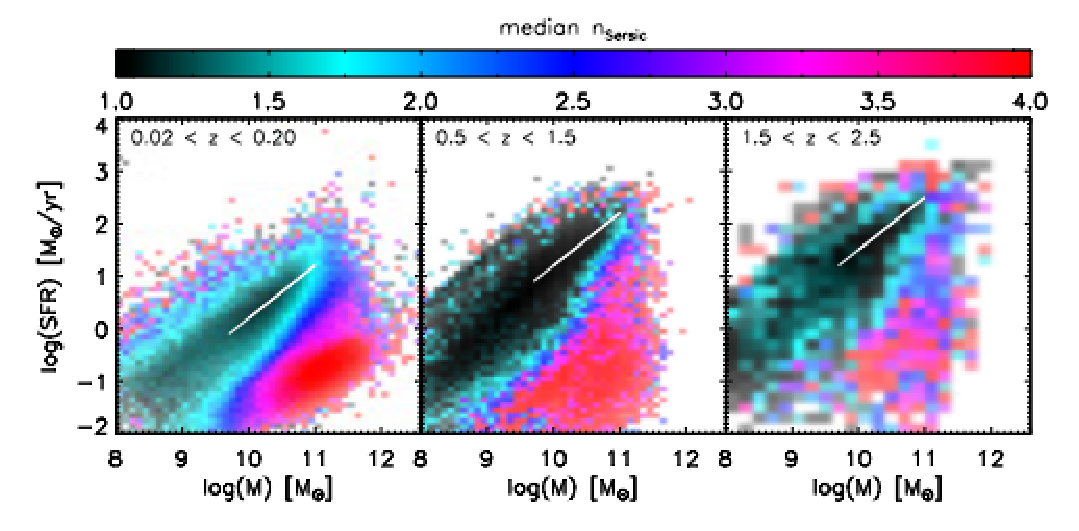
\includegraphics[width=120mm]{\thisdir figs/wuyts1.eps}
}
\caption{
Sersic index, $n$, is presented depending on the location on the
 SFR--M$_{*}$ diagram \citep{wuyts11}. 
The star forming galaxies which are deviated from the main sequence 
(solid white line) tend to have slightly higher $n$, indicating more
 light is present at the center due to a nucleated star burst. 
}
\label{fig:}
\end{figure}

\begin{figure}%[htbp]
\centerline{
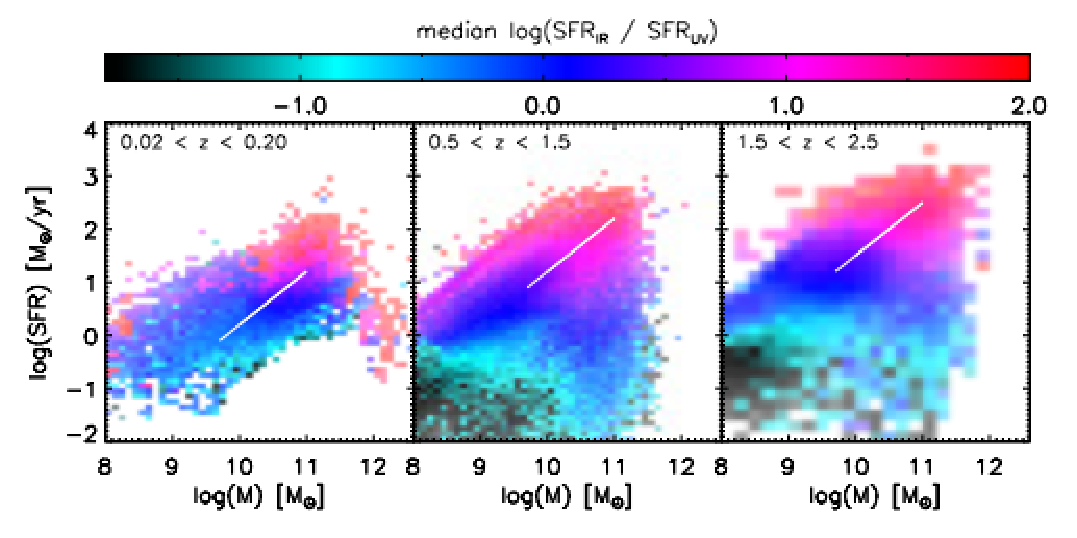
\includegraphics[width=120mm]{\thisdir figs/wuyts2.eps}
}
\caption{
The ratio of SFR measured at infrared and that measured at UV, as an
 indicator of dust extinction is plotted depending on the location of
 the SFR--M$_{*}$ diagram \citep{wuyts11}. 
The star forming galaxies which are deviated from the main sequence 
(solid white line) tend to have higher SFR(IR)/SFR(UV) ratios,
 suggesting the presence of compact dusty star forming regions at the
 center. 
}
\label{fig:}
\end{figure}


\begin{figure}%[htbp]
\centerline{
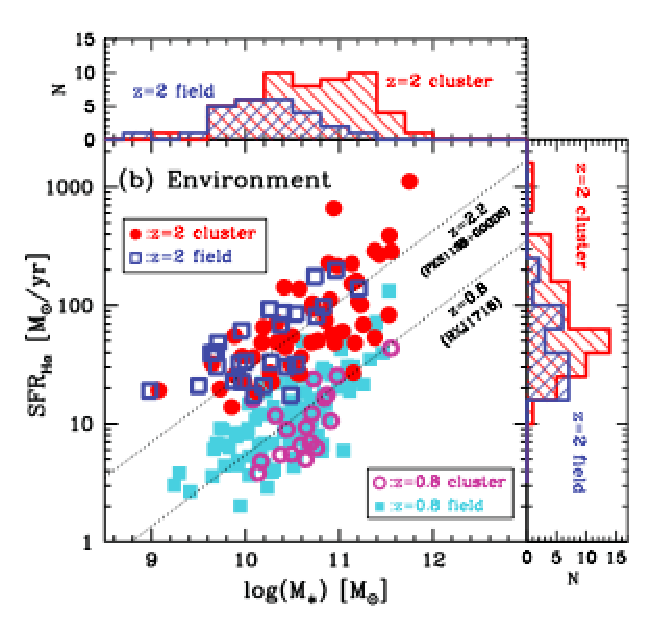
\includegraphics[height=90mm]{\thisdir figs/koyama13.eps}
}
\caption{
Environmental dependence of the ``main sequence'' of star forming
 galaxies at $z\sim2$. 
Red filled circles and blue open squares show galaxies in a
 proto-cluster and those in the general field, respectively 
\citep{koyama13a}.
The location of the main sequence does not depend on
 environemnt. However, the galaxy distribution along the main sequence 
 does depend on the environment in the sense that star forming galaxies
 in the proto-cluster tend to be systematically more massive than 
those in the field.
}
\label{fig:}
\end{figure}

\begin{figure}%[htbp]
\centerline{
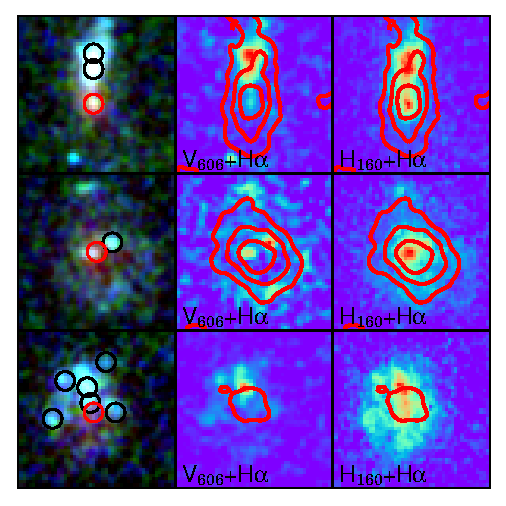
\includegraphics[height=80mm]{\thisdir figs/tadaki14.eps}
}
\caption{
Three H$\alpha$ emitters at $z$=2.16--2.53 with resolved dusty
 star-forming clumps. From left to right, three color images of
 V$_{606}$-I$_{814}$-H$_{160}$, V$_{606}$-band images, and
 H$_{160}$-band images are presented. Contours display the H$\alpha$
 flux density maps derived from NB (MOIRCS) and BB (WFCAM) images whose
 PSF sizes are matched to $\sim$0.7$''$. Red and black circles in right
 panels indicate the positions of the reddest clump nearest to the
 galactic center and other bluer clumps, respectively 
 \citep{tadaki14}.
}
\label{fig:}
\end{figure}


\bibliographystyle{apj}
\bibliography{\thisdir hizpeak}
%%\newpage
%%\bibliography{glao_report}

%\bibitem{madau96} Madau, P., et al., 1996, MNRAS, 283, 1388 
%\bibitem{lilly96} Lilly, S.~J., et al., 1996, ApJ, 460, L1 
%\bibitem{hopkins06} Hopkins, A.~M., \& Beacom, J.~F. 2006, ApJ, 651, 142 
%\bibitem{brinchmann04} Brinchmann, J., et al., 2004, MNRAS, 351, 1151 
%\bibitem{elbaz07} Elbaz, D., et al., 2007, A\&A, 468, 33 
%\bibitem{daddi07} Daddi, E., et al., 2007, ApJ, 670, 156 
%\bibitem{whitaker12} Whitaker K.~E., et al., 2012, ApJ, 754, L29 
%\bibitem{wuyts11} Wuyts S., et al., 2011, ApJ, 738, 106 
%\bibitem{dressler1980} Dressler A., 1980, ApJ, 236, 351 
%\bibitem{lewis2002} Lewis I., et al., 2002, MNRAS, 334, 673 
%\bibitem{gomez2003} G{\'o}mez P.~L., et al., 2003, ApJ, 584, 210 
%\bibitem{peng2010} Peng Y.-j., et al., 2010, ApJ, 721, 193 
%\bibitem{balogh2004} Balogh M., et al., 2004, MNRAS, 348, 1355 
%\bibitem{koyama13a} Kodama, Y., et al., 2013, MNRAS, 428, 1551
%\bibitem{koyama13b} Kodama, Y., et al., 2013, MNRAS, 434, 423

%\bibitem{kodama07} Kodama, T., et al., 2007, MNRAS, 377, 1717
%\bibitem{kodama13} Kodama, T., et al., 2013, IAUS295, in press
%\bibitem{genzel11} Genzel, R., et al., 2011, ApJ, 733, 101
%\bibitem{dekel09} Dekel, A., et al., 2009, Nature, 457, 451
%\bibitem{grogin11} Grogin, N., et al., 2011, ApJS, 197, 35
%\bibitem{tadaki13} Tadaki, K., et al., 2013, ApJ, in press
%\bibitem{tadaki14} Tadaki, K., et al., 2014, ApJ, in press

%\bibitem{vandokkum08} van Dokkum, P.~G., et al., 2008, ApJ, 677, L8
%\bibitem{vandokkum10} van Dokkum, P.~G., et al., 2010, ApJ, 709, 1018
%\bibitem{vandokkum13} van Dokkum, P.~G., et al., 2013, ApJ, 771, L35
%\bibitem{elmegreen05} Elmegreen \& Elmegreen 2005, ApJ, 627, 632
%\bibitem{guo12} Guo, Y., et al.,  2012, ApJ, 757, 120
%\bibitem{genzel06} Genzel, R., et al., 2006, Nature, 442, 786
%\bibitem{tacconi10} Tacconi, L.~J., et al., 2010, Nature, 463, 781
%\bibitem{inoue12} Inoue \& Saitoh 2012, MNRAS, 422, 1902
%\bibitem{barnes} Barnes \& Hernquist 1996, ApJ, 471, 115

%\end{document}

% 20131222
\def\thisdir{science/ga/}
%\documentclass[12pt,letter,times]{cv}
%\usepackage[T1]{fontenc}
%\usepackage{arev}
%\usepackage{setspace}
%\usepackage{graphicx}
%\usepackage{natbib}
%\usepackage{amssymb}
%\usepackage{float}
%\singlespacing
\newcommand*{\bull}{{\scriptsize $\bullet$\hspace{0.15cm}}}

\section{The Galaxy and nearby galaxies
\label{sec:ga}}

\noindent
%\\vspace{5mm}
%\large
\begin{center}
%% Authors
{\bf Alan Walker McConnachie\footnote{NRC Herzberg Institute of
 Astrophysics, Victoria, BC, Canada
 \noindent(alan.mcconnachie@nrc-cnrc.gc.ca)}, 
Masashi Chiba\footnote{Tohoku University, Sendai 980-8578, Japan}, 
Shogo Nishiyama\footnote{NAOJ, Tokyo, Japan}, 
Kim Venn\footnote{University of Victoria, BC, Canada}}
\end{center}
\vspace{0.5cm}

%\author{Alan Walker McConnachie}

%\begin{document}

%\maketitle

%\vspace{-0.25cm}

This report summarizes some relevant science considerations for the
development of a new near infrared (NIR) instrument capability on the
Subaru telescope. The first section discusses possible science drivers
for resolved stellar population studies of our Galaxy, the nearest
galaxies, and related science. In many respects, these science themes
are the ideal science drivers for a NIR instrument assisted by Ground
Layer Adaptive Optics (GLAO) since the science is fundamentally
wide-field and confusion limited. Thus GLAO serves not just as a way of
increasing sensitivity for fainter sources, but is also crucial for
correctly identifying brighter sources. The second section of this
document presents a more general summary of the overall science context
that this new instrument will operate within, and makes a few general
points for future consideration. 

\subsection{The Galaxy and nearby galaxies: Precision insights into galaxy evolution in the nearby Universe}

The nearest galaxies - including our own Galaxy - provide the most
detailed view available on the formation, structure and evolution of
galaxies spanning a broad range of mass and morphological types. This is
primarily achieved by obtaining precision data on the positions, colors,
compositions and kinematics of the many thousands and millions of
individual resolved stars that are accessible to us through observations
on 4 - 10m class facilities. In the future, TMT and the EELT will push
the volume in which this science is possible out to the Virgo cluster
and beyond, bringing within reach nearly every type of major environment
in which galaxies are found, and increasing by orders of magnitude the
number of galaxies for which we can resolve their individual stellar
constituents. Subaru must aim to play a key role in this transformative
and growing research area. TMT and EELT are able to observe ultra-deep
in relatively narrow fields; the focus of Subaru science, therefore,
should be to {\it complement these facilities by providing a wide field
perspective of the stellar populations of the nearest galaxies.} 

\subsubsection{The Galactic Center}

The Galactic Center is a primary target for NIR capabilities on large
telescopes. Massive extinction means that optical surveys are severely
hampered. Depending on the specific science of interest, the potential
area that requires to be surveyed is giant, and demands wide-field
capabilities. This is true not just for imaging but also for
spectroscopy. For many resolved stellar population goals, spectroscopy
is better done in the optical; as well as coinciding with the peak of
the spectral energy distribution (SED), the absence of many strong sky
lines and the high number of atomic transitions  makes the optical
extremely useful, in the absence of other contributing factors. However,
extinction is sufficiently strong in the Galactic Center that the {\it
only} way to obtain spectra for many of the stars is to go to NIR
wavelengths (the recent success of APOGEE, for example, testifies to
this). 

\begin{figure*}[htb]
  \begin{center}
%    \includegraphics[angle=0, width=8cm]{GC_NB}\vspace{-1cm}
    \caption{Identification of intermediate-age stellar populations in
   the Galactic center through narrow band imaging at NIR
   wavelengths. See Nishiyama \& Schodel 2013 for more details.}
  \end{center}
\end{figure*}

There are many precision studies of the Galactic center planned with
forthcoming facilities, for example TMT, in order to look at the proper
motions of stars orbiting the super-massive black hole. However, in
terms of {\it wide-field} science, there are important questions
relating to the bulge stellar populations, star clusters near the center
of the Galaxy (see also next Section) and the connection of the nuclear
star cluster (NSC) to the Galactic SMBH and bulge. In particular,
stellar population identification in the NIR can be aided greatly by the
use of narrow-band filters, to probe specific features and measure the
shapes of the SED (see Figure 1). Constructing detailed star formation
histories further helps us to better understand how star formation
proceeds in the extreme environment of the Galactic Center. However,
overcoming crowding means that this science generally must be assisted
by adaptive optics, else source confusion quickly limits the depth to
which we are able to probe. 

Finally, even although the bulge of the Galaxy is relatively metal-rich,
galaxy formation models suggest that the bulge may be home to the very
first stars that formed in the Universe (so-called Population III
stars). The first stars are believed to form in the highest density
peaks of the early Universe. At zero redshift, these ``peaks'' are to be
found in the centers of galaxies and galaxy clusters. Identification of
candidate stars requires not just high resolution imaging, but also
spectroscopy, ideally assisted with AO to deal with crowding. While
broad wavelength coverage at $R>5000$ is useful for candidate
identification, high resolution ($R>10000-20000$) is required to confirm
the identification of any primordial stars. 

\subsubsection{Milky Way globular clusters}

\begin{figure*}
  \begin{center}
%    \includegraphics[angle=270, width=12cm]{PMclean}\vspace{-0.5cm}
    \caption{Color-magnitude diagrams (CMDs) of globular cluster
   NGC188. The left panel shows the CMD of all stars within the field of
   view, whereas the right panel shows the CMD after removal of all
   stars with high proper motions (Galactic foreground stars). Note that
   the binary sequence running parallel to the main sequence is now
   observable in the cleaned CMD.} 
  \end{center}
\end{figure*}

Globular clusters are unique testbeds for stellar evolution and stellar
dynamics. Their formation and evolution is undoubtedly linked to the
formation of the Milky Way galaxy itself, albeit in ways that are still
not fully understood. Nearby globular clusters subtend relatively large
angles on the sky, and so wide fields of view are particularly
useful. They are also intrinsically crowded environments, and so well
sampled PSFs are essential. Roughly 160 globular clusters are known, and
the median extinction is around a magnitude. Further, in the central
regions of the Galaxy, we are likely missing some globular clusters;
numerous candidates are currently being identified in surveys such as
with UKIRT/WFCAM, and these require follow-up on larger facilities. Near
IR capabilities, ideally supported with adaptive optics to combat severe
crowding, are very useful to help understand the globular cluster
population of the Milky Way.  

As laboratories for the study of stellar populations, it is important
that analysis of the resolved stars in globular clusters accounts fully
for foreground contamination from intervening Galactic stars. Foreground
cleaning is possible with data with high astrometric accuracy:
comparison of images taken at two different epochs will show foreground
stars at slightly different positions relative to the more distant
globular cluster stars, due to their movement between epochs. Analysis
of the resulting CMD can often show features that were otherwise
difficult to identify, for example the binary sequence parallel to the
main sequence of the cluster (see Figure~2). 

With even higher astrometric precision, it is possible to start
constraining the internal dynamics of clusters through their internal
proper motions. Here the rms residuals when matching one epoch to the
other essentially measures the tangential velocity dispersion of the
cluster. Measuring this quantity as a function of radius is of
particular interest, since it is a matter of debate whether massive
black holes exist in the centers of clusters. If they do, they could
have a measurable effect on the dynamics of the stars at these radii,
potentially observable in the proper motions. 

\subsubsection{The nearest galaxies}


\begin{figure*}
  \begin{center}
%    \includegraphics[angle=0, width=7cm]{andi.ps}
%    \includegraphics[angle=0, width=7cm]{peg.ps}\vspace{-2cm}
%    \includegraphics[angle=0, width=6cm]{ic3104.ps}\vspace{-1cm}
    \caption{Structural studies of nearby (dwarf) galaxies. Top panels
   show two local group dwarf galaxies (Andromeda I and Pegasus) at
   distances of around 700kpc. The contours in the first panel and the
   grey-scale in the second panel show the distribution of individual
   stars in these galaxies, and act here as a proxy for surface
   brightness to very low light levels (fainter than
   30mags/sq.arcsec). The contours in the top right panel correspond to
   the HI distribution in Pegasus. Bottom panel: image of IC3104, at a
   distance of around 2.3Mpc. Here, contours tracing the diffuse light
   are overlaid on the $g-$band image. Bright foreground stars are also
   visible. A warp is present in this galaxy, even although it is very
   isolated. Star forming regions are visible. Observational studies of
   this galaxy with excellent IQ can help resolve the global stellar
   populations of this galaxy (in a similar way as for Local Group
   galaxies), examine its wide-field structure, and place future pointed
   observational studies in a global context.}
  \end{center}
\end{figure*}

Beyond the Milky Way lie the $\sim 70-80$ galaxies that are members of
the Local Group. Beyond the Local Group, there are roughly 20 or so
free-floating ``isolated'' galaxies, before we reach the next nearest
galaxy groups at around 3Mpc or so. All of these galaxies are within
reach of current ground based facilities that can resolve their
brightest stars in uncrowded regions. For the majority of galaxies
beyond the Local Group, this is generally limited to the far outer
regions of galaxies, since crowding otherwise prevents us from being
able to distinguish sources from one another in areas of high stellar
density. Further, the ability to distinguish stars from faint,
background galaxies prevents pushing these studies to faint stellar
populations (confusion with galaxies becomes dominant 0.5-1mag brighter
than the magnitude limit of the exposure). This type of resolved stellar
population study allows us to probe not only the ages and metallicities
of the stars, but also the spatial variation of these quantities and the
global structural properties of the galaxy. Figure 3 provides a few
examples of dwarf galaxies that are being studied in this way, in
addition to a more distant dwarf that is an idea target for the Subaru
telescope. 

Studies of nearby galaxies that are outside of the Local Group can offer
valuable insights into galaxy evolution by helping distinguish galactic
evolutionary processes that are internally-driven from externally-driven
environmental effects. Specifically, since dwarf galaxies are low mass,
they are very sensitive to various forms of internal feedback, for
example supernova-driven winds that can stop star formation and  
remove gas from the galaxy to inhibit future generations from
forming. However, examining these effects directly for the closest
dwarfs is complicated by the fact that the majority of nearby dwarfs are
satellite galaxies of either the Milky Way and M31. As satellites, dwarf
galaxies are easily perturbed by their massive hosts. This has a
significant effect on their evolution, for example by removing gas due
to ram pressure stripping or perhaps even by inducing star formation
after pericentric passages (for those dwarfs still with gas). Clearly,
these competing externally- and internally-driven effects obscure each
other, such that it is currently extremely difficult to disentangle
environmental effects from ``intrinsic'' processes. For dwarf galaxies
beyond the Local Group, however, that are not part of neighboring
groups, we can be sure (from timing arguments) that these galaxies have
not been significantly influenced by more massive galaxies. Examination
of their properties therefore can help establish what observed features
are due to processes that are intrinsic to the galaxy, and what effects
are primarily due to environment. 

Subaru is ideally placed to meet this science challenge. Most of the
dwarf galaxies have half-light radii that subtend a few arcmins, but
almost all are found to be very extended and the wide field view is
essential for structural and environmental studies. A stable, well
characterized PSF is essential, and the PSF must be well sampled in
order to be able to distinguish between stars and barely resolved
galaxies near the magnitude limit of the surveys. Small PSFs are
essential to successfully combat crowded fields. 

\subsubsection{Nearby galaxies in the era of the ELTs}


\begin{figure*}
  \begin{center}
%    \includegraphics[angle=0, width=7cm]{ngvs.ps}\vspace{-1cm}
    \caption{Structural studies of distant dwarf galaxies at the
   distance of the Virgo cluster, undertaken in excellent seeing
   conditions (IQ$\sim0.6''$) on CFHT as part of the Next Generation
   Virgo Cluster Survey (NGVS; see Ferrarese et al. 2012). While NGVS
   presents a uniform study of galaxies in the Virgo cluster, a
   comparative uniform wide field study of all galaxies between the
   Local Group and the Virgo cluster is completely lacking. These
   galaxies are the targets for next generation resolved stellar
   population studies with the ELTs. It is therefore essential that
   wide-field NIR photometric studies, ideally equipped with AO, are
   conducted in order to fully capitalize upon TMT resolved stellar
   population science.} 
  \end{center}
\end{figure*}

TMT will be able to obtain deep photometry and even spectroscopy of
individual stars at the distance of the Virgo cluster. Its field of view
is reasonably small, however, and it is not optimized to provide much
detailed information on the environment of the galaxies or their faint
outer regions. Consequently, studies of their global structure need to
be obtained elsewhere in order for forthcoming detailed studies of their
stellar content to be placed in the correct scientific context. {\it
Wide field NIR capabilities are essential to motivate and inform TMT
resolved stellar populations science}. 

At the distance of Virgo, 1\,arcsec corresponds to $\sim 80$pc. Thus,
even without GLAO, wide field surveys of galaxies out to the Virgo
cluster allow mapping of their structural and photometric properties
from the scale of tens of pc to many kpc. To do so, large fields of view
are desirable - at least $\sim 10\times10$ arcmins and preferably
larger. A well characterized, stable, uniform and well-sampled PSF is
essential in order to perform precision morphological modeling and
characterization of each galaxy.

As an example of what can be achieved for galaxies at the distance of
Virgo with good IQ, Figure~4 shows radial profiles derived from optical
ground based observations on CFHT (3.6m) in natural seeing, taken as
part of the Next Generation Virgo Cluster Survey (NGVS). Clearly,
observations with even better IQ and a well characterized PSF can probe
these galaxies at even smaller scales. Already, we are able to probe
their structures over orders of magnitude in scale. Multi-band studies
of these galaxies further probe stellar population variations, and set
the stage for science with the TMT, where the diffraction limited
capabilities allows resolved stellar population studies like those
currently underway for Local Group galaxies. 

Clearly, there already exists, through the NGVS, high quality
homogeneous data on the structures and colors of all galaxies in the
Virgo cluster. However, between the Local Group and Virgo cluster exists
a vast numbers of galaxy groups and ``free-floating'' galaxies, all of
which represent the targets for resolved stellar population studies in
the era of the ELTs. Most are lacking wide field data that probes outer
structures and environments, and certainly there is no homogeneous
analysis of the entire sample or significant subsample. Further, as a
NIR telescope, TMT science will benefit most from having complementary
NIR wide field data. Clearly, this is a significant and crucial role
that Subaru, equipped with a wide field NIR camera, is able to fulfill. 

\subsubsection{Science requirements and possible observing programs}


As is clear from the previous discussion, imaging is more important than
spectroscopy for this science, although studies of the Galactic Center
would certainly benefit from large, multiplexed, AO-assisted
spectrographs. For all science discussed herein, the following are
essential science requirements for an imaging capability: 

\begin{itemize}
\item Broad wavelength sensitivity/coverage (i.e., J, H, K minimum;
      I-band sensitivity desirable to give broad color baseline) 
\item Wide field of view. Minimum of $10 \times 10$\,arcmins. Wider
      field ($\sim$degree) highly desirable 
\item Well-sampled (critically sampled) PSF; stable and
      well-characterized PSF essential 
\item High throughput, to detect faint stars and low surface brightness
      features 
\item Standard broad band filters sufficient, but narrow-band filters
      desirable 
\end{itemize}


For the main imaging science, excellent IQ is required. This increases
sensitivity for the detection of faint objects,  overcomes crowding in
dense stellar environments and is better able to distinguish stars from
faint compact galaxies. A lot of this science is (marginally) possible
at around $IQ\sim0.6''$ (e.g., as exemplified by various studies with
Subaru SuprimeCam and CFHT MegaCam). Better IQ leads to rapidly
increasing science returns. GLAO is therefore an excellent option, and
in many respects the science studies described previously are ideal
science drivers for a GLAO-assisted NIR camera i.e., wide field,
confusion-limited, NIR science. However we note that the gains of GLAO
are lost if the PSF is not critically sampled. Since the delivered IQ
varies depending upon the natural seeing conditions, it is imperative
for this science that the PSF remains critically sampled even in the
best (20\%-ile) condition. 

A possible example of an instrument that could satisfy many of these
requirements is a wide-field camera that can operate at variable
plate-scales. For example, 3 different plate-scales of 0.05''/pix,
0.1''/pix, 0.2''/pix could be implemented, where the first two modes are
used when conditions are excellent or good. The decision as to which
mode is used is driven by the trade-off between good sampling of the PSF
versus required field of view (with the smaller plate scales
corresponding to reduced fields of view). The third mode is used when
natural seeing conditions are poor, such that the resulting IQ is
$\gsim 0.5''$, or when the largest field of view is required. Indeed,
such a mode could additionally be used {\it without} GLAO, perhaps
resulting in an even larger field of view.

Finally, it is worth noting that the development of an adaptive
secondary mirror (ASM) on Subaru is crucial for GLAO. However, it would
also provide a powerful foundation for future instrumentation
development (beyond 2020s), since an ASM makes future adaptive-optics
instruments or techniques (e.g., MOAO, high-contrast imaging, etc)
considerably easier to implement. If Subaru plans to continue NIR
instrumentation development for the long-term, then development of an
ASM would be a powerful investment for future instrumentation to
exploit. 

\subsection{Developing Subaru NIR instrumentation in context}

\subsubsection{Near-IR astronomy in the 2020s, Competition and synergies}

Construction of the Thirty Meter Telescope (TMT) will soon begin on
Mauna Kea. In the south, construction of the European Extremely Large
Telescope (E-ELT) moves ever closer. As correctly identified by Subaru
astronomers, it is essential that the investment in these facilities is
capitalized by ensuring the instruments and facilities exist to ``feed''
these giant telescopes and conduct complementary
observations. Developing a coherent and sustainable plan for telescope
operations in the era of the ELTs should be a major international
priority to ensure the best science can be conducted. Of course, this is
something that will require cooperation between international partners,
and this was nicely reflected in the attendance of the recent meeting on
GLAO science in Sapporo by both Japanese and Canadian astronomers. 

An obvious role for Subaru in the era of TMT is to provide the
wide-field NIR observations that complement the narrow field
observations of TMT. However, it is important to note a few other key
missions and instruments that could also impact the development of a new
NIR instrument on Subaru. 

\par\noindent
{\bf Space-based observatories}

Two major NIR space facilities will be launched towards the end of this
decade. The first, {\bf the James Webb Space Telescope (JWST)}, is a
general-purpose facility and is equipped with both imagers and
spectrographs. It will be unrivaled in its ability to peer into the deep
NIR universe, and obtain excellent spectra up to a resolution of
$R\sim3000$. The second, {\bf Euclid}, will be launched around 2020. It
will undertake a wide field imaging survey of the sky, surveying
15000-20000 square degrees and missing out only the region around the
Galactic plane. It will survey to a depth of Y=J=H=24 at S/N=5 for point
sources. It will have an encircled energy $EA50<0.3''$, and will use
$0.3''$/pixels (although it plans to dither in order to improve spatial
resolution). While the primary purpose of the survey is Dark Energy, the
wide-field NIR legacy imaging dataset that it will produce will be of
immense scientific interest. 

We note that there are other wide field NIR space observatories being
developed, in particular {\bf WISH} and {\bf WFIRST}. Both these
missions are at an earlier stage of development than JWST and Euclid. A
potentially interesting synergy exists with {\bf the Space Infrared
Telescope for Cosmology and Astrophysics (SPICA)}. Here, NIR observation
with Subaru would support the IR and far-IR observations of this
observatory, and could provide a powerful complement that could be
investigated further.  

For NIR observations, space will always be the preferred option, due to
the reduced sky and atmospheric seeing effects. However, it is important
to have complementary observations on the ground. In this respect, it is
vital that any new NIR imaging capability on Subaru... 

\begin{enumerate} 
\item ...has K-band sensitivity (to compliment Euclid)
\item ...is designed to concentrate on studies of the very faint
      Universe, magnitude $>24$ (to compliment Euclid)  
\item ...has a very wide field of view (to compliment JWST)
\end{enumerate}

\par\noindent
{\bf Ground-based instruments}

Aside from the TMT and E-ELT, there are several current and future
wide-field NIR instruments that are AO-assisted and that could impact
the design of a new Subaru capability. Most recent, {\bf Gemini/GeMS},
in the South, is a Multi-Conjugate Adaptive Optic (MCAO) system,
sensitive at J,H,K wavelengths and producing images in K with a 0.08''
FWHM over a 86'' field of view. It has recently been successfully
commissioned and appears to be working well. Since it is MCAO, its field
of view is smaller than achievable with GLAO, but with better
IQ. Gemini/GeMS is probably capable of much of the science discussed in
Section 1.2 (Milky Way globular clusters), since its field of view is
still large enough to observe most of the stars in a globular cluster,
although it would require many pointings to map the large scale
environment of these clusters (e.g., looking for tidal debris). 

Also in the southern hemisphere, VLT is currently converting one of its
Unit Telescopes into an Adaptive Optics Facility (AOF). As part of this
system, they are building a GLAO system,{\bf VLT/Graal}, for use with
Hawk-I, a $7.5'\times7.5'$ field of view imager. The performance of this
system is such that it is expected to become 1.5-2 times ``quicker''
than a seeing limited facility. According to the ESO webpages,  GLAO
will provide Hawk-I with a delivered IQ that is better than 0.5'' at
least 80\% of the time.  

While the Hawk-I camera has a smaller field of view than is possible on
Subaru, it can clearly address some of the science discussed in Section
1, particularly if it tiles observations to map a larger field. In this
respect, we note that it could be worthwhile to examine the case for
developing a wide field NIR instrument that is seeing-limited,
particularly if this means that efficiency can be gained elsewhere. For
example, the metric ``etendue'' is often used to quantify the
``efficiency'' of a camera. Etendue is the product of the telescope
effective area ($A_{eff}$) and the field of view of the camera
($\Omega$). GLAO leads to a higher value of $A_{eff}$ (since it is
quicker at detecting objects), but the value of $\Omega$ for a
GLAO-corrected field is usually considerably smaller than is possible
without adaptive optics. Therefore, {\it for science that is not
confusion-limited, it may be overall more efficient to build a
seeing-limited NIR camera with a very large field of view, rather than a
GLAO-assisted camera with a smaller  field of view}. A decision as to
which approach is better could be determined through examination of the
science, and by comparison of the maximum size of the seeing-limited
field of view to the size of the GLAO-corrected field of view. Clearly,
a seeing-limited camera would not greatly benefit the science discussed
in Section 1, since this science is wide field {\it and}
confusion-limited, and is ideal for a GLAO system. 

\subsubsection{Concluding thoughts}

A new wide-field, NIR capability on Subaru is an exciting and powerful
complement to the instrumentation that will be available on TMT, as well
as to numerous other facilities that will soon be available (e.g., JWST,
Euclid, SPICA). A GLAO-assisted imager would be a powerful tool for
wide-field, confusion-limited science studies, for which resolved
stellar populations and nearby galaxies could be very powerful science
drivers. Depending upon the other science that is envisioned, it could
also be very powerful to develop a seeing-limited, very-wide field
imager (assuming that the seeing-limited field of view is much larger
than the GLAO-corrected field of view). The science impact of either
option, while different, would both be powerful, and would be unique on
Mauna Kea. 

\vspace{2cm}
{\bf Acknowledgments:} We thank the organizers of the Subaru GLAO
science workshop in Sapporo for a very enjoyable and interesting
meeting. We thank Harvey Richer for providing several of the ideas
relating to GLAO observations of globular clusters. 

%\end{document}

%%%%%%%%%%%%%%%%%%%%%%%%%%%%%%%%%%%%%%%%%%%%%%%%%%%%%%%%%%%%%%%%%%%%%%%%%%%%
%% Report format:
%%  - in English
%%  - in Tex(LaTex)
%%  - minimum 4 pages (maximum 10 pages?) per category
%%  - structure
%%      Introduction (summary of past researches, key questions)
%%      New windows to be opened with Subaru GLAO
%%      Proposed observations (obs mode, targets, required # of nights)
%%      Requirements for GLAO and instruments
%%$B!!(B    Synergy/Competitions with other facilities and/or on-going/planed projects
%%      (optional)
%%      Figures, Tables(optional)
%%      References
%%      Any pretty pictures for gravure? (optional)
%%%%%%%%%%%%%%%%%%%%%%%%%%%%%%%%%%%%%%%%%%%%%%%%%%%%%%%%%%%%%%%%%%%%%%%%%%%%

\def\thisdir{science/starplanet/}

%\documentclass[]{article}
%\usepackage{graphicx}
%\usepackage{amsmath,amssymb}
%\usepackage{natbib,aas_macros}
%\citestyle{aa}
%\bibliographystyle{apj}


%\oddsidemargin   -0.2cm
%\evensidemargin  -0.2cm
%\topmargin       -0.2cm
%\textwidth        16.5cm
%\textheight       22.0cm
%\parindent        11pt

%\def\gsim{\mathrel{\raise0.35ex\hbox{$\scriptstyle >$}\kern-0.6em % Greater/squiggles
%\lower0.40ex\hbox{{$\scriptstyle \sim$}}}}
%\def\lsim{\mathrel{\raise0.35ex\hbox{$\scriptstyle <$}\kern-0.6em % Less than/squiggles 
%\lower0.40ex\hbox{{$\scriptstyle \sim$}}}}

%\begin{document}

\section{The Origin of the Initial Mass Function\label{sec:IMF}}

\begin{center}
\noindent
{\bf M. Fukagawa, Y. Oasa, N. Narita}
\end{center}
\vspace{0.5cm}

\normalsize
%%      Introduction (summary of past researches, key questions)
\subsection{Introduction}
\subsubsection{The IMF: Universal or not?}
Understanding the origin of the initial mass function (IMF) has long
been an ultimate goal in the field of star formation, and it has a
crucial impact on study of galaxy evolution. Extensive efforts have been
performed to establish the IMF for a wide range of stellar mass and
cluster density, leading to a well-known functional form, so-called
Salpeter's law; $dN/d(\log m) \propto m^{\Gamma}$, $\Gamma = -1.35$
where $m$ is stellar mass \citep{sal55}. The Salpeter-like IMF appears
almost anywhere at least in the mass range of 0.4--10~$M_{\odot}$
although other types of representations have also been proposed
especially for stars less massive than 1~$M_{\odot}$
\citep{mil79,sca86,sca98,kro01}. The fact that the observed IMFs can be
reasonably well fitted by these functional forms yielded the idea of its
{\it universality}. However, the universality suggests that most, if not
all, stars form in the same way, which may sound unrealistic considering
star formation process in clusters with difference physical properties. 
% such as member density, metallicity, and UV radiation field.

In fact, there are compelling evidences of significant {\it variation}
of the IMF among   star-forming regions or within one cluster
\citep{oas06,hil97}. For instance, \cite{har08} found the flatter IMF
($\Gamma = -0.74$) for the massive Galactic young cluster, NGC 3603,
than the Salpeter-like one, confirming the top-heavy IMF in such
massive clusters and starbursts. At the same time, they identified the
different IMF slopes with the distance from the cluster center,
indicating that massive members are concentrated in the inner region
(Fig.~\ref{fig:imf}). It is worth noting that NGC 3603 is located at
7~kpc (with $A_V =$ 4--5) and harboring O- and B-type stars in a volume
of $<$1~pc$^3$, and the use of adaptive optics (AO) with VLT was
effective to study the IMF for a wide range of stellar mass at the
dense, central region of the cluster. 

Then, the question is, which physical/chemical process/property
determines the shape of the IMF. Is it turbulence, gravity, magnetic
field, metallicity, UV radiation, or interplay of those? To address
this, it is required to further develop observations to establish the
IMF in various environments by obtaining statistically meaningful
sample, where AO can play an important role.  

\subsubsection{How planetary-mass objects form?} 

The low-mass end of the IMF is intimately related to formation mechanism
of planetary-mass objects (PMOs) which is one of the most outstanding,
unsolved problems.  
Free-floating planets, gravitationally unbound to  host stars, have been
discovered in star-forming regions (e.g., \citealt{oas99}) as a natural
extension of the investigation of the stellar IMF. They could form in a
similar way to stars by fragmentation of molecular cloud cores, or in
circumstellar disks as bound planets but ejected by dynamical
instability. The bottom of the IMF can indicate the fragmentation
(opacity) limit, and hence it can reflect main building process for
PMOs. However, even in the deepest surveys, the detections were limited
to objects of a few to 5 Jupiter-masses, and the low-mass end has not
been established yet. On the other hand, the commonality of such
isolated PMOs was also recognized by microlensing, and the possible
change in the mass function at around one Jupiter-mass has been
suggested \citep{sum11}.  


There is one notable implication obtained by recent observations in
young clusters; PMOs found in such young regions are probably less
common than determined by microlensing in the field. In the clusters,
the mass spectrum smoothly extends into the planetary-mass regime down
to $\sim$6~M$_{\rm Jupiter}$ and the slope of the spectrum is not rising
\citep{sch12,pen12}. The planets less massive than 6~M$_{\rm Jupiter}$
might have the distinct mass spectrum. Alternatively, planets found in
microlensing might have experienced the different formation process such
as core accretion in circumstellar disks. It is thus definitely
important to go into the lower mass regime in future observations. It is
also useful to keep in mind when probing less massive members that the
mass of a young planet is usually estimated on the basis of the
evolutionary models which basically assume that planets form like
stars. Such models predict brighter objects than the calculations
supposing the formation through core accretion in  disks
(Fig.~\ref{fig:models}).  Higher sensitivity is the key for future
direct observations towards sub-Jupiter mass planets and to
appropriately interpret the bottom of the IMF. 


%%      New windows to be opened with Subaru GLAO
\subsection{New windows to be opened with Subaru GLAO}

Establishing the IMF under various star-forming environments requires
observations of distant clusters, which demands higher angular
resolution to separate each cluster member as well as higher
sensitivity. In massive star-forming regions, higher angular resolution
is also necessary to probe the cluster centers with being less
contaminated by the brightest stars. Surveys of star-forming regions
have been performed without AO so far since the primary requirement is a
wide field to count enough number of stars to construct the
IMF. Observations utilizing multi-conjugate AO has begun only recently,
but the field-of-view (FoV) is not quite large, $<2'$
\citep{pes13,bou09}.  
The combination of the wider field and AO will certainly enable
efficient observations of more clusters and their central regions.  

Observations basically consist of two steps; photometric detections of
candidate cluster members and spectroscopic follow-ups to accurately
estimate their temperature, surface gravity, and extinction, hence their
memberships and masses. Subaru/MOIRCS is already a powerful tool but it
is problematic that spectra are often overlapped with those of the
neighboring objects. Obtaining ``uncontaminated spectra'' is practically 
important for this science case, and GLAO can contribute to it.  

High sensitivity is important for detection and characterization of
PMOs. In addition, high observing efficiency provided by a large field
is essential to investigate the bottom of the IMF. The very deep
($\sim$2 hours on source), wide-field imaging with GLAO will provide the
detection limit $\sim$3~magnitudes better than the existing surveys of
young clusters. This improvement corresponds to pushing down the lowest
detectable mass from a few Jupiter-masses  to $\lsim$1~M$_{\rm Jupiter}$
for a cluster at 400~pc with $A_V < 1 $ and an age of $\sim$3~Myr, i.e.,
entering sub-Jupiter-mass regime.  On the other hand, observing distant
regions will improve the statistics of the lower-mass IMF, and for
instance, the limiting magnitudes of $J=25$ will enable detections of
massive, embedded PMOs at an age of 1~Myr in NGC 7538 ($d \sim 2.7$~kpc;
$A_V>15$). 


%%      Proposed observations (obs mode, targets, required # of nights)
\subsection{Proposed observations}

The study of the IMF will benefit from very deep, wide-field imaging and
MOS follow-up observations with GLAO. Approximately 30 star-forming
regions within 4~kpc can be potential targets. The required nights
depend on the cluster size, distance, and probably brightness contrast
between the brightest and faintest members. Nevertheless, crudely
assuming no mosaicking (given the planned FoV of $13.'6$ ) and on-source
integration of 2 hours, total $\sim$10 nights are required for the whole
cluster sample for the imaging. Spectroscopic follow-up may need one
night per cluster, and in this case, $\sim$40 nights are necessary. Note
that this is a very crude estimate ignoring the property of each
cluster. For instance, some nearby young clusters and associations are
sparse but good targets for finding less massive PMOs. More nights will
be required for such targets.  

%%      Requirements for GLAO and instruments
\subsection{Requirements for GLAO and instruments}
A wide-field NIR imager and multi-object spectrograph (MOS) is required
for this science case. Photometric estimate of the masses for the
detected sources is not impossible but  includes uncertainties, thus the
spectroscopic capability is needed to confirm the cluster memberships
and to obtain the better determination of their masses. If an integral
field spectrograph is available, disks/jet structures can also be
targeted. The wider FoV is better, but the FoV of $10'$--$14'$, which is
currently planned, would be good enough
(Fig~\ref{fig:spatial_dist}). This may be difficult to achieve, but
higher angular resolution, about $0.''1$ ($< 0.''2$), is quite valuable
to discriminate PMOs from background galaxies based on the morphology.  

It is worth noting that a wide-field NIR imager and MOS is very useful
for exoplanet science although GLAO itself is not critical due to its
relatively low strehl ratio. One of the significant progress in the
field of exoplant has been brought by the Kepler mission, and over 2500
planet candidates were discovered so far, including habitable planets,
Earth-sized or even smaller planets, and circumbinary ones
\citep{bor13,bor11}. However, Kepler's targets are relatively faint and
far, which makes radial-velocity follow-ups for all the candidates
difficult. Further study on atmospheric characterization is also hard to
perform. Thus, as a next step, future planet surveys will target nearby
bright stars to detect and characterize Earth-like or super-Earth
planets especially in the habitable zone, and one such space mission is
TESS (Transiting Exoplanet Surbey Satellite). TESS will employ transit
method for planet detection and currently planned to  be launched in
2017. The important, probably most exciting part of the follow-up of
TESS detections is atmospheric spectroscopy with large-aperture
telescopes. The NIR transmission spectrum is valuable  since NIR is
sensitive to molecules such as CH$_4$, CO, and CO$_2$ while the optical
one is useful to detect Rayleigh scattering \citep{nar13,ben12}
(Fig.~\ref{fig:trans_spec}). In addition, it is observationally a key to
simultaneously obtain spectra for target and reference stars, thus MOS
is the required capability for transmission spectroscopy
\citep{gib13}. It is also preferable to use a narrower slit to reduce
sky background while keeping the slit width to avoid light-loss, but
unfortunately, GLAO cannot contribute much to reduce the slit width due
to the moderate AO correction. Still, it should be emphasized that
wide-field NIR MOS is certainly  useful for characterizing exoplanetary
atmospheres and if a FoV of $\sim$10$'$ is achieved, it will become a
very unique capability among the 8-m class telescopes. 

\vspace{10mm}

\begin{figure}[htbp]
\centerline{
\includegraphics[height=50mm]{\thisdir fig1.eps}
}
\caption{IMFs for NGC 3603 obtained near ($left$) and far from ($right$)
 the cluster center with VLT \citep{har08}. The power-law index of the
 slope is $-0.74$ for the whole cluster, but the steepening with cluster
 radius was observed, indicating mass segregation in the inner
 region. The cluster center was observed with adaptive optics,
 successfully revealing the subsolar mass members in the core of this
 dense cluster. Diamonds and circles indicate the raw and the
 incompleteness corrected mass distributions, respectively. The best-fit
 power-law slopes are shown as a dotted and a dashed line.  The vertical
 dashed and dotted lines indicate the 50\% completeness limit within $r
 \sim 30''$ ($left$) and the detection limit in the outer field
 ($right$). }
\label{fig:imf}
\end{figure}

\begin{figure}
\centerline{
\includegraphics[height=45mm]{\thisdir fig2a.eps}
\hspace{10mm}
\includegraphics[height=45mm]{\thisdir fig2b.eps}
}
\caption{Models of cloudy atmospheres for a planet of 1--10~M$_{\rm
 Jupiter}$ at 400~pc \citep{spi12}. The solid lines correspond to the
 stellar-like formation (cloud fragmentation, disk instability) while
 the dotted ones represent the formation via core accretion in a
 circumstellar disk.}
\label{fig:models}
\end{figure}

\begin{figure}
\centerline{
\includegraphics[height=55mm]{\thisdir fig3a.eps}
\hspace{5mm}
\includegraphics[height=55mm]{\thisdir fig3b.eps}
}
\caption{$Left$: Color composite ($J, H, K_S$) image of S106 obtained
 with Subaru/CISCO \citep{oas06}. The FoV is about $5' \times
 5'$. $Right:$ Spatial distribution of sources detected in S106
 \citep{oas06}. The completeness limit lies in $18 < K' < 20.1$. The
 circles show YSO candidates and the crosses denote field stars. For
 instance, a source with $K'=19.3$ and $A_V=10$ at 1~Myr corresponds to
 6~M$_{\rm Jupiter}$ at the distance of S106 (600~pc).}
\label{fig:spatial_dist}
\end{figure}

\begin{figure}
\centerline{
\includegraphics[height=50mm]{\thisdir fig4a.eps}
\hspace{10mm}
\includegraphics[height=50mm]{\thisdir fig4b.eps}
}
\caption{$Left$: An example of a model transmission spectram of a
 super-Earth atmosphere \citep{ben12}. $Right$: Measured planet-to-star
 radius ratios for a transiting super-Earth GJ 1214b, compared with the
 two best-fit theoretical spectra for the water-rich atmosphere
 \citep{nar13}. A wide-field ($10'$) MOS will be a unique capability and
 very useful to investigate exoplanets' atmospheres.}
\label{fig:trans_spec}
\end{figure}

%\newpage
\bibliographystyle{apj}
\bibliography{\thisdir imf}

%\end{document}


%%% AO Simulation
%%%%%%%%%%%%%%%%%%%%%%%%%%%%%%%%%%%%%%%%%%%%%%%%%%%%%%%%%%%%%%%%%%%%%%%%%
% NGAO$B%o!<%/%7%g%C%WJs9p=q(B                                              %
%%%%%%%%%%%%%%%%%%%%%%%%%%%%%%%%%%%%%%%%%%%%%%%%%%%%%%%%%%%%%%%%%%%%%%%%%
%\documentclass[10pt]{jarticle}
%\usepackage{graphicx}

%\oddsidemargin   -0.25cm
%\evensidemargin  -0.25cm
%\topmargin       -0.25cm
%\textwidth        16.5cm
%\textheight       24.0cm
%\parindent        10pt

%%%%% OYA's personal new commands %%%%%
\newcommand %%%% \protect is necessary for captions %%%%%
{\supstar}{\!\!\mbox{\protect\raisebox{1.5ex}{$\star$}}}
\newcommand{\gtrsim}{\ ^{\displaystyle >}_{\displaystyle \sim}\ }
\newcommand{\lesssim}{\ ^{\displaystyle <}_{\displaystyle \sim}\ }
\newcommand{\adeg}{\hbox{$\,^{\circ}$}}
\newcommand{\arcs}{\hbox{$\,^{\prime\prime}$}}
\newcommand{\arcm}{\hbox{$\,^{\prime}$}}

\def\thisdir{simulation/glao/}

%\begin{document}

\chapter{Next-Generation AO Simulation Study
\label{chap:simulation}}

$BK\>O$G$O$9$P$kK>1s6@<!@$Be9-;kLnJd=~8w3X7O$N$?$a$N(B
$B%7%_%e%l!<%7%g%s$K4p$E$/8!F$7k2L$r$^$H$a$k!#(B
$BJd=~8w3XAuCV(B(AO: Adaptive Optics)$B$N;kLn$r9-$2$k$?$a$K$O!"(B
$BBg5$$f$i$.$N(B3$B<!859=B$$r9MN8$9$kI,MW$,$"$j!"$3$N5;=Q$r%H%b%0%i%U%#!<$H8F$V!#(B
$B%H%b%0%i%U%#!<5;=Q$r4QB,L\E*$K1~$8$F<BAu$9$k$3$K$J$k$,!"$=$NJ}<0$K$OJ#?t(B
$B$"$k(B(\ref{sec:various_ao_systems}$B@a;2>H(B)$B!#(B
$B$=$NCf$G(B
$BCOI=AXJd=~8w3X7O(B(GLAO: Ground-Layer Adaptive Optics)$B$H(B
$BB?E7BNJd=~8w3X7O(B(MOAO: Multi-Object Adaptive Optics)
$B$KBP$7$F%7%_%e%l!<%7%g%s$K$h$k8!F$$r9T$C$?!#(B

$B$9$P$kK>1s6@$K<!@$Be9-;kLn(BAO$B$rMQ$$$?@V30@~4QB,AuCV$,(B
$B3hLv$7;O$a$k:"$K$O!"8}7B(B30m$BK>1s6@$b;OF0$9$k$H4|BT$5$l$k!#(B
$B$9$P$kK>1s6@$N>-Mh7W2h$r9M$($k>e$G$O!"(B
$BL\;X$9%5%$%(%s%9$H$=$l$r<B8=$9$k5;=Q$H$$$&N>LL$K$*$$$F(B
30m$BK>1s6@$H$NAjJd@-$"$k$$$O(B30m$BK>1s6@$X$NH/E8$r0U<1$;$6$k$r$($J$$!#(B
GLAO$B$H(BMOAO$B$H$$$&(B2$B$D$N9-;kLn(BAO$B$NJ}<0$b$3$NMM$JGX7J$rF'$^$($F(B
$B%7%_%e%l!<%7%g%s$K$h$k8!F$$r?J$a$k8uJd$H$7$FA*Br$7$?!#(B
%
GLAO$B$O;kLnD>7B(B10$BJ,0J>e$H$$$&(B
$B9-;k(BAO$B$NCf$G$b:GBg$N;kLn$rC#@.$G$-$kJ}<0$G$"$k!#(B
$BJd@5@-G=$O2s@^8B3&$G$O$J$/%7!<%$%s%0$N2~A1$G$"$k$,!"(B
$B$3$N;kLn$r3h$+$9$3$H$G(B30m$BK>1s6@$HAjJdE*$J2J3XE*8&5f@.2L$,4|BT$G$-$k!#(B
$BFC$K%^%&%J!&%1%"$OBg5$$f$i$.A4BN$NCf$GCOI=AX$,@j$a$k3d9g$,Bg$-$$$3$H$,(B
$BCN$i$l$F$*$j(BGLAO$B$KE,$7$?%5%$%H$G$"$k$H8@$($k!#(B
%
MOAO$B$O9-$$;kLn$KOK$C$FF1;~$KJ#?t$NE7BN$r4QB,$9$k$3$H$G4QB,8zN($r(B
$B>e$2$k$3$H$,$G$-$kJ}<0$G$"$k!#3FE7BN$K$O2s@^8B3&$N6u4VJ,2rG=$,4|BT$G$-!"(B
$BLLJ,8w$H$NAj@-$bNI$$!#(B
MOAO$B$N<B8=$K$O?7$7$$5;=Q3+H/$,I,MW$G$"$k!#(B
$B0E$$4QB,E7BN$+$iN%$l$?J}8~$K$"$k==J,L@$k$$J#?t$NGHLL;2>H@1(B($B%,%$%I@1(B)$B$+$i!"(B
$B4QB,E7BNJ}8~$NGHLL$r?dDj$9$k%H%b%0%i%U%#!<5;=Q!"?dDj$5$l$?GHLL$r(B
$BGHLL%;%s%5(B(WFS)$B$,8+$F$$$J$$J}8~$N2DJQ7A6@(B(DM)$B$GJd@5$9$k%*!<%W%s%k!<%W@)8f5;=Q(B
$BEy$,5s$2$i$l$k!#(B
$B$9$P$kK>1s6@$K$*$$$F5;=QE*!"2J3XE*7P83$rC_@Q$7$F$$$/$3$H$G(B
30m$BK>1s6@$N<!4|4QB,AuCV$KH/E8$5$;$k$3$H$,4|BT$5$l$k!#(B

$B$3$3$G$N%7%_%e%l!<%7%g%s$O9-;kLn2=8!F$$N$?$a$G$"$k$N$G!"(B
$B$$$:$l$NJ}<0$KBP$7$F$b;kLn$r$I$3$^$G9-$/3NJ]$G$-$k$+$,(B
$B:G$b=EMW$J3NG'$9$Y$-E@$K$J$k!#(B
%
GLAO$B$N>l9g$OJd@5@-G=$,%7!<%$%s%0$K6a$$$N$G!"2s@^8B3&$r07$&0lHLE*$J(BAO$B$H$O(B
$B>u67$,0[$J$j%7!<%$%s%0$N1F6A$bBg$-$$!#(B
$B$3$N$h$&$JNN0h$G%7%_%e%l!<%7%g%s7k2L$,@5$7$$$+!"(B
$B$^$?%7!<%$%s%0%b%G%k$r$I$&Dj5A$9$k$+$KCm0U$,I,MW$G$"$k!#(B
%
MOAO$B$N>l9g$O!"8DJLE7BN$KBP$9$k9b%9%H%l!<%kHf$,L%NO$G$"$k$N$G(B
$B2s@^8B3&$N@-G=$r0];}$G$-$k;kLn$,$I$NDxEY$+!"$^$?$=$N$?$a$KI,MW$H$J$k(B
tip/tilt$B%,%$%I@1(B($BDc<!%,%$%I@1(B)$B$N?tEy$N>r7o$,CeL\$9$Y$-E@$G$"$k!#(B
%
$B$3$l$i$N9`L\$r%7%_%e%l!<%7%g%s$K$h$C$F3NG'$7$F$=$l$>$l$NJ}<0$N35MW$rGD0.$7$?(B
$B>e$G!"8!=P46EY$d%9%+%$%+%P%l!<%8$J$I$N$5$i$K>\:Y$J8!F$$X$HH/E8$5$;$F$$$/$3$H(B
$B$K$J$k!#(B

Sec.\ref{sec:gal_sim_imaging}$B$H(BSec.\ref{sec:spec_simulation}$B$G$O!"(B
GLAO$B%7%9%F%`$G$N1sJ}6d2O4QB,$,$I$N$h$&$J$b$N$K$J$k$+!"%J%A%e%i%k%7!<%$%s(B
$B%0$G$N4QB,$d2s@^8B3&$,C#@.$5$l$?>l9g$HHf3S$7$F8!F$$9$k!#(B
Sec.\ref{sec:gal_sim_imaging}$B$G$O;#A|4QB,$K$D$$$F!"(B
Sec.\ref{sec:spec_simulation}$B$G$OJ,8w4QB,$K$D$$$F$^$H$a$k!#(B



\clearpage
\begin{center}

\noindent
\Large
%%$BH/I=FbMF$N%?%$%H%k!JEvF|;H$C$?$b$N$HF10l$G$"$kI,MW$O$"$j$^$;$s!K(B
\section{Simulations of Subaru Next-Gen AO System: GLAO
\label{sec:glao_simulation}}
\vspace{0.5cm}

\noindent
\large
%%$BCx<T(B
{\bf Shin Oya$^1$}\\
$^1$ Subaru Telescope, 650 North Aohoku Place, Hilo, HI 96720, USA\\
\vspace{0.5cm}

\noindent
\normalsize
{\bf Abstract}
\end{center}
\vspace{-0.2cm}

\noindent
%abstract goes here...
$B$3$3$G$O9-;kLnJd=~8w3X7O$NCf$G$b(B10$BJ,3Q$rD6$($k:G$b9-$$;kLn$r3NJ]$G$-$k(B
$BCOI=AXJd=~8w3XAuCV(B(GLAO: Ground-Layer AO)$B$N8!F$7k2L$K4X$7$F5-=R$9$k!#(B
$B$3$NJ}<0$O>eAX$NBg5$$f$i$.$rJd@5$7$J$$$?$a!"2s@^8B3&$N@-G=$rF@$k$3$H(B
$B$G$O$J$/9-$$;kLn$K$o$?$C$F%7!<%$%s%0$r2~A1$9$k$3$H$rL\E*$H$7$F$$$k!#(B
GLAO$B$N<B8=J}K!$H$7$F$O2DJQI{6@$rF3F~$9$kJ}8~$G8!F$$r?J$a$F$$$k!#(B
$B2DJQI{6@$O(BGLAO$B0J30$K$b69;kLn$NE7BN$KBP$7$F9b$$%9%H%l!<%k$rC#@.$9$k(B
$B$3$H$,$G$-$k$N$G!"==J,L@$k$$C10l@1$KBP$9$k<+A3%,%$%I@1(B(NGS)$B4QB,!"(B
$B%3!<%s8z2L$rDc8:$9$k$?$a$NJ#?t%l!<%6!<%,%$%I@1(B(LGS)$B%H%b%0%i%U%#4QB,(B
$B$b9g$o$;8!F$$9$k$Y$-$@$H9M$($F$$$k!#(B
$B%7%_%e%l!<%7%g%s!&%3!<%I$O(BTMT$B$N(BNFIRAOS$B$N$?$a$K3+H/$5$l$?(BMAOS$B$r;HMQ$7$?!#(B



%%$BK\J83+;O!J>ON)$F$O<+M3!K(B

%%% 20130311 ommited by Iwata

%%%%%%%%%%%%%%%%%%%%%%%%%%%%%%%%%%%%%%%%%%%%%%%%%%%%%%%%%%%%%%%%%%%%%%%%%
%% NGAO$B%o!<%/%7%g%C%WJs9p=q%F%s%W%l!<%H(B
%%%%%%%%%%%%%%%%%%%%%%%%%%%%%%%%%%%%%%%%
%%
%% [AO$B$HAuCV$N;EMM(B] $B3F<+MW5a$9$k(BAO$B$dAuCV$N;EMM$r%F%s%W%l!<%H$K$"$kI=$K5-F~!#(B
%%
%% [$B;29MJ88%(B] $BI,$:L@5-$9$k$3$H!#?^$N0zMQ85$bL@5-$9$k$3$H!#(B
%%
%% [$BJ,NL(B] $B4pD49V1i(B(20$BJ,0J>e(B)$B$O(B4$B%Z!<%80J>e!"0lHL9V1i(B(15$BJ,(B)$B$O(B2$B%Z!<%80J>e!#(B
%%
%% [$BDy@Z(B] $B869FDy$a@Z$j(B 2012$BG/(B1$B7nKv(B
%%
%%%%%%%%%%%%%%%%%%%%%%%%%%%%%%%%%%%%%%%%%%%%%%%%%%%%%%%%%%%%%%%%%%%%%%%%%

%\documentclass[10pt]{jarticle}
%\usepackage{graphicx}

%\oddsidemargin   -0.25cm
%\evensidemargin  -0.25cm
%\topmargin       -0.25cm
%\textwidth        16.5cm
%\textheight       24.0cm
%\parindent        10pt

%\def\gsim{\mathrel{\raise0.35ex\hbox{$\scriptstyle >$}\kern-0.6em % Greater/squiggles
%\lower0.40ex\hbox{{$\scriptstyle \sim$}}}}
%\def\lsim{\mathrel{\raise0.35ex\hbox{$\scriptstyle <$}\kern-0.6em % Less than/squiggles 
%\lower0.40ex\hbox{{$\scriptstyle \sim$}}}}

%\begin{document}

\def\thisdir{simulation/moao/}

\begin{center}

\noindent
\Large
\section{Simulations of Subaru Next-Gen AO System: MOAO
\label{sec:moao_simulation}}
\vspace{0.5cm}

\noindent
\large
%%$BCx<T!JNc!K(B
{\bf Masayuki Akiyama$^1$}\\
$^1$ Astronomical Institute, Tohoku University, 3-6 Aramaki, Aoba-ku, Sendai, Japan
\vspace{0.5cm}

\noindent
\normalsize
{\bf Abstract}
\end{center}
\vspace{-0.2cm}

\noindent
$B$3$3$G$O$9$P$kK>1s6@$K$*$$$F(B6$B8D$N%l!<%6!<%,%$%I@1$rMQ$$$F(B
$BB?E7BNJd=~8w3X(B(MOAO)$B$r9T$C$?>l9g$KM=A[$5$l$k@-G=$r8!F$$7$?(B
$B7k2L$r$^$H$a$k!#FC$K!"(BMOAO$B$rMQ$$$k$3$H$GCO>eAXJd=~8w3X(B(GLAO)
$B$h$j$b9b$$Jd=~@-G=$r9-$$NN0h$NB?E7BN$K$D$$$F<B8=$9$k$3$H$r(B
$BL\;X$9!#$=$N$?$a(BGLAO$B$h$j$b9b$$Jd=~@-G=$r0];}$7$D$D!"$I$NDxEY(B
$B$^$G%?!<%2%C%HNN0h$r9-$2$i$l$k$N$+$rI>2A$9$k$3$H$K=EE@$r(B
$BCV$/!#(BMOAO$B$N>l9g$K$O;kLn$NCf$rO"B3E*$KJd@5$9$k$3$H$O$;$:!"(B
$BFCDj$N%?!<%2%C%H$NJ}8~$N$_$NJd@5$r9T$C$F$$$k$3$H$KCm0U$,(B
$BI,MW$G$"$k!#$=$N$?$a0J2<$G$O$3$N%?!<%2%C%H$rA*Br$9$kNN0h$N(B
$B$3$H$r%?!<%2%C%HNN0h$H8F$V!#(B6$B8D$N%l!<%6!<%,%$%I@1$rMQ$$$?(B
$B>l9g!"H>7B(B$3^{\prime}$$BDxEY$N%?!<%2%C%HNN0h$K$D$$$F$O(BGLAO
$B$h$j$b9b$$Jd=~@-G=$,4|BT$5$l$k$,!"$=$l$h$j$b%l!<%6!<%,%$%I@1$N(B
$B4V3V$r9-$2$F%?!<%2%C%HNN0h$r9-$2$k$H;kLn$N$[$H$s$I$NNN0h(B
$B$G(BGLAO$B$K6a$$Jd=~@-G=$7$+F@$i$l$:!"(BMOAO$B$N%a%j%C%H$,(B
$B@8$+$;$J$/$J$k$3$H$,$o$+$C$?!#$^$?<+A3%,%$%I@1$N4V3V$,3+$/$K$D$l(B
$B$F(B Tip-Tilt $B$NGHLL8m:9$,5^7c$KBg$-$/$J$k$3$H$b$o$+$C$?!#(B
Tip-Tilt $B%,%$%I@1$KMQ$$$k$3$H$N$G$-$k<+A3%,%$%I@1$NL@$k$5(B
$B$r9M$($k$H6d6KJ}8~$K$*$$$F$OJ#?t$N<+A3%,%$%I@1$r%?!<%2%C%H(B
$BNN0h$KMQ0U=PMh$k3NN($O$+$J$jDc$/!"(BTip-Tilt $B$NGHLL;D:9$,(B
$B@-G=$r%j%_%C%H$9$k!#(B


%%$BK\J83+;O!J>ON)$F$O<+M3!K(B

%%% 20130311 ommitted by Iwata

% galaxy simulation: imaging
% galaxy simulation: spectroscopy

%%% System Design
%\documentclass[10pt]{jarticle}
%\usepackage{graphicx}
%\usepackage{url}

%\oddsidemargin   -0.25cm
%\evensidemargin  -0.25cm
%\topmargin       -0.25cm
%\textwidth        16.5cm
%\textheight       24.0cm
%\parindent        10pt

%\def\gsim{\mathrel{\raise0.35ex\hbox{$\scriptstyle >$}\kern-0.6em % Greater/squiggles
%\lower0.40ex\hbox{{$\scriptstyle \sim$}}}}
%\def\lsim{\mathrel{\raise0.35ex\hbox{$\scriptstyle <$}\kern-0.6em % Less than/squiggles 
%\lower0.40ex\hbox{{$\scriptstyle \sim$}}}}

\def\thisdir{development/design/}

%\begin{document}

\chapter{System Study for Subaru Next-Generation AO
\label{chap:system_design}}

\section{Comparisons of Candidate AO Systems for Subaru Telescope
 Next-Generation AO
\label{sec:various_ao_systems}}

%%% 20130311 ommited by Iwata

\section{Overview of the System}

%%% 20130311 ommited by Iwata.
%%% Need to include overview of NIR instrument(s) as well?

$B8=;~E@$G5DO@$,?J$a$i$l$F$$$k<!@$Be(BAO$B$*$h$S@V30@~AuCV$N(B
$B4pK\;EMM$rI=(B\ref{tab:spec}$B$K<($7$?!#$3$N;EMM$O:#8e$N>\:Y$J(B
$B8!F$$K$h$C$F$OBgI}$KJQ99$5$l$k2DG=@-$,$"$k!#(B
\begin{table}[t]
\begin{center}
\begin{tabular}{|l|l|l|l|l|}
\hline
 Item & Specification \\
 \hline
 $B4QB,GHD90h(B & 0.9--2.5 $\mu$m ($B%5%$%(%s%9(BWS$B$+$i$NMW5a$O(B0.6--5$\mu$m\\
 $B4QB,%b!<%I(B & $B;#A|!"J,8w!JLLJ,8w$r9MN8$9$k!K(B\\
 $B4QB,;kLn(B & $\phi$ 15$BJ,3Q!J(B20$BJ,3QL\I8!K(B\\
 $B>GE@0LCV(B & $B%+%;%0%l%s>GE@(B \\
 \hline
 $B%,%$%I@1(B & 4 LGS$B!"(BNGS$B!J(B2$\sim$4$B8D$+!)!K(B\\
 $B%,%$%I@1$NA*BrHO0O(B & LGS$B$O4QB,;kLn$NC<!"(BNGS$B$O4QB,;kLnFb(B \\
 $BGHLL%;%s%5!<(B & $B%,%$%I@1$K$=$l$>$l(B1$B$D$:$D(B (Guide star oriented)\\
 $BGHLL%;%s%5!<%?%$%W(B & $B%7%c%C%/%O%k%H%^%s7?!J%T%i%_%C%I7?$bMW8!F$!K(B \\ 
 $BGHLL%;%s%5!<AG;R?t(B & 100$BDxEY$+$=$l0J>e(B ($B9b%9%H%l!<%k$J$i(B1000$BAG;RDxEY$b(B) \\
 $BGHLL%;%s%5!<%5%s%W%j%s%0<~GH?t(B & 500Hz$B0J>e!J(BGLAO$B$O(B100Hz$B$G$b2D!K(B \\
 $B2DJQ7A6@(B & $BI{6@$r2DJQ7A6@2=(B \\
 $B2DJQ7A6@AG;R?t(B & 500$\sim$1000$BDxEY(B \\
 $BGHLL@)8f%b!<%I(B & GLAO (LTAO$B!"(BExAO$B$J$I$X$N@ZBXBP1~$,I,MW$+!)(B)\\
 \hline
\end{tabular}
\caption{$B<!@$Be(BAO$B$*$h$SAuCV$N4pK\;EMM0F(B}
\label{tab:spec}
\end{center}
\end{table}

\section{Technical Challenges}

$B>e=R$7$?(BTomography AO$B$K6&DL$9$k5;=QE*$J2]Bj$O!"(B
$B%l!<%6!<5;=Q$*$h$SJ#?t%l!<%6!<%,%$%I@1$N@=:n5;=Q!"(B
$BBg5$$f$i$.$N9b$5J}8~$N(Btomography$B?dDj5;=Q!"(B
$B2DJQI{6@!"@)8f7W;;5!$J$I$,$"$k!#(B
$B$?$@$7!"@$3&$ND,N.$H$7$F(Btomography AO$B$O@9$s$K(B
$B%7%9%F%`8!F$!"5;=Q8!F$$,?J$a$i$l$F$*$j!"(B
$B5;=QE*$J2]Bj$O$+$J$j9nI~$5$l$D$D$"$k$N$,8=>u$G$"$k!#(B

$B=i4|$N%l!<%6!<%,%$%I@1$O?'AG%l!<%6!<$,<gBN$G$"$C$?!#(B
$B$3$l$O%l!<%6!<G^<A$,1UBN$G$"$j!"0BDj@-!"J]<i@-$K(B
$BBg$-$JO+NO$,I,MW$G$"$k!#$^$??'AG$NNt2=$K$h$k=PNODc2<$,(B
$BHr$1$i$l$J$$!#<!$KH>F3BN%l!<%6!<$H%l!<%6!<7k>=$N(B
$B5;=QH/E8$,$"$j!"8GBN%l!<%6!<$,BfF,$7$F$/$k!#(B
$B:#$G$O%J%H%j%&%`AX$rNe5/$9$k$?$a$NOB<~GHH/@8$rMQ$$$?(B
$BA48GBN%l!<%6!<$,5;=QE*$K@.=O$7$F$-$?!#(B
Gemini$B$N(BMCAO$B$G$O=PNO(B50W$B$N%l!<%6!<$r(B5$B$D$KJ,3d$7$F!"(B
5$B8D$N%J%H%j%&%`%l!<%6!<%,%$%I@1$N:n@.$K@.8y$7$F$$$k!#(B
$B0lJ}!"%U%!%$%P!<%l!<%6!<5;=Q$rMQ$$$?%3%s%Q%/%H$+$D(B
$B0BDj$7$?%l!<%6!<$N3+H/$,(BESO$B$rCf?4$K?J$a$i$l!"(B
$B%I%$%D$N(BTOPTICA$B<R$H%+%J%@$N(BMPB$B<R$N6&F1$G(B
$BO"B3GH(B20W$B$N%l!<%6!<$,@=IJ2=$5$l$?!#(B
$B$3$N%l!<%6!<$OB>$N(B8m$B%/%i%9$N<!@$Be(BAO$B$*$h$S(B
ELT$BMQ(BAO$B$N%l!<%6!<%,%$%I@1MQ8w8;8uJd$H$7$FBg$-$J(B
$B4|BT$,4s$;$i$l$F$$$k!#2f!9$b$9$G$K(BMPB$B<R$H(B
$BHkL)J];}7@Ls$rDy7k$7!"5;=Q>pJs$N8r49!"(B
$B4pK\;EMM$N8!F$=`Hw$r?J$a$F$$$k!#(B
$B$^$?!"%l%$%j!<;6Mp$rMxMQ$7$?%l!<%6!<%,%$%I@1$b(B
WHT$B!"(BMMT$B$J$I$GCOF;$K;n83$,B3$1$i$l$F$$$k!#(B
8m$B%/%i%9$N(Bsingle conjugate $B%l!<%6!<%,%$%I@1(BAO$B$,(B
$B0BDj$7$F1?MQ$5$l$F$*$j!"%l!<%6!<%,%$%I@1$K(B
$B4X$9$k4pAC5;=Q!"1?MQ5;=Q$O$*$*$$$K?JJb$7$?!#(B
$B%l!<%6!<%7%9%F%`$K$D$$$FI=(B\ref{tab:Laser}$B$K$^$H$a$?!#(B

\begin{table}[t]
\begin{center}
\begin{tabular}{|l|l|l|l|l|l|l|l|}
\hline
 %$BK>1s6@(B & Subaru & Keck I & Keck II & Gemini N & VLT  & Gemini S & LBT \\
% \hline
%$B%l!<%6!<%,%$%I@1(B & Na$BAX(B & Na$BAX(B & Na$BAX(B & Na$BAX(B. & Na$BAX(B  & Na$BAX(B & $B%l%$%j!<;6Mp(B \\
%$B%l!<%6!<%?%$%W(B & $BOB<~GH(B & $BOB<~GH(B & $B?'AG(B & $BOB<~GH(B. & $B?'AG(B->$B%U%!%$%P!<(B  & $BOB<~GH(B & $BA48GBN%0%j!<%s(B \\
%$B%l!<%6!<G^<A(B & $B8GBN7k>=(B & $B8GBN7k>=(B & $B?'AGM-5!1UBN(B & $B8GBN7k>=(B. & $B?'AGM-5!1UBN(B->$B8w%U%!%$%P!<(B  & $B8GBN7k>=(B & $B8GBN7k>=(B \\
%$B=PNO(B & $\sim$6W & $\sim$40W & $\sim$15W & $\sim$15W & $\sim$10W->$\sim$25W & $\sim$10W / beacon & $\sim$18W / beacon \\
%$B%l!<%6!<H/?67ABV(B & 143MHz & 75MHz & 13kHz or 26kHz & 75MHz & $BO"B3GH(B & 75MHz & 10kHz \\
$B%,%$%I@1%?%$%W(B & \multicolumn{3}{|c|}{$B%J%H%j%&%`AX(BLGS} &  \multicolumn{1}{|c|}{$B%l%$%j!<(BLGS} \\
\hline
$B%l!<%6!<%?%$%W(B & $B?'AG(B & $BA48GBNOB<~GH(B & $B8w%U%!%$%P!<%l!<%6!<(B & $BA48GBN!!(B\\
\hline
$B%l!<%6!<G^<A(B & $B1UBNM-5!MOG^(B & $B8GBN7k>=(B & $B8w%U%!%$%P!<(B& $B8GBN7k>=(B \\
\hline
$BK>1s6@(B & Keck II & Subaru, Keck I & VLT$B!J<!@$Be!K(B & LBT \\
             & VLT & Gemini N\&S &       &  (Na-LGS$B$b7W2hCf(B) \\
\hline
$B=PNO(B & 15W(Keck II) & 6W(Subaru) & 25W(VLT$B<!@$Be(B) & 18W$\times$3 (LBT) \\
    &    &  40W(Keck I) & & \\
    &  10W(VLT) & 15W(GeminiN) & &  \\
    &    &  10W$\times$5 (GeminiS) & & \\
\hline
$BH/?67ABV(B & 26kHz(Keck II) & 143MHz(Subaru) & $BO"B3GH(B(VLT$B<!@$Be(B) & 10kHz(LBT) \\
  & $BO"B3GH(B(VLT) & 75MHz(Keck I) & & \\
  &   & 75MHz(Gemini N\&S) & & \\
\hline
\end{tabular}
\caption{$B%l!<%6!<%,%$%I@1MQ%l!<%6!<%7%9%F%`$NHf3S(B}
\label{tab:Laser}
\end{center}
\end{table}


$B:GBg3QEY$G$b(B10$BJ,3Q$H$$$&69$$HO0O$N8w8;$rMQ$$$F!"(B
$BESCf$K$"$kBg5$$f$i$.$N(B3$B<!85J,I[$r?dDj$9$k(B
tomography$B?dDj5;=Q$O!"0lHL$N(B3$B<!85(Btomography$B$H$O(B
$B$+$J$j0[$J$kMWAG$r4^$s$G$$$k!#$7$+$7!"B?$/$N(B
AO tomography$B%"%k%4%j%:%`$,Ds>'$5$l!"7W;;5!(B
$B%7%_%e%l!<%7%g%s!"%F%9%H%Y%C%I$K$h$k<B83$,(B
$B?J$a$i$l$F$-$?!#>\:Y$J8!F$$*$h$S%7%9%F%`$KFC2=$7$?(B
$B8!F$$O$^$@I,MW$G$"$k$,!"4pACE*$J(BAO tomography$B$N(B
$B8&5f$O==J,$J$5$l$F$-$F$$$k!#$9$P$k<!@$Be(BAO$B8!F$(B
$B%o!<%-%s%0%0%k!<%W$O!":#8e>\:Y8!F$$rB3$1$F$$$/M=Dj$G$"$k!#(B

$BFC$K(BGLAO$B$O2DJQI{6@$,=EMW$J%3%s%]!<%M%s%H$H$J$k!#(B
$BF|K\$G$O$^$@2DJQI{6@$N8!F$$O?J$a$i$l$F$$$J$$$,!"(B
$B%"%j%>%J$N(BMMT$B!"(BLBT$B$G$O$9$G$K2DJQI{6@$,Ek:\$5$l!"(B
$BL@$k$$%,%$%I@1$G$h$$Jd@5@-G=$rC#@.$7$F$$$k!#(B
$B$^$?%A%j$N(BVLT$B$N$?$a$N2DJQI{6@$,@=:nCf$G$"$k!#(B
$B$3$l$i$N2DJQI{6@$r@=:n$7$?$N$O%$%?%j%"$N(BMicrogate$B<R$G$"$k!#(B
$B2f!9%o!<%-%s%0%0%k!<%W$O$9$G$K(BMicrogate$B<R$H%3%s%?%/%H$r$H$j!"(B
$B$9$P$kK>1s6@MQ$N2DJQI{6@$N35G08!F$$N=`Hw$r?J$a$F$$$k!#(B

$BJ#?t$N%,%$%I@1!"J#?t$"$k$$$OB?AG;R$N2DJQ7A6@$r@)8f$9$k$?$a$N(B
$B7W;;5!$KMW5a$5$l$k@-G=$OHs>o$K9b$$!#2f!9%o!<%-%s%0%0%k!<%W$O!"(B
$B$^$@@)8f7W;;5!$N8!F$$r;O$a$F$$$J$$$,!"(BTMT$BMQ$N%U%!!<%9%H%i%$%H(BAO
$B$G$"$k(BNFIRAOS$B$N@)8f7W;;5!8!F$$,==J,;29M$K$J$k$H9M$($F$$$k!#(B

\section{Interfaces with the Subaru Telescope -- 20130311Iwata: to be ommitted?}

$B$9$P$kK>1s6@<!@$Be(BAO$B$NBh0l8uJd$G$"$k(BGLAO$B$K$D$$$F!"(B
$BK>1s6@$H$N%$%s%?!<%U%'!<%9$r9M;!$7$?!#(B
GLAO$B$N:GBg$NFCD'$O!"2DJQI{6@$rMQ$$$F$$$k$3$H$G!"(B
$BH?<MLL$,>/$J$/8zN($,9b$$$3$H$,$"$2$i$l$k!#(B
$B=>$C$F!"4QB,AuCV$O%+%;%0%l%s>GE@$K@_CV$9$k$N$,$h$$!#(B
$B$^$?!"(BGLAO$B$G$O(B10$BJ,3Q$rD6$($k;kLn$,L%NO$H$J$C$F$$$k!#(B
$B8=:_;H$o$l$F$$$k%+%;%0%l%s>GE@$N2D;kMQBg5$J,;6Jd@58w3X7O$O(B
$B$=$3$^$G$N;kLn$r3NJ]$G$-$F$$$J$$!#(BGLAO$B$H6a@V30@~4QB,AuCV$N(B
$BAH$_9g$o$;$N$H$-$OBg5$J,;6Jd@58w3X7O$O<h$j30$9I,MW$,$"$k!#(B

$B%+%;%0%l%s>GE@$N4QB,AuCV$N8!F$$b=EMW$G$"$k!#(B
GLAO$B$N9-;kLn$r@8$+$96a@V30@~;#A|J,8wAuCV$r8!F$$9$k>e$G!"(B
$BK>1s6@$N8w3X<}:9!"AuCV$N%5%$%:!"=ENL!"@_7W@=B$2DG=$J8w3X7O$N@_7W(B
$B$J$I$,=EMW$J%U%!%/%?!<$H$J$k!#(B

$B2DJQI{6@$O$9$P$kK>1s6@$N%H%C%W%f%K%C%H$K@\B3$5$l$k!#(B
$B$9$P$kK>1s6@$O<g>GE@It$K9-;kLn%+%a%i$J$I$r(B
$BEk:\$9$k$?$a!"%H%C%W%f%K%C%H8r495!$N=ENL@)8B$,(B
3t$B$G$"$k!#8=:_@=:nCf$N(BVLT$BMQ2DJQI{6@$NAm=ENL$O(B1500kg
$BDxEY$J$N$G7ZNL2=$NEXNO$OITMW$G$"$k!#(B
$B8=:_;HMQCf$N@V30I{6@$OD>7B$,(B1265mm$B$G$"$j!"(B
VLT$B$N2DJQI{6@D>7B$h$j$b<c43Bg$-$$!#(B
$B%+%;%0%l%s>GE@$N(BF$BCM$NJQ99$b9MN8$7$?2DJQI{6@$N;EMM:vDj$r(B
$B:#8e?J$a$F$$$/$3$H$K$J$k!#(B
$B%H%C%W%f%K%C%H$K$*$1$kEENO6!5k!"@)8f@~!"%M%C%H%o!<%/!"Nd5Q?e(B
$B$J$I$N4pK\E*$J%$%s%U%i!"%H%C%W%f%K%C%H$H$N%$%s%?!<%U%'!<%9!"(B
$B$J$I$N8!F$$b=EMW2]Bj$G$"$k!#(B

\section{Subaru GLAO System Structure}


%%% 20130311 ommitted by Iwata

%%% 20130311 additions by Iwata
\section{Components of GLAO: Adaptive Secondary Mirror}

\section{Components of GLAO: Wavefront Sensing System}

\section{Components of GLAO: Laser System}

\section{Components of GLAO: RTC}

%%% 20130311 additions by Iwata
\section{Telescope Modifications}

\subsection{Top Unit}

\subsection{Cassegrain Focus}

\subsection{Other Areas?}



\section{Operations of GLAO}

$B$9$P$kK>1s6@$O<g>GE@4QB,AuCV$,$"$k$?$a!"2DJQI{6@$r>o@_$9$k$3$H$O(B
$B1?MQ>e$G$-$J$$!#$=$N$?$a!"2DJQI{6@$O%H%C%W%f%K%C%H8r49AuCV$r(B
$BMQ$$$FCeC&$9$kI,MW$,$"$k!#$=$N$?$a$N%$%s%?!<%U%'!<%9;EMM$r(B
$B3NDj$7$J$1$l$P$J$i$J$$!#$^$?2DJQI{6@$NIT;HMQ;~$NJ]4I>l=j$N3NJ]$H(B
$B$=$N%$%s%?!<%U%'!<%9$H%$%s%U%i$N;EMM$K$D$$$F$b7h$a$kI,MW$,$"$k!#(B
$B$^$?!"8r49;~$N4D6->r7o!"?6F0>r7o!"6@$NJ];}$"$k$$$O0BA4$J>uBV4IM}$K(B
$B$D$$$F$b8!F$$rMW$9$k!#(B

$B0lJ}!"$9$P$kK>1s6@$NI{6@$OFLLL$G$"$k!#FLLL$N2DJQI{6@$N%-%c%j%V%l!<%7%g%s(B
$BJ}K!$K$D$$$F$b8!F$$,I,MW$@!#$^$?!"2DJQI{6@$N:F>xCe$NI,MW@-!"Dj4|E*$J(B
$BJ]<i9`L\$J$I$b=i4|8!F$$NCJ3,$G5DO@$7$F$*$/$Y$-$G$"$m$&!#(B

$B%l!<%6!<<M=P%7%9%F%`$O!"K>1s6@$N%;%s%?!<%;%/%7%g%s$K>o@_$9$k$3$H$r(B
$B8!F$Cf$G$"$k!#CeC&$NI,MW@-$O$J$$$,!"%l!<%6!<$NJ]<i!"ItIJ$N8r49!"(B
$B7PG/JQ2=$X$NBP1~!"0BA44IM}$r4^$a$?%l!<%6!<1?MQBN@)$OI,?\$H$J$k!#(B

$BGHLL%;%s%5!<$O%+%;%0%l%s>GE@>eIt$N%+%;%0%l%s%U%i%s%8$H8F$P$l$kCf$K(B
$B@_CV$5$l$k!#$3$NItJ,$O%"%/%;%9$,BgJQFq$7$/!"AuCV$N8N>c!"2~=$$,(B
$BFq$7$$!#$=$N$?$a$N7xO4!"J]<iITMW$NGHLL%;%s%5!<%7%9%F%`8!F$$OBg@Z$G$"$m$&!#(B

\section{Perspective of Future Development}

GLAO$B%7%9%F%`$O<g$H$7$F2DJQI{6@!"%+%;%0%l%s%U%i%s%8$NGHLL%;%s%5!<!"%l!<%6!<(B
$B<M=P7O!"4QB,AuCV$H$$$&9=@.$+$i$J$k!#$3$N%3%s%]!<%M%s%H$OB>$N(BAO$B%7%9%F%`$K(B
$B$H$C$F$b=EMW$J9=@.MWAG$G$"$k!#(B

$B2DJQI{6@$NAG;R?t$O(B1000$BDxEY$H$J$k8+9~$_$G$"$k!#$=$N$?$a!"L@$k$$<+A3%,%$%I@1MQ$N(B
$BGHLL%;%s%5!<$r4QB,AuCVB&$KMQ0U$9$k$H!"%+%;%0%l%s!"%J%9%_%9$N$$$:$l$N>GE@$K$b(B
Extreme AO$BAuCV$,$G$-$k!#$b$A$m$s!"8=B8$"$k$$$O7W2hCf$N9b%3%s%H%i%9%H4QB,AuCV$K$b(B
$B1~MQ$,$G$-$k$G$"$m$&!#2DJQI{6@$OCf4V@V30@~$NAuCV$NGX7J8w$r2!$5$($kMxE@$H$b$J$k!#(B

$B$^$?!"J#?t%l!<%6!<<M=P7O$O(BMOAO$B$KMxMQ$G$-!"2DJQI{6@$O(BMOAO$B$N(Bwoofer$B$H$7$F;HMQ$7!"(B
$B4QB,AuCVB&$K(BMOAO$B$N(Btweeter$B2DJQ7A6@$r$b$?$;$k$3$H$G!"8zN($NNI$$AuCV$,9M0F$G$-$k$G$"$m$&!#(B

$B$3$N$h$&$K(BGLAO$B%7%9%F%`$OK>1s6@5!G=$N%]%F%s%7%c%k$NDl>e$2$r$9$k$b$N$G$"$k!#(B

%\end{document}


%%% Telescope
%%% 20130312 iwata skelton
\def\thisdir{development/telescope/}

\chapter{Interface with Subaru Telescope
\label{chap:tel}}

%%% 20130311 additions by Iwata
\section{Telescope Modifications: Top Unit}

\section{Telescope Modifications: Cassegrain Focus}

\section{Telescope Control Software}

\section{Other Areas?}




%%% Instruments
\def\thisdir{instrument/}

\chapter{Instruments for Subaru Next-Generation AO
\label{chap:inst}}


\section{Requirements on Instrument from Scientific Objectives}

Here we re-summarize the requirements from key science cases on
instrument specifications.

\begin{itemize}
 \item Field of view
 \item Pixel scale
 \item Requirements on broad-band filters (numbers, wavelength coverages)
 \item Requirements on narrow-band filters (numbers, spectral resolution,
      wavelength uniformity, wavelength coverages)
 \item Spectroscopy: Spectral resolution 
 \item Requirements on multi-object spectrograph mode
\end{itemize}

In this chapter we summarize the studies we have made so far on
instruments for ULTIMATE-SUBARU.

\def\thisdir{instrument/optics/}

\begin{center}
\section{Studies of the Optics for the Wide-Field Near-IR Imager and
 Multi-object Spectrograph
\label{sec:inst_optics}}
\vspace{0.5cm}

\noindent
\large
%% authors
{\bf T. Yamamuro$^{1}$, K. Motohara$^{2}$, I. Iwata$^{3}$ and Subaru
Telescope Next-Gen AO Instrument sub-working group}\\
$^1$ Optocraft
$^2$ Institute of Astronomy, University of Tokyo
$^3$ Subaru Telescope, National Astronomical Observatory of Japan
\vspace{0.5cm}

\end{center}

Here we summarize results of studies made by Dr. Yamamuro (Optcraft).
Document Number: CP0046--11--RP001 (w/o FoV split), CP0046--12--RP001 (w
FoV split).

\subsection{Optical Design without FoV Split}

First we studied how wide field of view can be achieved at the
Cassegrain focus of Subaru Telescope with the following conditions:

\begin{itemize}
 \item Single set of optics can be used (i.e., no FoV split is
       considered).
 \item We consider a near-infrared camera and spectrograph. Wavelength
       range is from 0.8$\mu$m to 2.5$\mu$m. The optics will be cooled
       down to about 100K.
 \item The target image quality is to achieve FWHM $<0.15''$ over the
       entire FoV in all of $J$, $H$, $K$-bands.
 \item The focal plane of the instrument should be flat so that we can
       achieve the above image quality by using science detectors with
       flat pixel arrays.
 \item The use of Teledyne H4RG (15$\mu$m pixel size) is assumed.
 \item The sizes of optical components should be feasibile; for example,
       the maximum size of components made of CaF$_2$ and BaF$_2$ should
       be less than 40cm.
\end{itemize}

We examined the two cases on the telescope parameters; (A) the case we
use the existing optical parameters of Subaru Telescope and (B) the case
with new parameters for the secondary mirror and also that the shape of 
primary mirror can be adjusted within the range of the stroke which the
existing mirror actuators are achievable.

Also, we should consider the necessity of field flatner for the
telescope focus. In order to achieve multi-object spectroscopy (MOS), we
need to insert a mask with slitlets at the telescope focus. Since the
Cassegrain focal plane has a curvature, in order to enable the use of
flat MOS mask, we need to insert field flatning lens(es). For the case
A, we show both the case with and without field flatner.

\subsubsection{A. Cases in which Subaru Telescope optical parameters are
   not changed}

Here we show the simplest case where there is no change in the telescope 
parameters and no field flatner is included.
Fig.\ref{fig:optcraft_fig01} is the optical layout. It consists of nine
collimator lenses and seven camera lenses. Lense materials are CaF$_2$, 
BaF$_2$, Fused silica, and ZnSe.The last lens of the camera section is
aspherical. 

\begin{figure}[!ht]
\centerline{
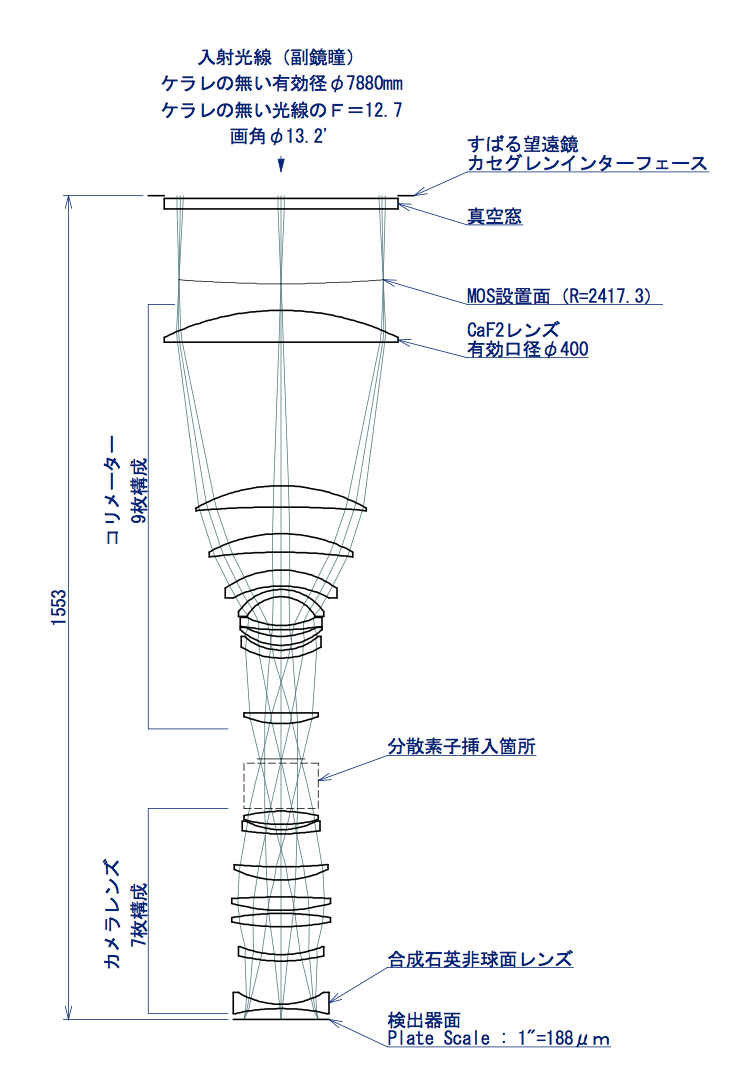
\includegraphics[width=120mm]{\thisdir figs/optcraft_fig01.eps}
}
\caption{Optical layout for Case A: no change in the telescope
 parameters. The case without field flatner.
}
\label{fig:optcraft_fig01}
\end{figure}

The field of view is determined so that the size of effective beam for
the largest lens is within $\phi$400mm, and in this solution it is 
$\phi 13.2'$. The effective diameter of the primary mirror is 
$\phi 7.88$m to achieve the above FoV at the secondary mirror pupil and
to block the light outside of the primary mirror (physical size 
$\phi$8.2m). Since this layout does not include field flatner, the
telescope focal plane has a curvature, and there is astigmatism.

The spot diagram at the position of the MOS mask (with a radius of
curvature of 2417.3mm) is shown in
Fig.~\ref{fig:optcraft_fig02}(left). The degradation of the image toward
the edge of FoV ($\sim 0.2''$ at the edge) is due to astigmatism. 
In this case the slit width at the edge should be adjusted to this image
quality. 
Fig.~\ref{fig:optcraft_fig02}(right) shows the size of distortion at the
position of the MOS mask.

\begin{figure}[!ht]
\centerline{
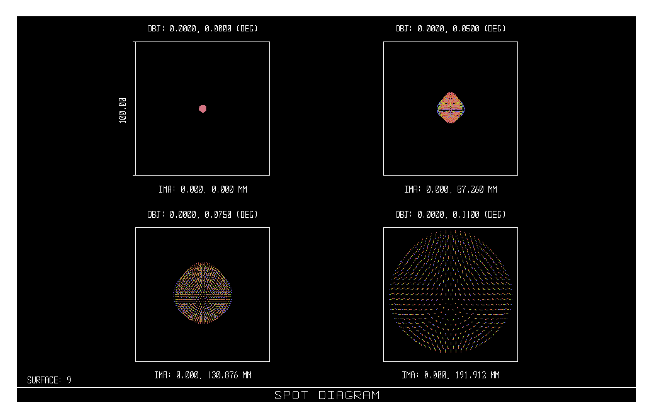
\includegraphics[width=100mm]{\thisdir figs/optcraft_fig02.eps}
 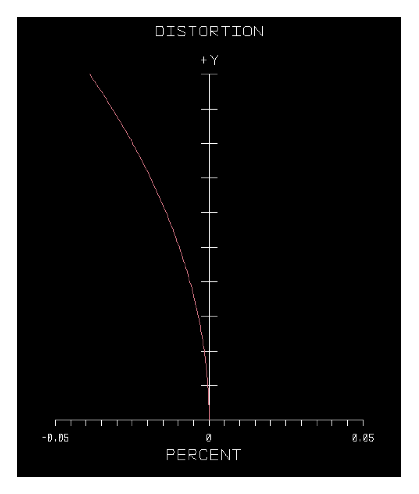
\includegraphics[width=60mm]{\thisdir figs/optcraft_fig03.eps}
}
\caption{(Left) Spot diagram at the position of the MOS mask with a
 curvature radius of 2417.3mm for a configuration shown in 
Fig.\ref{fig:optcraft_fig01}. Spot diagrams with wavelengths from
 0.8$\mu$m to 2.5$\mu$m are shown altogether, as wavelength dependence
 is small. (Right) distortion at the
 position of the MOS mask. The value is $-0.04$\% at the edge.
}
\label{fig:optcraft_fig02}
\end{figure}

The spot diagram and distortion at the position of the detectors are
shown in Fig. \ref{fig:optcraft_fig04}. All FWHM values are smaller than
the target FWHM (0.15$''$) except the case with 0.8$\mu$m
at the edge ($6.6'$) in which the FWHM is slightly larger than
0.15$''$. However, the distortion is large; at the edge it is 
$-6.3$\%.

\begin{figure}[!ht]
\centerline{
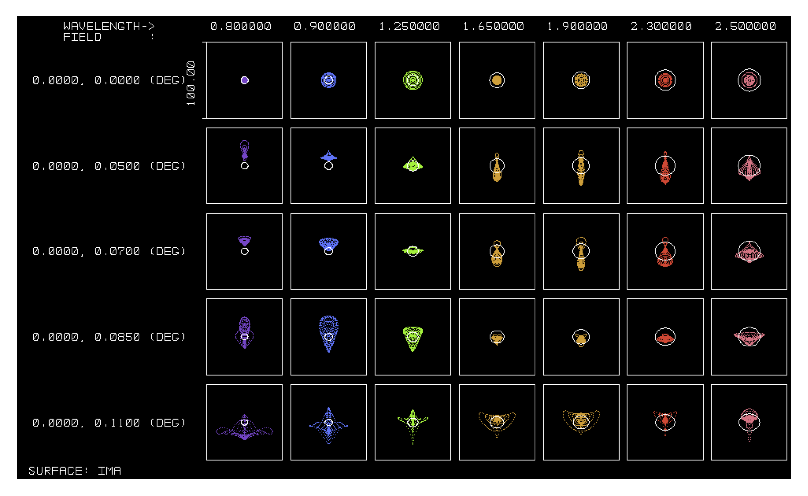
\includegraphics[width=120mm]{\thisdir figs/optcraft_fig04.eps}
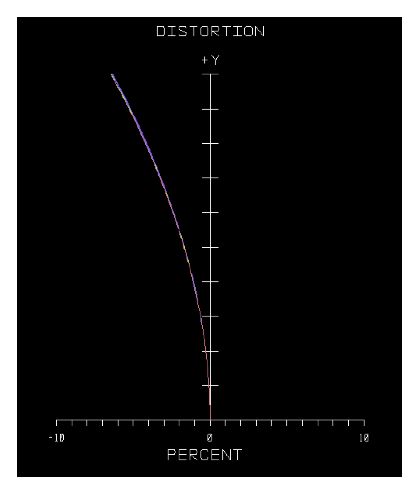
\includegraphics[width=60mm]{\thisdir figs/optcraft_fig05.eps}
}
\caption{(Left) Spot diagram at the position of the detectors for a
 configuration shown in Fig.\ref{fig:optcraft_fig01}.
Five positions from 0$'$ (center) to 6.6$'$ (edge) are shown along the
 vertical axis, and the cases with wavelengths from 0.8$\mu$m to
 2.5$\mu$m are plotted along the horizontal axis. 
The box size is 100$\mu$m which corresponds to 0.53$''$.
(Right) Distortion at the position of the detectors.
}
\label{fig:optcraft_fig04}
\end{figure}


We also evaluated the performance in spectroscopy. As a preliminary
analysis, here we only examined the image quality in spectroscopy in the
range 0.8--2.5$\mu$m without order-sorting.
Fig.~\ref{fig:optcraft_fig06} shows the positions of images in
spectroscopy as a function of wavelength.
Here we assume a fused silica grism with 160 grooves/mm, blaze angle 
34$\circ$\footnote{In section ** we examine more details of various
grisms}.
Fig.~\ref{fig:optcraft_fig07} is the spot diagram. Image qualities at
the shorter and longer wavelength edges and at the edge of FoV is not
good; in 2.5$\mu$m and at $6.6'$ from the center the RMS spot diameter
is $0.22''$. However, it is $0.17''$ at $5.5'$ from the center, and
at the other positions the image quality meets the goal.

\begin{figure}[!ht]
\centerline{
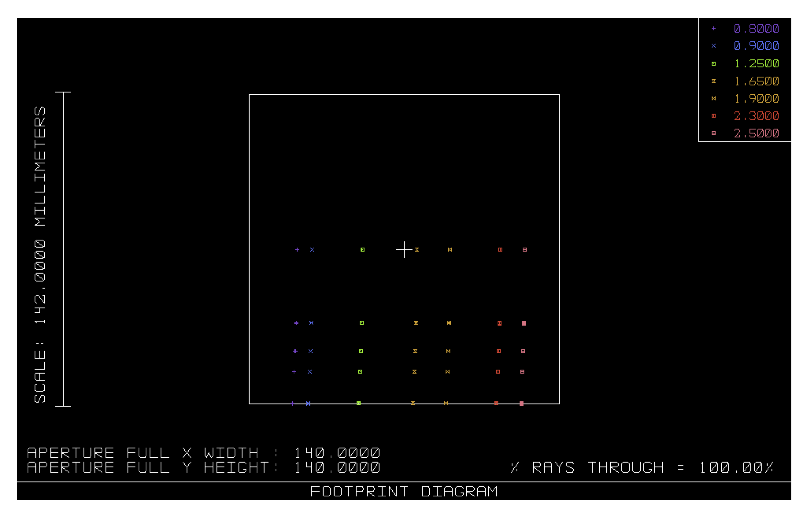
\includegraphics[width=120mm]{\thisdir figs/optcraft_fig06.eps}
}
\caption{Spectroscopic image positions for a configuration shown in Fig.~\ref{fig:optcraft_fig01}.
}
\label{fig:optcraft_fig06}
\end{figure}

\begin{figure}[!ht]
\centerline{
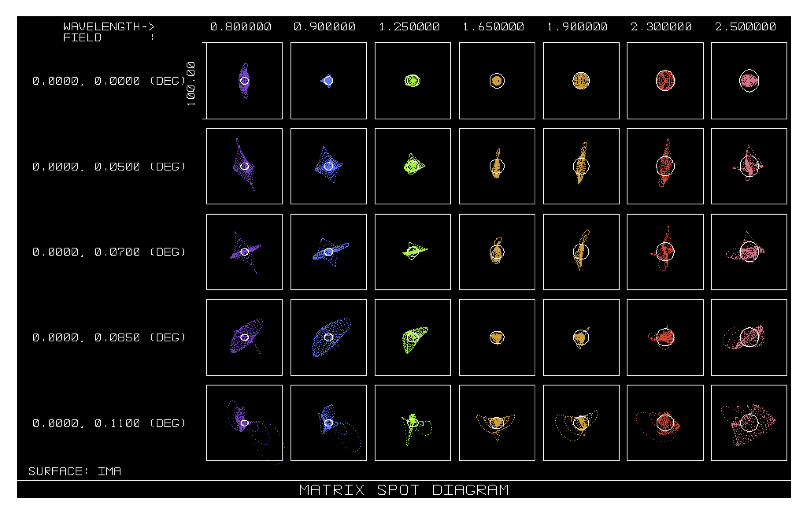
\includegraphics[width=120mm]{\thisdir figs/optcraft_fig07.eps}
}
\caption{Spot diagram for spectroscopy with a configuration shown in
 Fig.~\ref{fig:optcraft_fig01}.}
\label{fig:optcraft_fig07}
\end{figure}

Next we examined the case where there is no change in the telescope
parameters again, and a field flatner which consists of two lenses. 
Fig.~\ref{fig:optcraft_fig08} shows the optical layout of the case.

\begin{figure}[!ht]
\centerline{
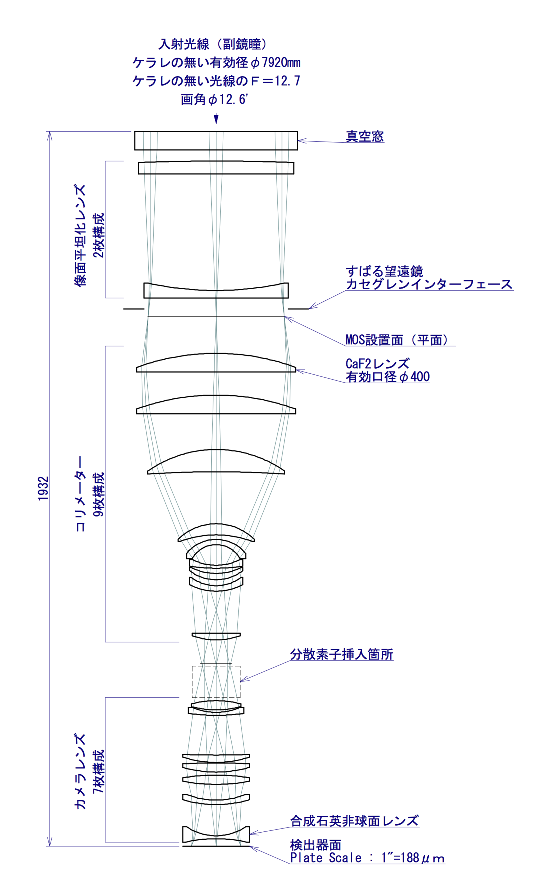
\includegraphics[width=120mm]{\thisdir figs/optcraft_fig08.eps}
}
\caption{Optical layout for Case A: no change in the telescope
 parameters. The case with field flatner.
}
\label{fig:optcraft_fig08}
\end{figure}

The optical design was made so that the effective diameter of the
largest lens is no larger than $\phi$400mm, as it is in the case without
the flatner. The field of view is $\phi 12.6'$, which is slightly
smaller than the case without the flatner, because the field flatner
acts like a concave lens and we need collimator lenses larger than the
flatner. The effective diameter of the primary mirror to block the light
outside of the primary mirror is $\phi$7.92m.
In addition to make the telescope focal plane flat, the addition of the
flatner enables a correction of astigmatism. As shown in 
Fig.~\ref{fig:optcraft_fig09}, the image quality is good at the flat MOS
mask, and there is no chromatic abberation.
We should note that there is distortion, which amounts +0.73\% at the
edge of the FoV.

\begin{figure}[!ht]
\centerline{
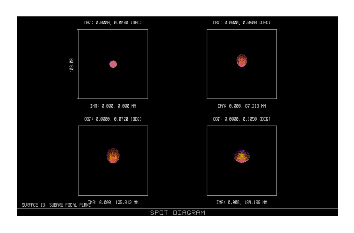
\includegraphics[width=100mm]{\thisdir figs/optcraft_fig09.eps}
 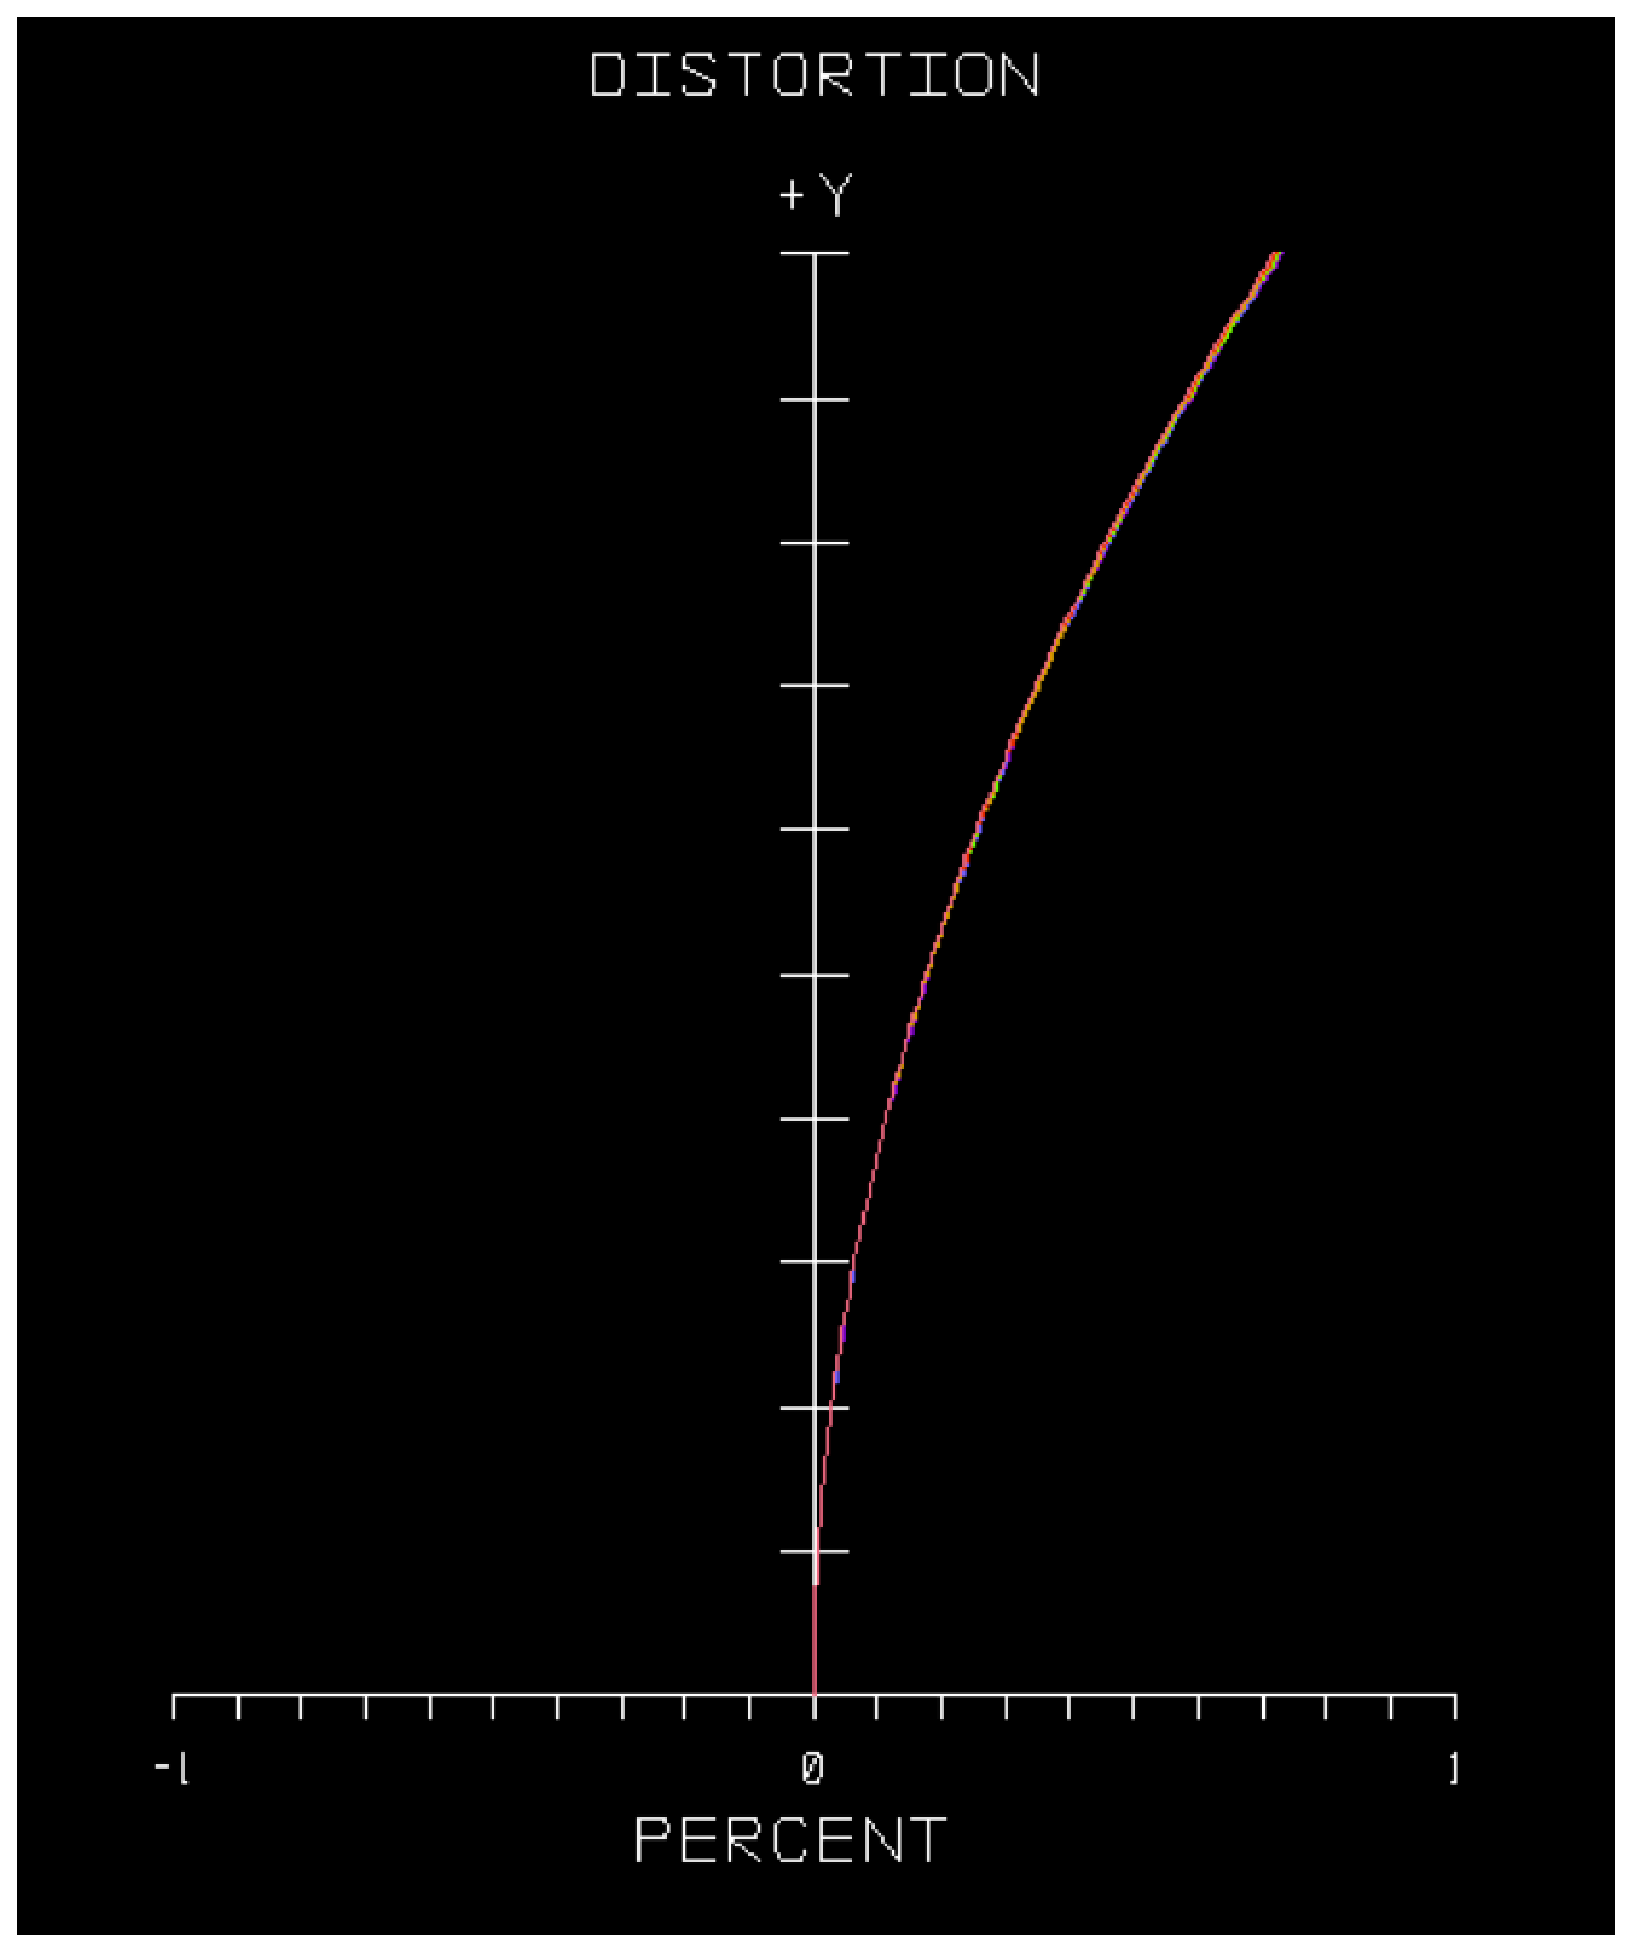
\includegraphics[width=60mm]{\thisdir figs/optcraft_fig10.eps}
}
\caption{(Left) Spot diagram at the MOS mask plate.
(Right) distortion at the MOS mask plate.
}
\label{fig:optcraft_fig09}
\end{figure}

For the image quality at the position of the detectors, similar to the
case without the flatner, in the most of the FoV and for the most of the
wavelength range the image quality satisfies the goal (FWHM smaller than
approx. $0.15''$), while in a few cases (such at the FoV edge ($6.3'$
from the center) and with 0.8$\mu$m) the image quality is slightly worse
than the goal. Distortion is large; it is $-5.2$\% at the edge of FoV.
Performance in the spectroscopy is also similar to the case without the
flatner, and in most cases the qulality satisfies the goal.
We should note that with the field flatner the optical layout is not
telecentric, and the plate scale should be changed if there is a focus
offset.  So the focusing is more important in this case.




\subsubsection{B. Cases in which Subaru Telescope optical parameters are
   changed}

Next we examined the case in which Subaru Telescope's optical parameters
are changed. In order to make the telescope's F number smaller, the
primary mirror's aspheric parameters should be negative. The actuator
storoke for the primary mirror is guaranteed up to 12$\mu$m. We assume
the conic parameters so that displacement at the edge of the primary
mirror is 12$\mu$m, and set F number to be 9.8.

The parameters of the secondary mirror is determined as it is optimal
for this Cassegrain wide-field instrument, and it is independent from
the existing secondary mirrors of Subaru Telescope.
It is a bipolar mirror with a diameter of $\phi$1544mm. The radius of
curvature is 7233.308mm and the conic constant is $-2.35464$.
The field of view is determined by the effective maximum size of the
lens ($\phi$400mm), and it is $\phi16.2'$.
Thanks to the smaller F number, the field of view is 28\% larger than
the case without changing the telescope parameters. The effective
diameter of the primary mirror to avoid the beam outside of the
secondary pupil and primary mirror ($\phi$8.2m) is $\phi$7.93m.

\begin{figure}[!ht]
\centerline{
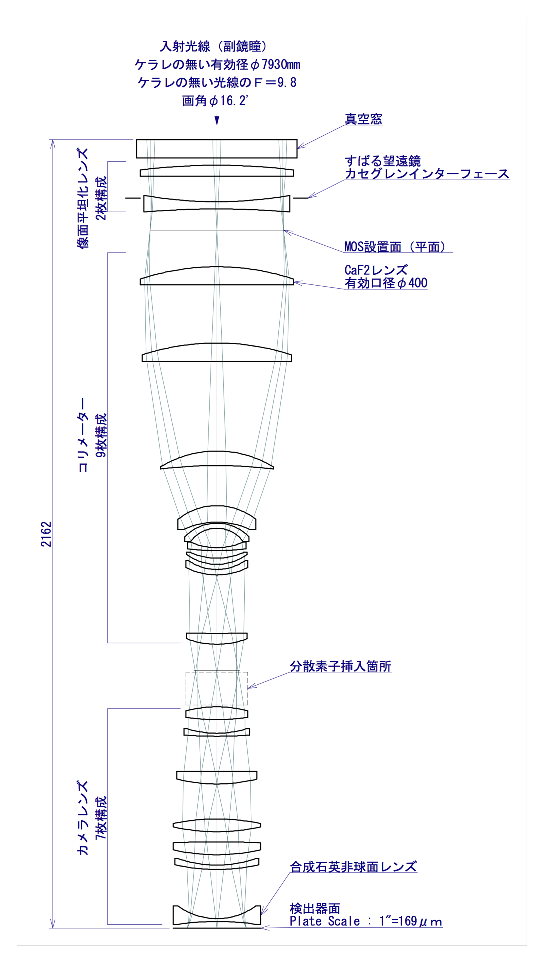
\includegraphics[width=120mm]{\thisdir figs/optcraft_fig15.eps}
}
\caption{The optical layout of the case B: Subaru Telescope
 optical parameters are modified. A field flatner is included in this
 design. 
}
\label{fig:optcraft_fig15}
\end{figure}

In this design a set of lenses as a field flatner is included. 
The spot diagram at the flat MOS mask position is presented in 
Fig. \ref{fig:optcraft_fig16}.
Although small coma aberration is present, its effect is small. There is
no chromatic aberration, overall image quality is good, although there
is distortion aberration at the edge of the FoV.

\begin{figure}[!ht]
\centerline{
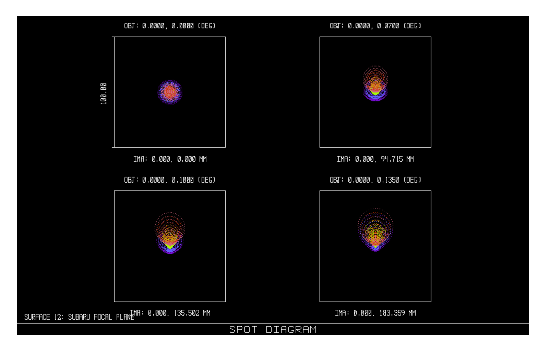
\includegraphics[width=100mm]{\thisdir figs/optcraft_fig16.eps}
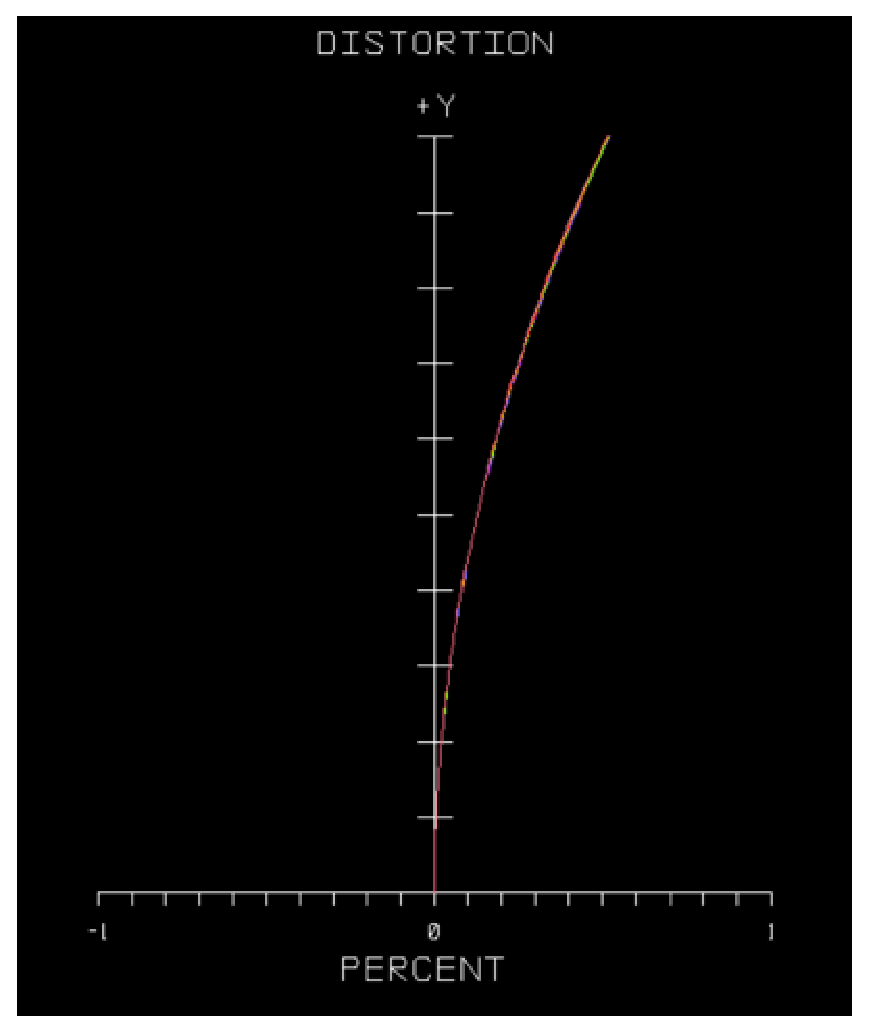
\includegraphics[width=60mm]{\thisdir figs/optcraft_fig17.eps}
}
\caption{(Left) Spot diagram at the MOS mask position.
(Right) distortion aberration at the MOS mask position.
}
\label{fig:optcraft_fig16}
\end{figure}

The configuration of optics after MOS position is similar to the case
without change of the telescope parameters: collimator with nine lenses
and camera with seven lenses. The focal plane is flat. The optical
layout in shown in Fig.\ref{fig:optcraft_fig15}.

In Fig. \ref{fig:optcraft_fig18} we show the spot diagram and distortion
aberration at the position of detectors.
Image quality at outskirt of the FoV ($>6'$) in a short wavelength
(0.8--0.9$\mu$m) degrades by $\sim0.2''$. Otherwise image quality
satisfies the goal (FWHM$\sim 0.15''$).
The maximum distortion aberration at the edge of FoV is $-1.24$\%, which
is smaller than the cases without changes in telescope parameters.

\begin{figure}[!ht]
\centerline{
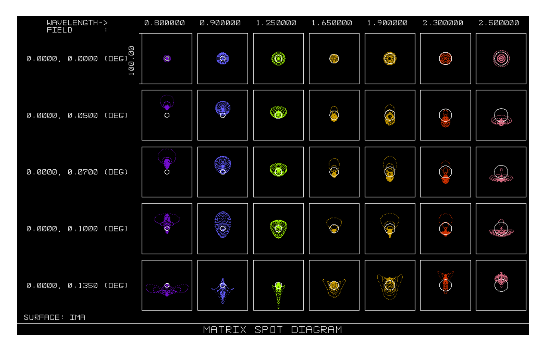
\includegraphics[width=120mm]{\thisdir figs/optcraft_fig18.eps}
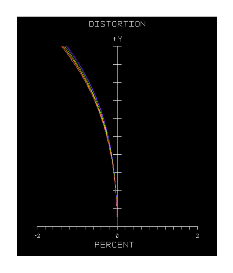
\includegraphics[width=60mm]{\thisdir figs/optcraft_fig19.eps}
}
\caption{(Left) Spot diagram at the positions of the detectors.
Images with five positions within the FoV (vertical) and seven
 wavelengths from 0.8$\mu$m to 2.5$\mu$m (horizontal) are plotted.
The box size is 100$\mu$m, which corresponds to $0.59''$.
The RMS spot diameters are $0.2''$ (at $8.1'$, $0.8\mu$m), 
$0.16''$ (at $6'$, $0.8\mu$m), $0.19''$ (at $6'$, $0.9\mu$m), and for
 other positions and wavelength the spot diameters are within $0.15''$.
(Right) Distortion aberration. It reaches to $-1.24$\% at the edge of
 the FoV.
}
\label{fig:optcraft_fig18}
\end{figure}

Performance in spectroscopy mode is examined and is reported in 
Fig.~\ref{fig:optcraft_fig20}. Here a grism made of fused silica, 160
lines/mm, blaze angle 35$^\circ$ is assumed, and the sizes of spectra on
the detector is presented.

In regards to the image quality, as shown in
Fig.~\ref{fig:optcraft_fig21}, in some cases at the edge of FoV or
shortest/longest wavelengths the RMS spot diameter becomes as large as 
$0.23''$. Otherwise the image quality satisfies the goal, especially
within $6'$ from the center of FoV.

\begin{figure}[!ht]
\centerline{
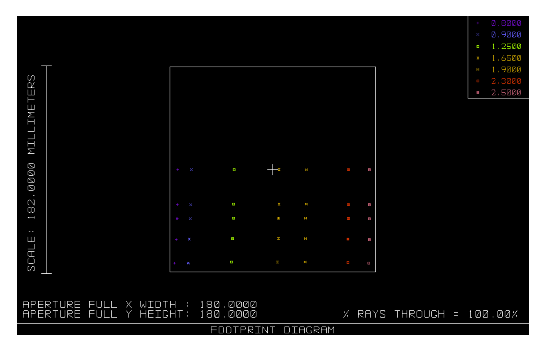
\includegraphics[width=120mm]{\thisdir figs/optcraft_fig20.eps}
}
\caption{
Spectroscopic image positions for a configuration shown in
 Fig.~\ref{fig:optcraft_fig15}. The box size is 180mm. We assume to use
 a grism made of fused silica with 160 lines/mm, and blaze angle
 35$^\circ$.
}
\label{fig:optcraft_fig20}
\end{figure}

\begin{figure}[!ht]
\centerline{
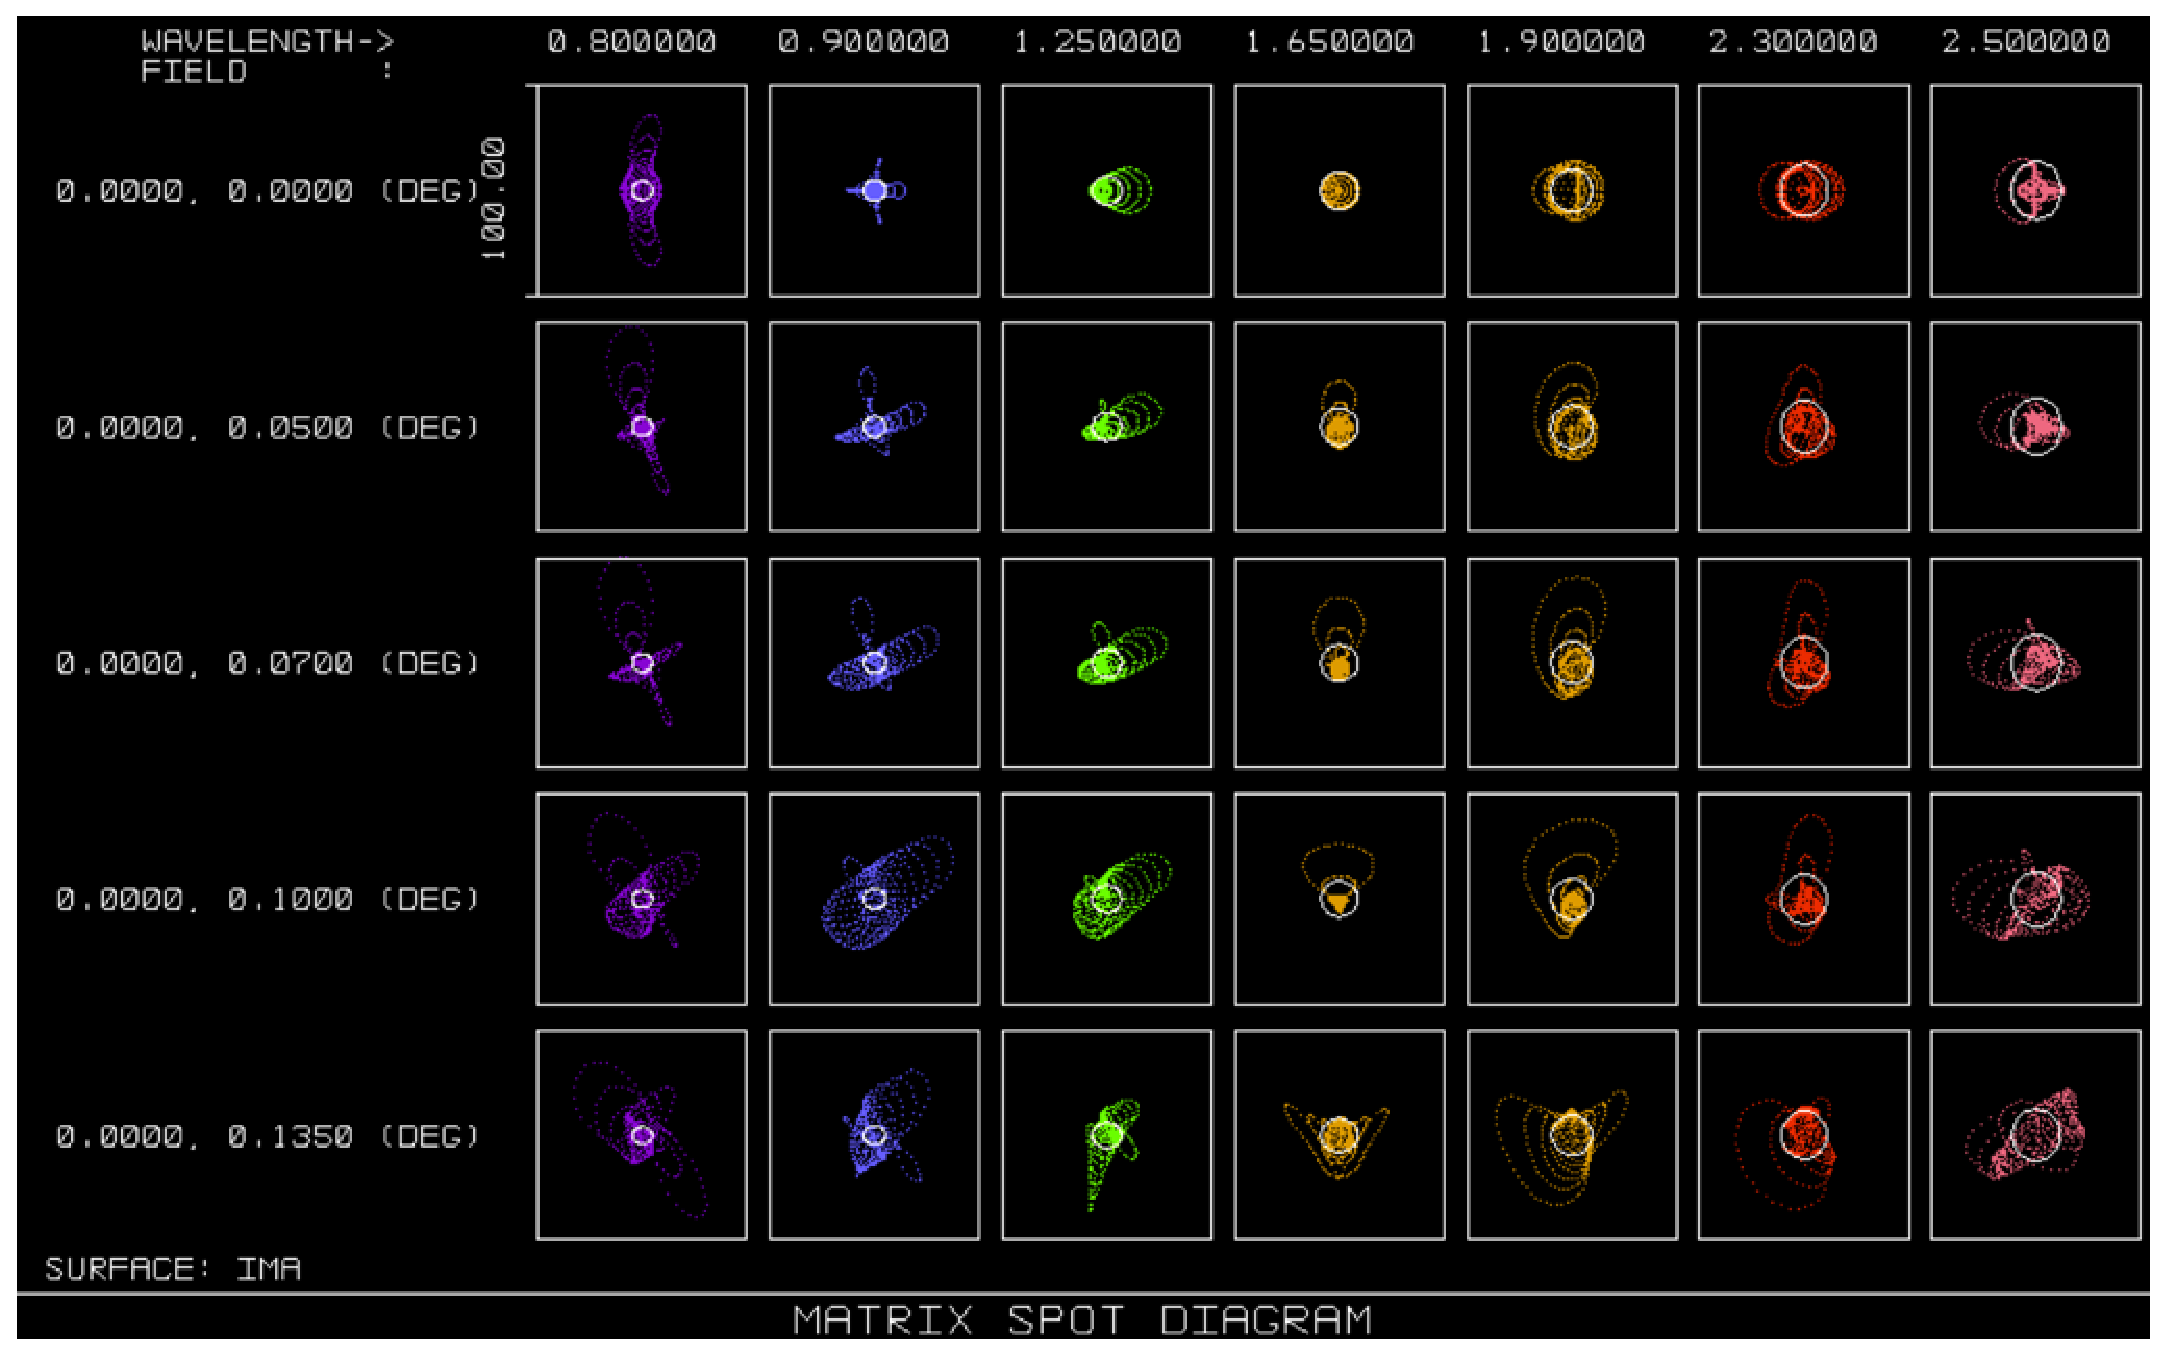
\includegraphics[width=120mm]{\thisdir figs/optcraft_fig21.eps}
}
\caption{Spot diagram for Case B, spectroscopy mode.
In shorter wavelength the performance is somewhat worse than the goal;
 at 0.8$\mu$m RMS spot diameters are in general 0.17--0.18$''$, and 
 0.2$''$ at 0.9$\mu$m. In longer wavelength spot diameter becomes larger
 at positions with distance from the center larger than $6'$ with
 $\lambda = 2.3-2.5\mu$m. Otherwise the image quality satisfies the goal
 ($0.15''$).
}
\label{fig:optcraft_fig21}
\end{figure}



\subsection{Optical Design with FoV Split}

\subsubsection{Case A: secondary mirror parameter is the same as
   existing one}

\subsubsection{Case B: secondary mirror parameter is modified}



\def\thisdir{instrument/mechanics/}

\begin{center}
\section{Studies of the Mechanics for the Wide-Field Near-IR Instrument
\label{sec:inst_mechanics}}
\vspace{0.5cm}

\noindent
\large
%% Authors
{\bf TBD}\\
\vspace{0.5cm}

\end{center}


%%% 20130906 iwata

\section{Optical Design Concept of Wide-field Imager for GLAO}

Proposed by J. Pazder (NRC-NSI-AST / HIA)

\bigskip

\section{Multi Integral-Field-Unit Instrument}

Describe overview of KMOS, discuss feasibility of Multi-IFU instrument
at the Cassegrain focus.

\bigskip

\section{Technical Issues of Wide-field NIR instrument}

\subsection{Mask Exchange Mechanism for MOS}

\subsection{Narrow-band Filters}

\subsection{Size and weight}


%%% Development Plan
\def\thisdir{plan}

\chapter{Development Plan
\label{chap:dev_plan}}

\section{Overview of the Development Plan}

$B$9$P$kK>1s6@$OF|K\$NE7J83X%3%_%e%K%F%#$NK>1s6@$G$"$k!#(B
$B=>$C$F!"$9$P$kK>1s6@<!@$Be(BAO$B$O$=$NE7J83X%3%_%e%K%F%#$N%K!<%:(B
$B$r==J,H?1G$5$;$F@_7W!"@=:n$9$k$Y$-$G$"$k!#(B
$B0lJ}!"$9$P$kK>1s6@$O<+A32J3X8&5f5!9=9qN)E7J8Bf$,1?1D$7$F$$$k!#(B
$B$=$N$?$a!"9qN)E7J8BfA4BN$N>-Mh7W2h$N0lIt$H$7$F$9$P$k<!@$Be(B
AO$B$O?d?J$5$l$J$1$l$P$J$i$J$$!#(B

2012$BG/8=:_!"$9$P$kK>1s6@$G$OD69-;kLn<g>GE@%+%a%i$NN)$A>e$2$,(B
$B?J$a$i$l$F$$$k!#$^$?!"?tJ*2J3X8&5f5!9=$rCf?4$H$7$F!"D69-;kLn(B
$B<g>GE@%U%!%$%P!<J,8w4o7W2h$,;O$a$i$l$?!#0lJ}!"9qN)E7J8Bf$O(B
$BD6Bg7?8w3X@V30@~K>1s6@!"(BTMT$B7W2h$N%Q!<%H%J!<$H$7$F;22h$7$F$$$k!#(B
$B$3$N$h$&$J>u67$NCf$G!"$9$P$kK>1s6@$N<!@$Be@V30@~AuCV$HJ?9T$7$F(B
$B<!@$Be(BAO$B7W2h$,N)$A>e$2$D$D$"$k!#$3$NAuCV7W2h$OF|K\$N8w@V30E7J83X(B
$B%3%_%e%K%F%#$rBeI=$9$k(BSAC$B$N>-MhAuCV9=A[$KDs0F$5$l$F$$$?$b$N$G$"$k!#(B

% comment-out by iwata on 2012/05/07
%$B%7!<%$%s%0%j%_%C%H$N9-;kLnAuCV72(B
%S-CAM,FMOS,MOIRCS (HSC,PFS)
%$B%G!<%?!"%5%$%(%s%9$N7P83$NC_@Q(B
%$B<g>GE@AuCV$r;Y$($k9=B$(B

%$BB>K>1s6@$H$N4X78(B
%8m$B5iK>1s6@$O2?$+$7$i$N9-;kLn(BAO$B7W2h$,$"$k(B
%30m$B5iK>1s6@;~Be$NAjJd@-(B
%    (8m$B$N=88wNO$H3QEYJ,2rG=$@$1$G$O6%AhNO$,$J$/$J$k(B)

$B$9$P$kK>1s6@$N:GBg$NFCD'$O!"<g>GE@D69-;kLnAuCV$G$"$k(BSupreme Cam$B!"(B
FMOS$B!"$=$7$F(B2012$BG/Cf$K%3%_%C%7%g%K%s%0$,3+;O$9$k(BHyper Supreme Cam$B!"(B
$B7W2h$,?J9TCf$N(BPFS$B$G$"$k!#$5$i$K%+%;%0%l%s>GE@$K$O(BFOCAS$B!"(BMOIRCS$B$,(B
$B$"$k!#$3$l$i$N4QB,AuCV$r$D$+$C$?7P83$*$h$S%G!<%?$NC_@Q$O5.=E$G$"$k!#(B
$B$^$?!"$9$P$kK>1s6@$O!"B>$N(B8m$B%/%i%9K>1s6@$H$O0c$$!"<g>GE@AuCV$rEk:\(B
$B$G$-$k$h$&$J7xO4$+$D0BDj$7$?K>1s6@9=B$$r;}$C$F$$$k!#(B2020$BG/Be$K$O!"(B
30m$B%/%i%9K>1s6@$,BfF,$7;O$a$k$?$a!"(B8m$B%/%i%9K>1s6@$N=88wNO$H3QEYJ,2rG=(B
$B$@$1$G$O6%Ah$7$F$$$/$3$H$,$G$-$J$$!#$3$l$i$NE@$r9MN8$7!"(B
$B<!@$Be(BAO$B$*$h$S@V30@~AuCV8!F$%0%k!<%W$O9-;kLn$rBh0l$N%-!<%o!<%I$H$7$F$-$?!#(B
$B$=$N7k2L!"Bh0l8uJd$H$7$F(BGLAO$B$H9-;kLn6a@V30@~;#A|!&(B($BLL(B)$BJ,8wAuCV$r(B
$B<!@$BeAuCV$H$7$F5s$2$?!#(BTMT$B$NsUL@4|!"(BJWST$BEy$N1'ChK>1s6@;~Be$K$*$$$F!"(B
$B$3$NAuCVDs0F$O==J,$J6%AhNO$HO"7HNO$,$"$j!"B>$NCO>e(B8$\sim$10m$B%/%i%9(B
$BK>1s6@$K$*$1$k<!@$BeJd=~8w3X$*$h$S@V30@~AuCV$H$N6%Ah$H=;$_J,$1$,(B
$B2DG=$G$"$k$H4|BT$5$l$k!#(B

$BK\8!F$Js9p=q$NBh(B\ref{chap:science}$B>O$G$O!"9-$$4QE@$+$i$_$?<!@$Be(BAO
$B$*$h$S@V30@~AuCV$K$h$k!":#8eH/E8$9$k$G$"$m$&%5%$%(%s%9%1!<%9$NDs0F$r(B
$B=8$a$?!#<!@$Be(BAO$B$*$h$SAuCV;EMM$KBP$9$kMW5a$N=EMW$J;qNA$G$"$k!#(B
$B0z$-B3$-!"MM!9$J%5%$%(%s%9%1!<%9$K$D$$$F5DO@$r?<$a$F$$$/$Y$-$G$"$k!#(B

$B0lJ}!"(BAO$B$N@-G=%7%_%e%l!<%7%g%s$HL\I8@-G=!"AuCV$N35G08!F$$r?J$a!"(B
$BHs>o$K=iJbE*$JAuCV;EMM$*$h$SAuCV3+H/7W2h$r9M0F$7$D$D$"$k!#(B

$BK\>O$O$=$N7W2h$N35MW$K$D$$$F=R$Y$F$$$/!#(B

\section{Development Organization}

\subsection{International Partnership}


\section{Budget}

\subsection{Fund-Raising Plan}


\section{Development Schedule}



\end{document}


%%%% structure in '2012 Japanese edition of Study Report'

%%% Science
\chapter{Science with ULTIMATE-SUBARU 
\label{chap:science}}

In this chapter we introduce science cases proposed to be carried out
with Subaru Telescope Next-Generation AO (ngAO) and clarify
specifications ngAO and associated new instruments should satisfy.

The GLAO system we are studying have following features (see
Chapter~\ref{chap:system_design} for details):

\begin{itemize}
\item Wide-field seeing improvement by correcting WFE caused by ground
      layer of the Earth's atmosphere. Seeing improvement will provide
      not only better angular resolution, but also the significant
      improvement of sensitivity especially for point-like sources. On
      the other hand, the WFE correction (and subsequently angular
      resolution) for individual sources are not as good as classical AO
      systems (such as AO188 of Subaru) which are designed to achieve
      diffraction-limited image for narrow-field. 
\item Number of optical component should be reduced by using the
      Adaptive Secondary Mirror. This means that thermal emission from
      telescope and instrument should be reduced, and that sensitivity
      at longer wavelength ($\gsim 2\mu$m) will be improved.
\end{itemize}

We have developed studies of the science cases under the recognition of
these features, and with strong interactions with technical studies of
the GLAO system and the associated instruments.

We have two primary scientific objectives (or 'Science Drivers') of this
project. The one is `Complete Sensus of Galaxy Evolution with
Large-Scale Near-IR Surveys', and the other is `Discovery of the Most
Distant Galaxies and Understanding of the Process of the Cosmic
Reionization'.

Because GLAO can provide images with better spatial resolution and
improved sensitivity, the GLAO system can be a `significant upgrade
of Subaru Telescope' rather than an introduction of a new
instrument. Various reseaches should be benefitted with the system.
In Septermber 2011 we had a science workshop in the Japanese community
titled `Science Workshop for Subaru Telescope Next-Gen AO System' in
Osaka,
Japan\footnote{\href{http://www.naoj.org/Projects/newdev/ws11b/index.html}{http://www.naoj.org/Projects/newdev/ws11b/}}. 
We also had 'Subaru GLAO Science Workshop' in June 2013 in Hokkaido
Univ. Some Canadian researchers as well as those from Taiwan has
participated the workshop and presented their prospects. 
Through these workshops, we received important suggestions and proposals
for wide-range of researches, such as galaxy evolution, growth of
massive black holes, galaxy archaeology, the Galactic center,
star-forming regions, and exoplanets. From this science workshop we
started more extensive discussions on various science cases, and this
chapter represents the current outcomes of such discussions and studies.

%\include{science/minowa/minowa}
%\include{science/iwata/ngao_spec_simulation}
\include{science/iwata/legacy_survey}
\def\thisdir{science/veryhighz/}


\section{Search for Galaxies at $z>7$ with Narrow-Band Imaging
\label{sec:nbf}}

\noindent
\begin{center}
%% Authors
{\bf Ikuru Iwata$^{1}$}\\
$^1$ Subaru Telescope, National Astronomical Observatory of Japan, 650
North Aohoku Place, Hilo, HI 96720, USA
\end{center}
\vspace{0.5cm}

\subsection{Introduction}

Subaru has been one of leading facilities pushing the frontier of
the distant universe. A unique capability of the prime focus camera
(Suprime-Cam) have enabled us to conduct wide-field survey which is
essentially important to find very rare objects such as luminous distant
galaxies. One of the efficient methods to find distant star-forming
galaxies is to detect Ly$\alpha$ emission using narrow-band filter (NBF) 
imaging. A strongly star-forming object with a redshift 
$z = \lambda_\mathrm{NBF} / \lambda_\mathrm{Ly\alpha} -1$ could
appear to be bright compared to those with adjacent broad-band
filters. Galaxies detected with this methods are called as 'Ly$\alpha$
emitters (or LAEs)'. The current most distant galaxy with a spectroscopic 
confirmation is an LAE at $z=7.215$, which was discovered by
\citet{Shibuya2012} using Suprime-Cam with a narrow-band filter NB1006
(central $\lambda$ is 10,052\AA).

Currently a new prime focus camera for Subaru Telescope in optical
wavelength, Hyper Suprime-Cam (HSC), is under testing. HSC has more than
seven times wider field-of-view, and it is expected to enable us
conducting deep surveys much more efficiently than the current
Suprime-Cam. HSC will have a NBF called NB101 which has a central
$\lambda$ is 10,095\AA, which will be used to detect many $z\sim 7.3$
LAEs. 
However, the wavelength of the redshifted Ly$\alpha$ is almost at the
long wavelength limit of the CCDs, and finding galaxies at $z>7.5$ with
cameras with CCDs is impossible. So deep near-IR surveys are mandatory
to push the redshift frontier further.

(Cosmic reionization)


\subsection{Surveys with ULTIMATE-SUBARU}

We will use special narrow-band filters which are designed to trace
photons with wavelength ranges between the strong OH air glows from the
Earth's atmosphere.
Here we assume three wavelength ranges as a fiducial set to study the
feasibility.

\begin{table}[!ht]
\begin{center}
\begin{tabular}{rrr}
\hline
$\lambda_\mathrm{c}$ & FWHM & $z_{\mathrm Ly\alpha}$\\
\hline
1.0625 & 0.015  &  7.74\\
1.340  & 0.019  & 10.0 \\
1.550  & 0.022  & 11.75\\
\hline
\end{tabular}
\end{center}
\caption{
Central wavelengths ($\lambda_\mathrm{c}$ in $\mu$m), FWHM (in $\mu$m),
 and redshifts of Ly$\alpha$ emission at $\lambda_\mathrm{c}$ for NBFs
 considered here.
}
\label{tab:iwata_nbf_setup}
\end{table}

\begin{figure}[!ht]
\centerline{
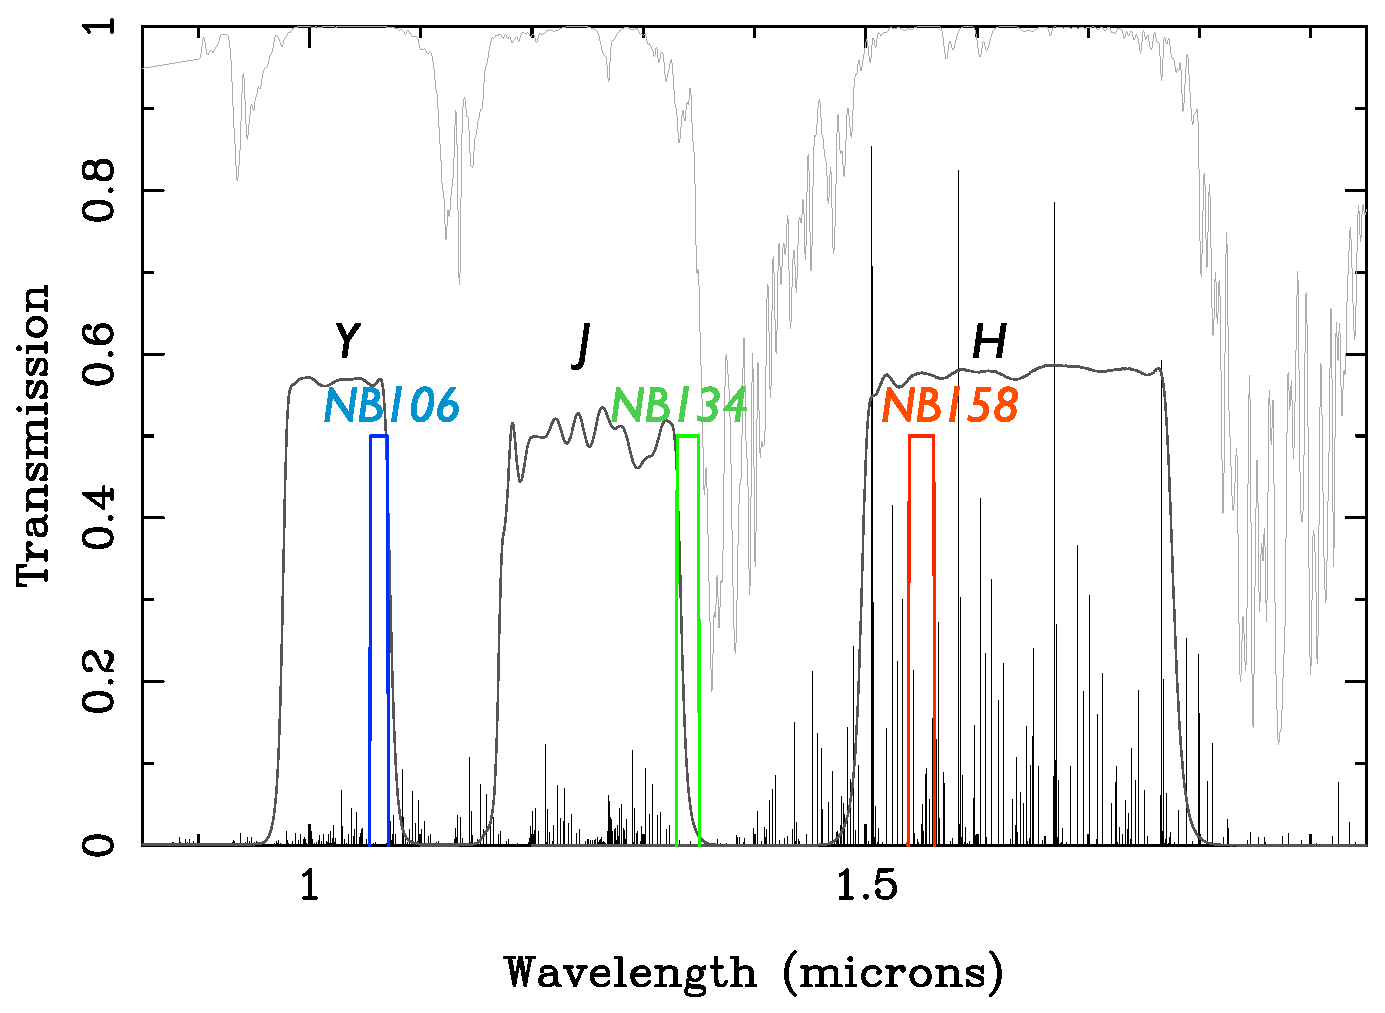
\includegraphics[width=80mm]{\thisdir figs/iwata_pg_filters_nbf01vd.eps}
}
\caption{
Transmission curves of NBFs considered. Transmission curves for $Y$,
 $J$, $H$-bands and the atomospheric transmission, and OH air glow
 strength (in arbitrary unit) are also shown.
}
\label{fig:iwata_filter_nbf}
\end{figure}

\par\noindent
[Very narrow band width filters]


\par\noindent
[What should be clarified with ULTIMATE-SUBARU.]

\subsection{Proposed Observations}

\par\noindent
[Target objects: sample selection, number of objects, number of observing
fields, sky area.]

\par\noindent
[Observing modes: imaging or spectroscopy.]

\par\noindent
[Required observing time:]

\par\noindent
[Special requirements for ULTIMATE-SUBARU other than baseline
specifications, if any.]

\subsection{Synergy and Competitions}

\subsubsection{Synergy with TMT}

\subsubsection{Competitions with other facilities}

Instruments for 8--10m class telescopes.

ELT instruments.

Space-based projects.

\bibliographystyle{apj}
\bibliography{\thisdir nbf}

\include{science/koyama/ykoyama}
\include{science/saito/saito}
\include{science/imanishi/ImanishiSJ}
\include{science/shibuya/shibuya}
\include{science/yasui/yasui}
\include{science/chiba/chiba}
\include{science/nishiyama/nishi}
\include{science/pyo/pyo}
\include{science/fukagawa/fukagawa}
\include{science/iwata/sci_summary} %\section{Science Summary: System Requirements}

%%% AO Simulation
%%%%%%%%%%%%%%%%%%%%%%%%%%%%%%%%%%%%%%%%%%%%%%%%%%%%%%%%%%%%%%%%%%%%%%%%%
% NGAO$B%o!<%/%7%g%C%WJs9p=q(B                                              %
%%%%%%%%%%%%%%%%%%%%%%%%%%%%%%%%%%%%%%%%%%%%%%%%%%%%%%%%%%%%%%%%%%%%%%%%%
%\documentclass[10pt]{jarticle}
%\usepackage{graphicx}

%\oddsidemargin   -0.25cm
%\evensidemargin  -0.25cm
%\topmargin       -0.25cm
%\textwidth        16.5cm
%\textheight       24.0cm
%\parindent        10pt

%%%%% OYA's personal new commands %%%%%
\newcommand %%%% \protect is necessary for captions %%%%%
{\supstar}{\!\!\mbox{\protect\raisebox{1.5ex}{$\star$}}}
\newcommand{\gtrsim}{\ ^{\displaystyle >}_{\displaystyle \sim}\ }
\newcommand{\lesssim}{\ ^{\displaystyle <}_{\displaystyle \sim}\ }
\newcommand{\adeg}{\hbox{$\,^{\circ}$}}
\newcommand{\arcs}{\hbox{$\,^{\prime\prime}$}}
\newcommand{\arcm}{\hbox{$\,^{\prime}$}}

\def\thisdir{simulation/glao/}

%\begin{document}

\chapter{Next-Generation AO Simulation Study
\label{chap:simulation}}

$BK\>O$G$O$9$P$kK>1s6@<!@$Be9-;kLnJd=~8w3X7O$N$?$a$N(B
$B%7%_%e%l!<%7%g%s$K4p$E$/8!F$7k2L$r$^$H$a$k!#(B
$BJd=~8w3XAuCV(B(AO: Adaptive Optics)$B$N;kLn$r9-$2$k$?$a$K$O!"(B
$BBg5$$f$i$.$N(B3$B<!859=B$$r9MN8$9$kI,MW$,$"$j!"$3$N5;=Q$r%H%b%0%i%U%#!<$H8F$V!#(B
$B%H%b%0%i%U%#!<5;=Q$r4QB,L\E*$K1~$8$F<BAu$9$k$3$K$J$k$,!"$=$NJ}<0$K$OJ#?t(B
$B$"$k(B(\ref{sec:various_ao_systems}$B@a;2>H(B)$B!#(B
$B$=$NCf$G(B
$BCOI=AXJd=~8w3X7O(B(GLAO: Ground-Layer Adaptive Optics)$B$H(B
$BB?E7BNJd=~8w3X7O(B(MOAO: Multi-Object Adaptive Optics)
$B$KBP$7$F%7%_%e%l!<%7%g%s$K$h$k8!F$$r9T$C$?!#(B

$B$9$P$kK>1s6@$K<!@$Be9-;kLn(BAO$B$rMQ$$$?@V30@~4QB,AuCV$,(B
$B3hLv$7;O$a$k:"$K$O!"8}7B(B30m$BK>1s6@$b;OF0$9$k$H4|BT$5$l$k!#(B
$B$9$P$kK>1s6@$N>-Mh7W2h$r9M$($k>e$G$O!"(B
$BL\;X$9%5%$%(%s%9$H$=$l$r<B8=$9$k5;=Q$H$$$&N>LL$K$*$$$F(B
30m$BK>1s6@$H$NAjJd@-$"$k$$$O(B30m$BK>1s6@$X$NH/E8$r0U<1$;$6$k$r$($J$$!#(B
GLAO$B$H(BMOAO$B$H$$$&(B2$B$D$N9-;kLn(BAO$B$NJ}<0$b$3$NMM$JGX7J$rF'$^$($F(B
$B%7%_%e%l!<%7%g%s$K$h$k8!F$$r?J$a$k8uJd$H$7$FA*Br$7$?!#(B
%
GLAO$B$O;kLnD>7B(B10$BJ,0J>e$H$$$&(B
$B9-;k(BAO$B$NCf$G$b:GBg$N;kLn$rC#@.$G$-$kJ}<0$G$"$k!#(B
$BJd@5@-G=$O2s@^8B3&$G$O$J$/%7!<%$%s%0$N2~A1$G$"$k$,!"(B
$B$3$N;kLn$r3h$+$9$3$H$G(B30m$BK>1s6@$HAjJdE*$J2J3XE*8&5f@.2L$,4|BT$G$-$k!#(B
$BFC$K%^%&%J!&%1%"$OBg5$$f$i$.A4BN$NCf$GCOI=AX$,@j$a$k3d9g$,Bg$-$$$3$H$,(B
$BCN$i$l$F$*$j(BGLAO$B$KE,$7$?%5%$%H$G$"$k$H8@$($k!#(B
%
MOAO$B$O9-$$;kLn$KOK$C$FF1;~$KJ#?t$NE7BN$r4QB,$9$k$3$H$G4QB,8zN($r(B
$B>e$2$k$3$H$,$G$-$kJ}<0$G$"$k!#3FE7BN$K$O2s@^8B3&$N6u4VJ,2rG=$,4|BT$G$-!"(B
$BLLJ,8w$H$NAj@-$bNI$$!#(B
MOAO$B$N<B8=$K$O?7$7$$5;=Q3+H/$,I,MW$G$"$k!#(B
$B0E$$4QB,E7BN$+$iN%$l$?J}8~$K$"$k==J,L@$k$$J#?t$NGHLL;2>H@1(B($B%,%$%I@1(B)$B$+$i!"(B
$B4QB,E7BNJ}8~$NGHLL$r?dDj$9$k%H%b%0%i%U%#!<5;=Q!"?dDj$5$l$?GHLL$r(B
$BGHLL%;%s%5(B(WFS)$B$,8+$F$$$J$$J}8~$N2DJQ7A6@(B(DM)$B$GJd@5$9$k%*!<%W%s%k!<%W@)8f5;=Q(B
$BEy$,5s$2$i$l$k!#(B
$B$9$P$kK>1s6@$K$*$$$F5;=QE*!"2J3XE*7P83$rC_@Q$7$F$$$/$3$H$G(B
30m$BK>1s6@$N<!4|4QB,AuCV$KH/E8$5$;$k$3$H$,4|BT$5$l$k!#(B

$B$3$3$G$N%7%_%e%l!<%7%g%s$O9-;kLn2=8!F$$N$?$a$G$"$k$N$G!"(B
$B$$$:$l$NJ}<0$KBP$7$F$b;kLn$r$I$3$^$G9-$/3NJ]$G$-$k$+$,(B
$B:G$b=EMW$J3NG'$9$Y$-E@$K$J$k!#(B
%
GLAO$B$N>l9g$OJd@5@-G=$,%7!<%$%s%0$K6a$$$N$G!"2s@^8B3&$r07$&0lHLE*$J(BAO$B$H$O(B
$B>u67$,0[$J$j%7!<%$%s%0$N1F6A$bBg$-$$!#(B
$B$3$N$h$&$JNN0h$G%7%_%e%l!<%7%g%s7k2L$,@5$7$$$+!"(B
$B$^$?%7!<%$%s%0%b%G%k$r$I$&Dj5A$9$k$+$KCm0U$,I,MW$G$"$k!#(B
%
MOAO$B$N>l9g$O!"8DJLE7BN$KBP$9$k9b%9%H%l!<%kHf$,L%NO$G$"$k$N$G(B
$B2s@^8B3&$N@-G=$r0];}$G$-$k;kLn$,$I$NDxEY$+!"$^$?$=$N$?$a$KI,MW$H$J$k(B
tip/tilt$B%,%$%I@1(B($BDc<!%,%$%I@1(B)$B$N?tEy$N>r7o$,CeL\$9$Y$-E@$G$"$k!#(B
%
$B$3$l$i$N9`L\$r%7%_%e%l!<%7%g%s$K$h$C$F3NG'$7$F$=$l$>$l$NJ}<0$N35MW$rGD0.$7$?(B
$B>e$G!"8!=P46EY$d%9%+%$%+%P%l!<%8$J$I$N$5$i$K>\:Y$J8!F$$X$HH/E8$5$;$F$$$/$3$H(B
$B$K$J$k!#(B

Sec.\ref{sec:gal_sim_imaging}$B$H(BSec.\ref{sec:spec_simulation}$B$G$O!"(B
GLAO$B%7%9%F%`$G$N1sJ}6d2O4QB,$,$I$N$h$&$J$b$N$K$J$k$+!"%J%A%e%i%k%7!<%$%s(B
$B%0$G$N4QB,$d2s@^8B3&$,C#@.$5$l$?>l9g$HHf3S$7$F8!F$$9$k!#(B
Sec.\ref{sec:gal_sim_imaging}$B$G$O;#A|4QB,$K$D$$$F!"(B
Sec.\ref{sec:spec_simulation}$B$G$OJ,8w4QB,$K$D$$$F$^$H$a$k!#(B



\clearpage
\begin{center}

\noindent
\Large
%%$BH/I=FbMF$N%?%$%H%k!JEvF|;H$C$?$b$N$HF10l$G$"$kI,MW$O$"$j$^$;$s!K(B
\section{Simulations of Subaru Next-Gen AO System: GLAO
\label{sec:glao_simulation}}
\vspace{0.5cm}

\noindent
\large
%%$BCx<T(B
{\bf Shin Oya$^1$}\\
$^1$ Subaru Telescope, 650 North Aohoku Place, Hilo, HI 96720, USA\\
\vspace{0.5cm}

\noindent
\normalsize
{\bf Abstract}
\end{center}
\vspace{-0.2cm}

\noindent
%abstract goes here...
$B$3$3$G$O9-;kLnJd=~8w3X7O$NCf$G$b(B10$BJ,3Q$rD6$($k:G$b9-$$;kLn$r3NJ]$G$-$k(B
$BCOI=AXJd=~8w3XAuCV(B(GLAO: Ground-Layer AO)$B$N8!F$7k2L$K4X$7$F5-=R$9$k!#(B
$B$3$NJ}<0$O>eAX$NBg5$$f$i$.$rJd@5$7$J$$$?$a!"2s@^8B3&$N@-G=$rF@$k$3$H(B
$B$G$O$J$/9-$$;kLn$K$o$?$C$F%7!<%$%s%0$r2~A1$9$k$3$H$rL\E*$H$7$F$$$k!#(B
GLAO$B$N<B8=J}K!$H$7$F$O2DJQI{6@$rF3F~$9$kJ}8~$G8!F$$r?J$a$F$$$k!#(B
$B2DJQI{6@$O(BGLAO$B0J30$K$b69;kLn$NE7BN$KBP$7$F9b$$%9%H%l!<%k$rC#@.$9$k(B
$B$3$H$,$G$-$k$N$G!"==J,L@$k$$C10l@1$KBP$9$k<+A3%,%$%I@1(B(NGS)$B4QB,!"(B
$B%3!<%s8z2L$rDc8:$9$k$?$a$NJ#?t%l!<%6!<%,%$%I@1(B(LGS)$B%H%b%0%i%U%#4QB,(B
$B$b9g$o$;8!F$$9$k$Y$-$@$H9M$($F$$$k!#(B
$B%7%_%e%l!<%7%g%s!&%3!<%I$O(BTMT$B$N(BNFIRAOS$B$N$?$a$K3+H/$5$l$?(BMAOS$B$r;HMQ$7$?!#(B



%%$BK\J83+;O!J>ON)$F$O<+M3!K(B

%%% 20130311 ommited by Iwata

%%%%%%%%%%%%%%%%%%%%%%%%%%%%%%%%%%%%%%%%%%%%%%%%%%%%%%%%%%%%%%%%%%%%%%%%%
%% NGAO$B%o!<%/%7%g%C%WJs9p=q%F%s%W%l!<%H(B
%%%%%%%%%%%%%%%%%%%%%%%%%%%%%%%%%%%%%%%%
%%
%% [AO$B$HAuCV$N;EMM(B] $B3F<+MW5a$9$k(BAO$B$dAuCV$N;EMM$r%F%s%W%l!<%H$K$"$kI=$K5-F~!#(B
%%
%% [$B;29MJ88%(B] $BI,$:L@5-$9$k$3$H!#?^$N0zMQ85$bL@5-$9$k$3$H!#(B
%%
%% [$BJ,NL(B] $B4pD49V1i(B(20$BJ,0J>e(B)$B$O(B4$B%Z!<%80J>e!"0lHL9V1i(B(15$BJ,(B)$B$O(B2$B%Z!<%80J>e!#(B
%%
%% [$BDy@Z(B] $B869FDy$a@Z$j(B 2012$BG/(B1$B7nKv(B
%%
%%%%%%%%%%%%%%%%%%%%%%%%%%%%%%%%%%%%%%%%%%%%%%%%%%%%%%%%%%%%%%%%%%%%%%%%%

%\documentclass[10pt]{jarticle}
%\usepackage{graphicx}

%\oddsidemargin   -0.25cm
%\evensidemargin  -0.25cm
%\topmargin       -0.25cm
%\textwidth        16.5cm
%\textheight       24.0cm
%\parindent        10pt

%\def\gsim{\mathrel{\raise0.35ex\hbox{$\scriptstyle >$}\kern-0.6em % Greater/squiggles
%\lower0.40ex\hbox{{$\scriptstyle \sim$}}}}
%\def\lsim{\mathrel{\raise0.35ex\hbox{$\scriptstyle <$}\kern-0.6em % Less than/squiggles 
%\lower0.40ex\hbox{{$\scriptstyle \sim$}}}}

%\begin{document}

\def\thisdir{simulation/moao/}

\begin{center}

\noindent
\Large
\section{Simulations of Subaru Next-Gen AO System: MOAO
\label{sec:moao_simulation}}
\vspace{0.5cm}

\noindent
\large
%%$BCx<T!JNc!K(B
{\bf Masayuki Akiyama$^1$}\\
$^1$ Astronomical Institute, Tohoku University, 3-6 Aramaki, Aoba-ku, Sendai, Japan
\vspace{0.5cm}

\noindent
\normalsize
{\bf Abstract}
\end{center}
\vspace{-0.2cm}

\noindent
$B$3$3$G$O$9$P$kK>1s6@$K$*$$$F(B6$B8D$N%l!<%6!<%,%$%I@1$rMQ$$$F(B
$BB?E7BNJd=~8w3X(B(MOAO)$B$r9T$C$?>l9g$KM=A[$5$l$k@-G=$r8!F$$7$?(B
$B7k2L$r$^$H$a$k!#FC$K!"(BMOAO$B$rMQ$$$k$3$H$GCO>eAXJd=~8w3X(B(GLAO)
$B$h$j$b9b$$Jd=~@-G=$r9-$$NN0h$NB?E7BN$K$D$$$F<B8=$9$k$3$H$r(B
$BL\;X$9!#$=$N$?$a(BGLAO$B$h$j$b9b$$Jd=~@-G=$r0];}$7$D$D!"$I$NDxEY(B
$B$^$G%?!<%2%C%HNN0h$r9-$2$i$l$k$N$+$rI>2A$9$k$3$H$K=EE@$r(B
$BCV$/!#(BMOAO$B$N>l9g$K$O;kLn$NCf$rO"B3E*$KJd@5$9$k$3$H$O$;$:!"(B
$BFCDj$N%?!<%2%C%H$NJ}8~$N$_$NJd@5$r9T$C$F$$$k$3$H$KCm0U$,(B
$BI,MW$G$"$k!#$=$N$?$a0J2<$G$O$3$N%?!<%2%C%H$rA*Br$9$kNN0h$N(B
$B$3$H$r%?!<%2%C%HNN0h$H8F$V!#(B6$B8D$N%l!<%6!<%,%$%I@1$rMQ$$$?(B
$B>l9g!"H>7B(B$3^{\prime}$$BDxEY$N%?!<%2%C%HNN0h$K$D$$$F$O(BGLAO
$B$h$j$b9b$$Jd=~@-G=$,4|BT$5$l$k$,!"$=$l$h$j$b%l!<%6!<%,%$%I@1$N(B
$B4V3V$r9-$2$F%?!<%2%C%HNN0h$r9-$2$k$H;kLn$N$[$H$s$I$NNN0h(B
$B$G(BGLAO$B$K6a$$Jd=~@-G=$7$+F@$i$l$:!"(BMOAO$B$N%a%j%C%H$,(B
$B@8$+$;$J$/$J$k$3$H$,$o$+$C$?!#$^$?<+A3%,%$%I@1$N4V3V$,3+$/$K$D$l(B
$B$F(B Tip-Tilt $B$NGHLL8m:9$,5^7c$KBg$-$/$J$k$3$H$b$o$+$C$?!#(B
Tip-Tilt $B%,%$%I@1$KMQ$$$k$3$H$N$G$-$k<+A3%,%$%I@1$NL@$k$5(B
$B$r9M$($k$H6d6KJ}8~$K$*$$$F$OJ#?t$N<+A3%,%$%I@1$r%?!<%2%C%H(B
$BNN0h$KMQ0U=PMh$k3NN($O$+$J$jDc$/!"(BTip-Tilt $B$NGHLL;D:9$,(B
$B@-G=$r%j%_%C%H$9$k!#(B


%%$BK\J83+;O!J>ON)$F$O<+M3!K(B

%%% 20130311 ommitted by Iwata

\include{science/minowa/minowa}
\include{science/iwata/ngao_spec_simulation}

%%% System Design
%\documentclass[10pt]{jarticle}
%\usepackage{graphicx}
%\usepackage{url}

%\oddsidemargin   -0.25cm
%\evensidemargin  -0.25cm
%\topmargin       -0.25cm
%\textwidth        16.5cm
%\textheight       24.0cm
%\parindent        10pt

%\def\gsim{\mathrel{\raise0.35ex\hbox{$\scriptstyle >$}\kern-0.6em % Greater/squiggles
%\lower0.40ex\hbox{{$\scriptstyle \sim$}}}}
%\def\lsim{\mathrel{\raise0.35ex\hbox{$\scriptstyle <$}\kern-0.6em % Less than/squiggles 
%\lower0.40ex\hbox{{$\scriptstyle \sim$}}}}

\def\thisdir{development/design/}

%\begin{document}

\chapter{System Study for Subaru Next-Generation AO
\label{chap:system_design}}

\section{Comparisons of Candidate AO Systems for Subaru Telescope
 Next-Generation AO
\label{sec:various_ao_systems}}

%%% 20130311 ommited by Iwata

\section{Overview of the System}

%%% 20130311 ommited by Iwata.
%%% Need to include overview of NIR instrument(s) as well?

$B8=;~E@$G5DO@$,?J$a$i$l$F$$$k<!@$Be(BAO$B$*$h$S@V30@~AuCV$N(B
$B4pK\;EMM$rI=(B\ref{tab:spec}$B$K<($7$?!#$3$N;EMM$O:#8e$N>\:Y$J(B
$B8!F$$K$h$C$F$OBgI}$KJQ99$5$l$k2DG=@-$,$"$k!#(B
\begin{table}[t]
\begin{center}
\begin{tabular}{|l|l|l|l|l|}
\hline
 Item & Specification \\
 \hline
 $B4QB,GHD90h(B & 0.9--2.5 $\mu$m ($B%5%$%(%s%9(BWS$B$+$i$NMW5a$O(B0.6--5$\mu$m\\
 $B4QB,%b!<%I(B & $B;#A|!"J,8w!JLLJ,8w$r9MN8$9$k!K(B\\
 $B4QB,;kLn(B & $\phi$ 15$BJ,3Q!J(B20$BJ,3QL\I8!K(B\\
 $B>GE@0LCV(B & $B%+%;%0%l%s>GE@(B \\
 \hline
 $B%,%$%I@1(B & 4 LGS$B!"(BNGS$B!J(B2$\sim$4$B8D$+!)!K(B\\
 $B%,%$%I@1$NA*BrHO0O(B & LGS$B$O4QB,;kLn$NC<!"(BNGS$B$O4QB,;kLnFb(B \\
 $BGHLL%;%s%5!<(B & $B%,%$%I@1$K$=$l$>$l(B1$B$D$:$D(B (Guide star oriented)\\
 $BGHLL%;%s%5!<%?%$%W(B & $B%7%c%C%/%O%k%H%^%s7?!J%T%i%_%C%I7?$bMW8!F$!K(B \\ 
 $BGHLL%;%s%5!<AG;R?t(B & 100$BDxEY$+$=$l0J>e(B ($B9b%9%H%l!<%k$J$i(B1000$BAG;RDxEY$b(B) \\
 $BGHLL%;%s%5!<%5%s%W%j%s%0<~GH?t(B & 500Hz$B0J>e!J(BGLAO$B$O(B100Hz$B$G$b2D!K(B \\
 $B2DJQ7A6@(B & $BI{6@$r2DJQ7A6@2=(B \\
 $B2DJQ7A6@AG;R?t(B & 500$\sim$1000$BDxEY(B \\
 $BGHLL@)8f%b!<%I(B & GLAO (LTAO$B!"(BExAO$B$J$I$X$N@ZBXBP1~$,I,MW$+!)(B)\\
 \hline
\end{tabular}
\caption{$B<!@$Be(BAO$B$*$h$SAuCV$N4pK\;EMM0F(B}
\label{tab:spec}
\end{center}
\end{table}

\section{Technical Challenges}

$B>e=R$7$?(BTomography AO$B$K6&DL$9$k5;=QE*$J2]Bj$O!"(B
$B%l!<%6!<5;=Q$*$h$SJ#?t%l!<%6!<%,%$%I@1$N@=:n5;=Q!"(B
$BBg5$$f$i$.$N9b$5J}8~$N(Btomography$B?dDj5;=Q!"(B
$B2DJQI{6@!"@)8f7W;;5!$J$I$,$"$k!#(B
$B$?$@$7!"@$3&$ND,N.$H$7$F(Btomography AO$B$O@9$s$K(B
$B%7%9%F%`8!F$!"5;=Q8!F$$,?J$a$i$l$F$*$j!"(B
$B5;=QE*$J2]Bj$O$+$J$j9nI~$5$l$D$D$"$k$N$,8=>u$G$"$k!#(B

$B=i4|$N%l!<%6!<%,%$%I@1$O?'AG%l!<%6!<$,<gBN$G$"$C$?!#(B
$B$3$l$O%l!<%6!<G^<A$,1UBN$G$"$j!"0BDj@-!"J]<i@-$K(B
$BBg$-$JO+NO$,I,MW$G$"$k!#$^$??'AG$NNt2=$K$h$k=PNODc2<$,(B
$BHr$1$i$l$J$$!#<!$KH>F3BN%l!<%6!<$H%l!<%6!<7k>=$N(B
$B5;=QH/E8$,$"$j!"8GBN%l!<%6!<$,BfF,$7$F$/$k!#(B
$B:#$G$O%J%H%j%&%`AX$rNe5/$9$k$?$a$NOB<~GHH/@8$rMQ$$$?(B
$BA48GBN%l!<%6!<$,5;=QE*$K@.=O$7$F$-$?!#(B
Gemini$B$N(BMCAO$B$G$O=PNO(B50W$B$N%l!<%6!<$r(B5$B$D$KJ,3d$7$F!"(B
5$B8D$N%J%H%j%&%`%l!<%6!<%,%$%I@1$N:n@.$K@.8y$7$F$$$k!#(B
$B0lJ}!"%U%!%$%P!<%l!<%6!<5;=Q$rMQ$$$?%3%s%Q%/%H$+$D(B
$B0BDj$7$?%l!<%6!<$N3+H/$,(BESO$B$rCf?4$K?J$a$i$l!"(B
$B%I%$%D$N(BTOPTICA$B<R$H%+%J%@$N(BMPB$B<R$N6&F1$G(B
$BO"B3GH(B20W$B$N%l!<%6!<$,@=IJ2=$5$l$?!#(B
$B$3$N%l!<%6!<$OB>$N(B8m$B%/%i%9$N<!@$Be(BAO$B$*$h$S(B
ELT$BMQ(BAO$B$N%l!<%6!<%,%$%I@1MQ8w8;8uJd$H$7$FBg$-$J(B
$B4|BT$,4s$;$i$l$F$$$k!#2f!9$b$9$G$K(BMPB$B<R$H(B
$BHkL)J];}7@Ls$rDy7k$7!"5;=Q>pJs$N8r49!"(B
$B4pK\;EMM$N8!F$=`Hw$r?J$a$F$$$k!#(B
$B$^$?!"%l%$%j!<;6Mp$rMxMQ$7$?%l!<%6!<%,%$%I@1$b(B
WHT$B!"(BMMT$B$J$I$GCOF;$K;n83$,B3$1$i$l$F$$$k!#(B
8m$B%/%i%9$N(Bsingle conjugate $B%l!<%6!<%,%$%I@1(BAO$B$,(B
$B0BDj$7$F1?MQ$5$l$F$*$j!"%l!<%6!<%,%$%I@1$K(B
$B4X$9$k4pAC5;=Q!"1?MQ5;=Q$O$*$*$$$K?JJb$7$?!#(B
$B%l!<%6!<%7%9%F%`$K$D$$$FI=(B\ref{tab:Laser}$B$K$^$H$a$?!#(B

\begin{table}[t]
\begin{center}
\begin{tabular}{|l|l|l|l|l|l|l|l|}
\hline
 %$BK>1s6@(B & Subaru & Keck I & Keck II & Gemini N & VLT  & Gemini S & LBT \\
% \hline
%$B%l!<%6!<%,%$%I@1(B & Na$BAX(B & Na$BAX(B & Na$BAX(B & Na$BAX(B. & Na$BAX(B  & Na$BAX(B & $B%l%$%j!<;6Mp(B \\
%$B%l!<%6!<%?%$%W(B & $BOB<~GH(B & $BOB<~GH(B & $B?'AG(B & $BOB<~GH(B. & $B?'AG(B->$B%U%!%$%P!<(B  & $BOB<~GH(B & $BA48GBN%0%j!<%s(B \\
%$B%l!<%6!<G^<A(B & $B8GBN7k>=(B & $B8GBN7k>=(B & $B?'AGM-5!1UBN(B & $B8GBN7k>=(B. & $B?'AGM-5!1UBN(B->$B8w%U%!%$%P!<(B  & $B8GBN7k>=(B & $B8GBN7k>=(B \\
%$B=PNO(B & $\sim$6W & $\sim$40W & $\sim$15W & $\sim$15W & $\sim$10W->$\sim$25W & $\sim$10W / beacon & $\sim$18W / beacon \\
%$B%l!<%6!<H/?67ABV(B & 143MHz & 75MHz & 13kHz or 26kHz & 75MHz & $BO"B3GH(B & 75MHz & 10kHz \\
$B%,%$%I@1%?%$%W(B & \multicolumn{3}{|c|}{$B%J%H%j%&%`AX(BLGS} &  \multicolumn{1}{|c|}{$B%l%$%j!<(BLGS} \\
\hline
$B%l!<%6!<%?%$%W(B & $B?'AG(B & $BA48GBNOB<~GH(B & $B8w%U%!%$%P!<%l!<%6!<(B & $BA48GBN!!(B\\
\hline
$B%l!<%6!<G^<A(B & $B1UBNM-5!MOG^(B & $B8GBN7k>=(B & $B8w%U%!%$%P!<(B& $B8GBN7k>=(B \\
\hline
$BK>1s6@(B & Keck II & Subaru, Keck I & VLT$B!J<!@$Be!K(B & LBT \\
             & VLT & Gemini N\&S &       &  (Na-LGS$B$b7W2hCf(B) \\
\hline
$B=PNO(B & 15W(Keck II) & 6W(Subaru) & 25W(VLT$B<!@$Be(B) & 18W$\times$3 (LBT) \\
    &    &  40W(Keck I) & & \\
    &  10W(VLT) & 15W(GeminiN) & &  \\
    &    &  10W$\times$5 (GeminiS) & & \\
\hline
$BH/?67ABV(B & 26kHz(Keck II) & 143MHz(Subaru) & $BO"B3GH(B(VLT$B<!@$Be(B) & 10kHz(LBT) \\
  & $BO"B3GH(B(VLT) & 75MHz(Keck I) & & \\
  &   & 75MHz(Gemini N\&S) & & \\
\hline
\end{tabular}
\caption{$B%l!<%6!<%,%$%I@1MQ%l!<%6!<%7%9%F%`$NHf3S(B}
\label{tab:Laser}
\end{center}
\end{table}


$B:GBg3QEY$G$b(B10$BJ,3Q$H$$$&69$$HO0O$N8w8;$rMQ$$$F!"(B
$BESCf$K$"$kBg5$$f$i$.$N(B3$B<!85J,I[$r?dDj$9$k(B
tomography$B?dDj5;=Q$O!"0lHL$N(B3$B<!85(Btomography$B$H$O(B
$B$+$J$j0[$J$kMWAG$r4^$s$G$$$k!#$7$+$7!"B?$/$N(B
AO tomography$B%"%k%4%j%:%`$,Ds>'$5$l!"7W;;5!(B
$B%7%_%e%l!<%7%g%s!"%F%9%H%Y%C%I$K$h$k<B83$,(B
$B?J$a$i$l$F$-$?!#>\:Y$J8!F$$*$h$S%7%9%F%`$KFC2=$7$?(B
$B8!F$$O$^$@I,MW$G$"$k$,!"4pACE*$J(BAO tomography$B$N(B
$B8&5f$O==J,$J$5$l$F$-$F$$$k!#$9$P$k<!@$Be(BAO$B8!F$(B
$B%o!<%-%s%0%0%k!<%W$O!":#8e>\:Y8!F$$rB3$1$F$$$/M=Dj$G$"$k!#(B

$BFC$K(BGLAO$B$O2DJQI{6@$,=EMW$J%3%s%]!<%M%s%H$H$J$k!#(B
$BF|K\$G$O$^$@2DJQI{6@$N8!F$$O?J$a$i$l$F$$$J$$$,!"(B
$B%"%j%>%J$N(BMMT$B!"(BLBT$B$G$O$9$G$K2DJQI{6@$,Ek:\$5$l!"(B
$BL@$k$$%,%$%I@1$G$h$$Jd@5@-G=$rC#@.$7$F$$$k!#(B
$B$^$?%A%j$N(BVLT$B$N$?$a$N2DJQI{6@$,@=:nCf$G$"$k!#(B
$B$3$l$i$N2DJQI{6@$r@=:n$7$?$N$O%$%?%j%"$N(BMicrogate$B<R$G$"$k!#(B
$B2f!9%o!<%-%s%0%0%k!<%W$O$9$G$K(BMicrogate$B<R$H%3%s%?%/%H$r$H$j!"(B
$B$9$P$kK>1s6@MQ$N2DJQI{6@$N35G08!F$$N=`Hw$r?J$a$F$$$k!#(B

$BJ#?t$N%,%$%I@1!"J#?t$"$k$$$OB?AG;R$N2DJQ7A6@$r@)8f$9$k$?$a$N(B
$B7W;;5!$KMW5a$5$l$k@-G=$OHs>o$K9b$$!#2f!9%o!<%-%s%0%0%k!<%W$O!"(B
$B$^$@@)8f7W;;5!$N8!F$$r;O$a$F$$$J$$$,!"(BTMT$BMQ$N%U%!!<%9%H%i%$%H(BAO
$B$G$"$k(BNFIRAOS$B$N@)8f7W;;5!8!F$$,==J,;29M$K$J$k$H9M$($F$$$k!#(B

\section{Interfaces with the Subaru Telescope -- 20130311Iwata: to be ommitted?}

$B$9$P$kK>1s6@<!@$Be(BAO$B$NBh0l8uJd$G$"$k(BGLAO$B$K$D$$$F!"(B
$BK>1s6@$H$N%$%s%?!<%U%'!<%9$r9M;!$7$?!#(B
GLAO$B$N:GBg$NFCD'$O!"2DJQI{6@$rMQ$$$F$$$k$3$H$G!"(B
$BH?<MLL$,>/$J$/8zN($,9b$$$3$H$,$"$2$i$l$k!#(B
$B=>$C$F!"4QB,AuCV$O%+%;%0%l%s>GE@$K@_CV$9$k$N$,$h$$!#(B
$B$^$?!"(BGLAO$B$G$O(B10$BJ,3Q$rD6$($k;kLn$,L%NO$H$J$C$F$$$k!#(B
$B8=:_;H$o$l$F$$$k%+%;%0%l%s>GE@$N2D;kMQBg5$J,;6Jd@58w3X7O$O(B
$B$=$3$^$G$N;kLn$r3NJ]$G$-$F$$$J$$!#(BGLAO$B$H6a@V30@~4QB,AuCV$N(B
$BAH$_9g$o$;$N$H$-$OBg5$J,;6Jd@58w3X7O$O<h$j30$9I,MW$,$"$k!#(B

$B%+%;%0%l%s>GE@$N4QB,AuCV$N8!F$$b=EMW$G$"$k!#(B
GLAO$B$N9-;kLn$r@8$+$96a@V30@~;#A|J,8wAuCV$r8!F$$9$k>e$G!"(B
$BK>1s6@$N8w3X<}:9!"AuCV$N%5%$%:!"=ENL!"@_7W@=B$2DG=$J8w3X7O$N@_7W(B
$B$J$I$,=EMW$J%U%!%/%?!<$H$J$k!#(B

$B2DJQI{6@$O$9$P$kK>1s6@$N%H%C%W%f%K%C%H$K@\B3$5$l$k!#(B
$B$9$P$kK>1s6@$O<g>GE@It$K9-;kLn%+%a%i$J$I$r(B
$BEk:\$9$k$?$a!"%H%C%W%f%K%C%H8r495!$N=ENL@)8B$,(B
3t$B$G$"$k!#8=:_@=:nCf$N(BVLT$BMQ2DJQI{6@$NAm=ENL$O(B1500kg
$BDxEY$J$N$G7ZNL2=$NEXNO$OITMW$G$"$k!#(B
$B8=:_;HMQCf$N@V30I{6@$OD>7B$,(B1265mm$B$G$"$j!"(B
VLT$B$N2DJQI{6@D>7B$h$j$b<c43Bg$-$$!#(B
$B%+%;%0%l%s>GE@$N(BF$BCM$NJQ99$b9MN8$7$?2DJQI{6@$N;EMM:vDj$r(B
$B:#8e?J$a$F$$$/$3$H$K$J$k!#(B
$B%H%C%W%f%K%C%H$K$*$1$kEENO6!5k!"@)8f@~!"%M%C%H%o!<%/!"Nd5Q?e(B
$B$J$I$N4pK\E*$J%$%s%U%i!"%H%C%W%f%K%C%H$H$N%$%s%?!<%U%'!<%9!"(B
$B$J$I$N8!F$$b=EMW2]Bj$G$"$k!#(B

\section{Subaru GLAO System Structure}


%%% 20130311 ommitted by Iwata

%%% 20130311 additions by Iwata
\section{Components of GLAO: Adaptive Secondary Mirror}

\section{Components of GLAO: Wavefront Sensing System}

\section{Components of GLAO: Laser System}

\section{Components of GLAO: RTC}

%%% 20130311 additions by Iwata
\section{Telescope Modifications}

\subsection{Top Unit}

\subsection{Cassegrain Focus}

\subsection{Other Areas?}



\section{Operations of GLAO}

$B$9$P$kK>1s6@$O<g>GE@4QB,AuCV$,$"$k$?$a!"2DJQI{6@$r>o@_$9$k$3$H$O(B
$B1?MQ>e$G$-$J$$!#$=$N$?$a!"2DJQI{6@$O%H%C%W%f%K%C%H8r49AuCV$r(B
$BMQ$$$FCeC&$9$kI,MW$,$"$k!#$=$N$?$a$N%$%s%?!<%U%'!<%9;EMM$r(B
$B3NDj$7$J$1$l$P$J$i$J$$!#$^$?2DJQI{6@$NIT;HMQ;~$NJ]4I>l=j$N3NJ]$H(B
$B$=$N%$%s%?!<%U%'!<%9$H%$%s%U%i$N;EMM$K$D$$$F$b7h$a$kI,MW$,$"$k!#(B
$B$^$?!"8r49;~$N4D6->r7o!"?6F0>r7o!"6@$NJ];}$"$k$$$O0BA4$J>uBV4IM}$K(B
$B$D$$$F$b8!F$$rMW$9$k!#(B

$B0lJ}!"$9$P$kK>1s6@$NI{6@$OFLLL$G$"$k!#FLLL$N2DJQI{6@$N%-%c%j%V%l!<%7%g%s(B
$BJ}K!$K$D$$$F$b8!F$$,I,MW$@!#$^$?!"2DJQI{6@$N:F>xCe$NI,MW@-!"Dj4|E*$J(B
$BJ]<i9`L\$J$I$b=i4|8!F$$NCJ3,$G5DO@$7$F$*$/$Y$-$G$"$m$&!#(B

$B%l!<%6!<<M=P%7%9%F%`$O!"K>1s6@$N%;%s%?!<%;%/%7%g%s$K>o@_$9$k$3$H$r(B
$B8!F$Cf$G$"$k!#CeC&$NI,MW@-$O$J$$$,!"%l!<%6!<$NJ]<i!"ItIJ$N8r49!"(B
$B7PG/JQ2=$X$NBP1~!"0BA44IM}$r4^$a$?%l!<%6!<1?MQBN@)$OI,?\$H$J$k!#(B

$BGHLL%;%s%5!<$O%+%;%0%l%s>GE@>eIt$N%+%;%0%l%s%U%i%s%8$H8F$P$l$kCf$K(B
$B@_CV$5$l$k!#$3$NItJ,$O%"%/%;%9$,BgJQFq$7$/!"AuCV$N8N>c!"2~=$$,(B
$BFq$7$$!#$=$N$?$a$N7xO4!"J]<iITMW$NGHLL%;%s%5!<%7%9%F%`8!F$$OBg@Z$G$"$m$&!#(B

\section{Perspective of Future Development}

GLAO$B%7%9%F%`$O<g$H$7$F2DJQI{6@!"%+%;%0%l%s%U%i%s%8$NGHLL%;%s%5!<!"%l!<%6!<(B
$B<M=P7O!"4QB,AuCV$H$$$&9=@.$+$i$J$k!#$3$N%3%s%]!<%M%s%H$OB>$N(BAO$B%7%9%F%`$K(B
$B$H$C$F$b=EMW$J9=@.MWAG$G$"$k!#(B

$B2DJQI{6@$NAG;R?t$O(B1000$BDxEY$H$J$k8+9~$_$G$"$k!#$=$N$?$a!"L@$k$$<+A3%,%$%I@1MQ$N(B
$BGHLL%;%s%5!<$r4QB,AuCVB&$KMQ0U$9$k$H!"%+%;%0%l%s!"%J%9%_%9$N$$$:$l$N>GE@$K$b(B
Extreme AO$BAuCV$,$G$-$k!#$b$A$m$s!"8=B8$"$k$$$O7W2hCf$N9b%3%s%H%i%9%H4QB,AuCV$K$b(B
$B1~MQ$,$G$-$k$G$"$m$&!#2DJQI{6@$OCf4V@V30@~$NAuCV$NGX7J8w$r2!$5$($kMxE@$H$b$J$k!#(B

$B$^$?!"J#?t%l!<%6!<<M=P7O$O(BMOAO$B$KMxMQ$G$-!"2DJQI{6@$O(BMOAO$B$N(Bwoofer$B$H$7$F;HMQ$7!"(B
$B4QB,AuCVB&$K(BMOAO$B$N(Btweeter$B2DJQ7A6@$r$b$?$;$k$3$H$G!"8zN($NNI$$AuCV$,9M0F$G$-$k$G$"$m$&!#(B

$B$3$N$h$&$K(BGLAO$B%7%9%F%`$OK>1s6@5!G=$N%]%F%s%7%c%k$NDl>e$2$r$9$k$b$N$G$"$k!#(B

%\end{document}


%%% Instruments
%\chapter{Instruments for Subaru Next-Generation AO}
\def\thisdir{instrument/}

\chapter{Instruments for Subaru Next-Generation AO
\label{chap:inst}}


\section{Requirements on Instrument from Scientific Objectives}

Here we re-summarize the requirements from key science cases on
instrument specifications.

\begin{itemize}
 \item Field of view
 \item Pixel scale
 \item Requirements on broad-band filters (numbers, wavelength coverages)
 \item Requirements on narrow-band filters (numbers, spectral resolution,
      wavelength uniformity, wavelength coverages)
 \item Spectroscopy: Spectral resolution 
 \item Requirements on multi-object spectrograph mode
\end{itemize}

In this chapter we summarize the studies we have made so far on
instruments for ULTIMATE-SUBARU.

\def\thisdir{instrument/optics/}

\begin{center}
\section{Studies of the Optics for the Wide-Field Near-IR Imager and
 Multi-object Spectrograph
\label{sec:inst_optics}}
\vspace{0.5cm}

\noindent
\large
%% authors
{\bf T. Yamamuro$^{1}$, K. Motohara$^{2}$, I. Iwata$^{3}$ and Subaru
Telescope Next-Gen AO Instrument sub-working group}\\
$^1$ Optocraft
$^2$ Institute of Astronomy, University of Tokyo
$^3$ Subaru Telescope, National Astronomical Observatory of Japan
\vspace{0.5cm}

\end{center}

Here we summarize results of studies made by Dr. Yamamuro (Optcraft).
Document Number: CP0046--11--RP001 (w/o FoV split), CP0046--12--RP001 (w
FoV split).

\subsection{Optical Design without FoV Split}

First we studied how wide field of view can be achieved at the
Cassegrain focus of Subaru Telescope with the following conditions:

\begin{itemize}
 \item Single set of optics can be used (i.e., no FoV split is
       considered).
 \item We consider a near-infrared camera and spectrograph. Wavelength
       range is from 0.8$\mu$m to 2.5$\mu$m. The optics will be cooled
       down to about 100K.
 \item The target image quality is to achieve FWHM $<0.15''$ over the
       entire FoV in all of $J$, $H$, $K$-bands.
 \item The focal plane of the instrument should be flat so that we can
       achieve the above image quality by using science detectors with
       flat pixel arrays.
 \item The use of Teledyne H4RG (15$\mu$m pixel size) is assumed.
 \item The sizes of optical components should be feasibile; for example,
       the maximum size of components made of CaF$_2$ and BaF$_2$ should
       be less than 40cm.
\end{itemize}

We examined the two cases on the telescope parameters; (A) the case we
use the existing optical parameters of Subaru Telescope and (B) the case
with new parameters for the secondary mirror and also that the shape of 
primary mirror can be adjusted within the range of the stroke which the
existing mirror actuators are achievable.

Also, we should consider the necessity of field flatner for the
telescope focus. In order to achieve multi-object spectroscopy (MOS), we
need to insert a mask with slitlets at the telescope focus. Since the
Cassegrain focal plane has a curvature, in order to enable the use of
flat MOS mask, we need to insert field flatning lens(es). For the case
A, we show both the case with and without field flatner.

\subsubsection{A. Cases in which Subaru Telescope optical parameters are
   not changed}

Here we show the simplest case where there is no change in the telescope 
parameters and no field flatner is included.
Fig.\ref{fig:optcraft_fig01} is the optical layout. It consists of nine
collimator lenses and seven camera lenses. Lense materials are CaF$_2$, 
BaF$_2$, Fused silica, and ZnSe.The last lens of the camera section is
aspherical. 

\begin{figure}[!ht]
\centerline{
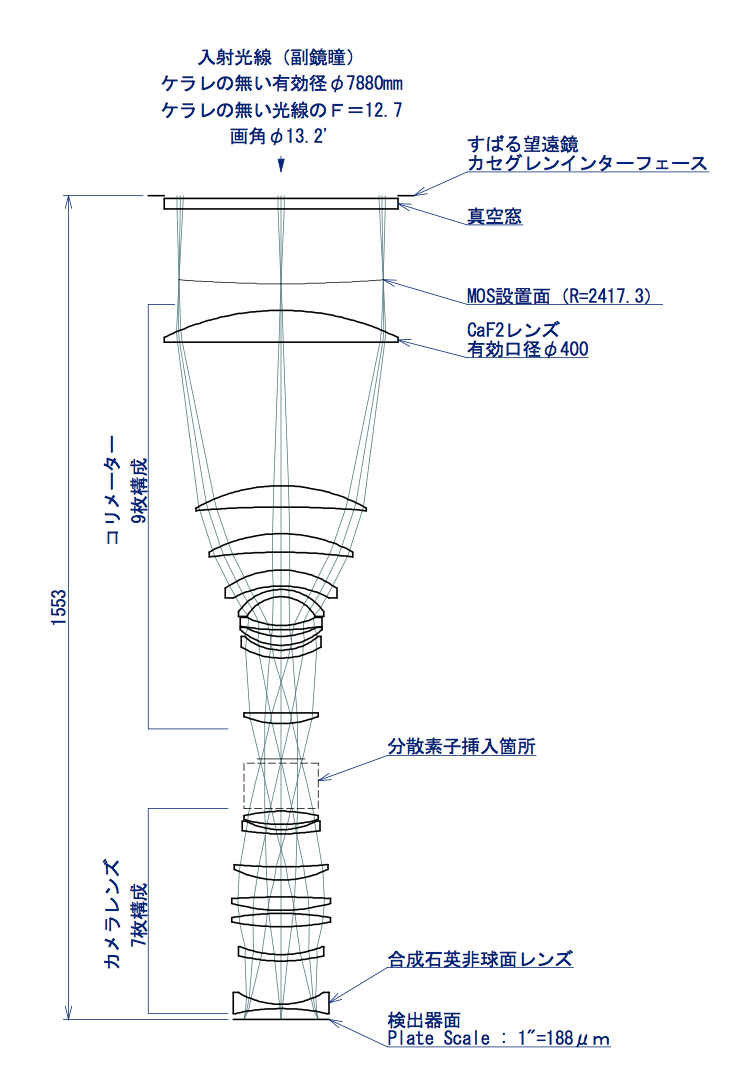
\includegraphics[width=120mm]{\thisdir figs/optcraft_fig01.eps}
}
\caption{Optical layout for Case A: no change in the telescope
 parameters. The case without field flatner.
}
\label{fig:optcraft_fig01}
\end{figure}

The field of view is determined so that the size of effective beam for
the largest lens is within $\phi$400mm, and in this solution it is 
$\phi 13.2'$. The effective diameter of the primary mirror is 
$\phi 7.88$m to achieve the above FoV at the secondary mirror pupil and
to block the light outside of the primary mirror (physical size 
$\phi$8.2m). Since this layout does not include field flatner, the
telescope focal plane has a curvature, and there is astigmatism.

The spot diagram at the position of the MOS mask (with a radius of
curvature of 2417.3mm) is shown in
Fig.~\ref{fig:optcraft_fig02}(left). The degradation of the image toward
the edge of FoV ($\sim 0.2''$ at the edge) is due to astigmatism. 
In this case the slit width at the edge should be adjusted to this image
quality. 
Fig.~\ref{fig:optcraft_fig02}(right) shows the size of distortion at the
position of the MOS mask.

\begin{figure}[!ht]
\centerline{
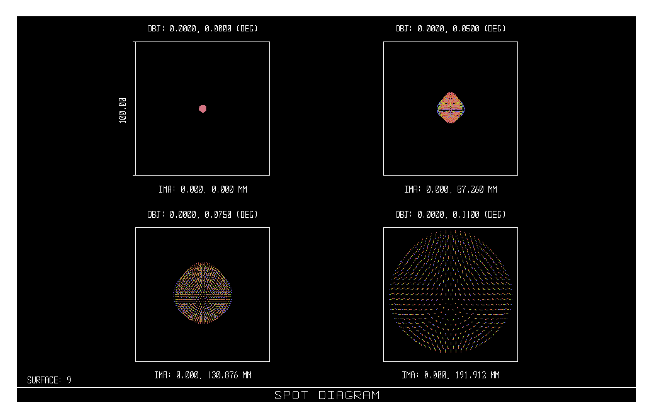
\includegraphics[width=100mm]{\thisdir figs/optcraft_fig02.eps}
 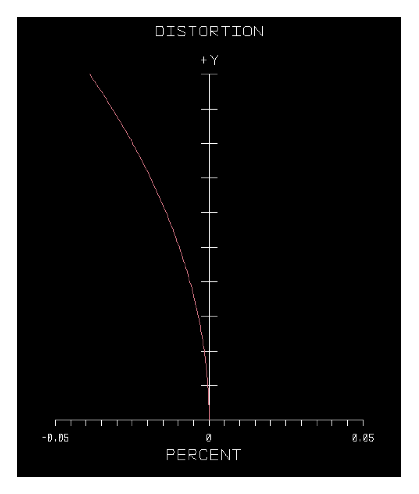
\includegraphics[width=60mm]{\thisdir figs/optcraft_fig03.eps}
}
\caption{(Left) Spot diagram at the position of the MOS mask with a
 curvature radius of 2417.3mm for a configuration shown in 
Fig.\ref{fig:optcraft_fig01}. Spot diagrams with wavelengths from
 0.8$\mu$m to 2.5$\mu$m are shown altogether, as wavelength dependence
 is small. (Right) distortion at the
 position of the MOS mask. The value is $-0.04$\% at the edge.
}
\label{fig:optcraft_fig02}
\end{figure}

The spot diagram and distortion at the position of the detectors are
shown in Fig. \ref{fig:optcraft_fig04}. All FWHM values are smaller than
the target FWHM (0.15$''$) except the case with 0.8$\mu$m
at the edge ($6.6'$) in which the FWHM is slightly larger than
0.15$''$. However, the distortion is large; at the edge it is 
$-6.3$\%.

\begin{figure}[!ht]
\centerline{
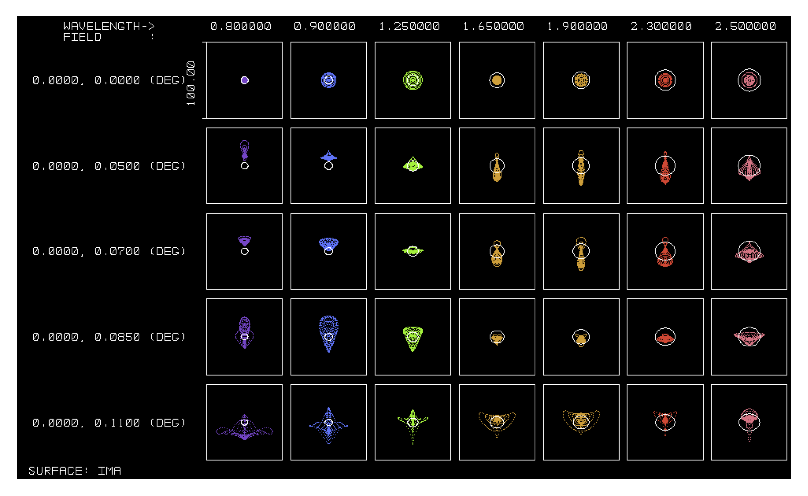
\includegraphics[width=120mm]{\thisdir figs/optcraft_fig04.eps}
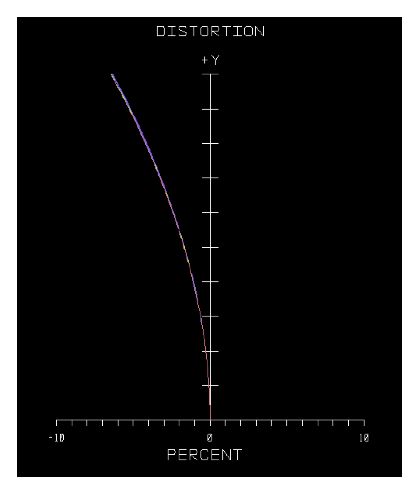
\includegraphics[width=60mm]{\thisdir figs/optcraft_fig05.eps}
}
\caption{(Left) Spot diagram at the position of the detectors for a
 configuration shown in Fig.\ref{fig:optcraft_fig01}.
Five positions from 0$'$ (center) to 6.6$'$ (edge) are shown along the
 vertical axis, and the cases with wavelengths from 0.8$\mu$m to
 2.5$\mu$m are plotted along the horizontal axis. 
The box size is 100$\mu$m which corresponds to 0.53$''$.
(Right) Distortion at the position of the detectors.
}
\label{fig:optcraft_fig04}
\end{figure}


We also evaluated the performance in spectroscopy. As a preliminary
analysis, here we only examined the image quality in spectroscopy in the
range 0.8--2.5$\mu$m without order-sorting.
Fig.~\ref{fig:optcraft_fig06} shows the positions of images in
spectroscopy as a function of wavelength.
Here we assume a fused silica grism with 160 grooves/mm, blaze angle 
34$\circ$\footnote{In section ** we examine more details of various
grisms}.
Fig.~\ref{fig:optcraft_fig07} is the spot diagram. Image qualities at
the shorter and longer wavelength edges and at the edge of FoV is not
good; in 2.5$\mu$m and at $6.6'$ from the center the RMS spot diameter
is $0.22''$. However, it is $0.17''$ at $5.5'$ from the center, and
at the other positions the image quality meets the goal.

\begin{figure}[!ht]
\centerline{
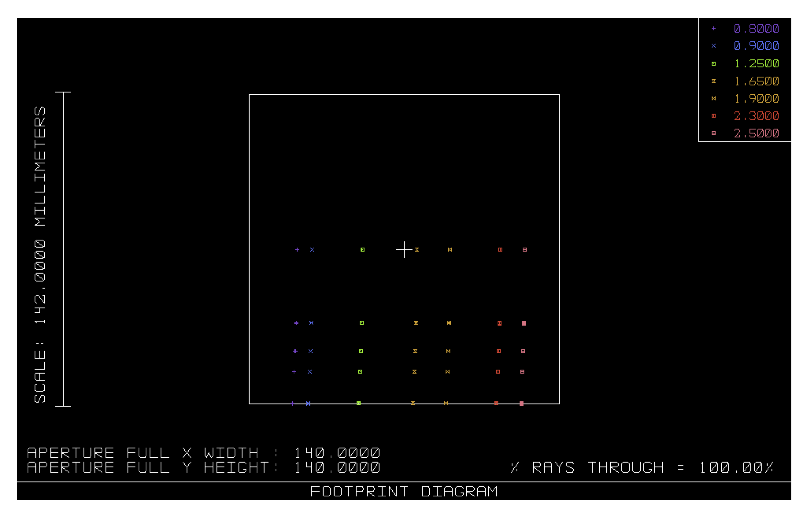
\includegraphics[width=120mm]{\thisdir figs/optcraft_fig06.eps}
}
\caption{Spectroscopic image positions for a configuration shown in Fig.~\ref{fig:optcraft_fig01}.
}
\label{fig:optcraft_fig06}
\end{figure}

\begin{figure}[!ht]
\centerline{
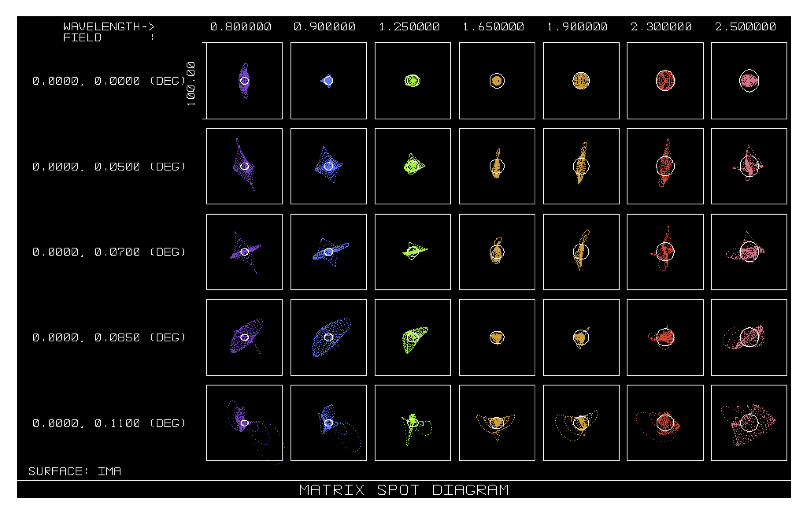
\includegraphics[width=120mm]{\thisdir figs/optcraft_fig07.eps}
}
\caption{Spot diagram for spectroscopy with a configuration shown in
 Fig.~\ref{fig:optcraft_fig01}.}
\label{fig:optcraft_fig07}
\end{figure}

Next we examined the case where there is no change in the telescope
parameters again, and a field flatner which consists of two lenses. 
Fig.~\ref{fig:optcraft_fig08} shows the optical layout of the case.

\begin{figure}[!ht]
\centerline{
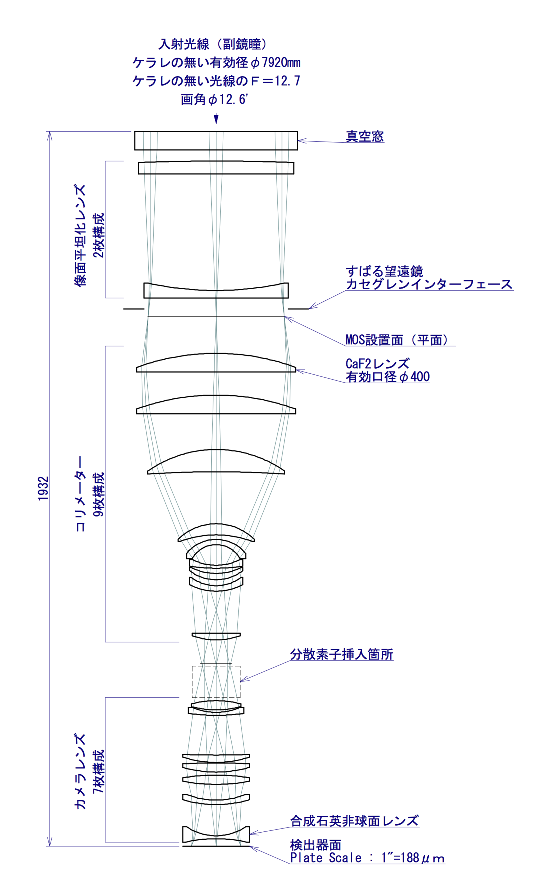
\includegraphics[width=120mm]{\thisdir figs/optcraft_fig08.eps}
}
\caption{Optical layout for Case A: no change in the telescope
 parameters. The case with field flatner.
}
\label{fig:optcraft_fig08}
\end{figure}

The optical design was made so that the effective diameter of the
largest lens is no larger than $\phi$400mm, as it is in the case without
the flatner. The field of view is $\phi 12.6'$, which is slightly
smaller than the case without the flatner, because the field flatner
acts like a concave lens and we need collimator lenses larger than the
flatner. The effective diameter of the primary mirror to block the light
outside of the primary mirror is $\phi$7.92m.
In addition to make the telescope focal plane flat, the addition of the
flatner enables a correction of astigmatism. As shown in 
Fig.~\ref{fig:optcraft_fig09}, the image quality is good at the flat MOS
mask, and there is no chromatic abberation.
We should note that there is distortion, which amounts +0.73\% at the
edge of the FoV.

\begin{figure}[!ht]
\centerline{
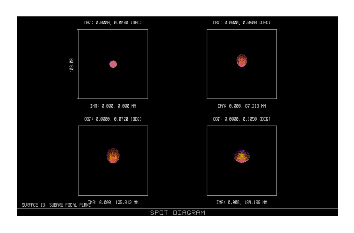
\includegraphics[width=100mm]{\thisdir figs/optcraft_fig09.eps}
 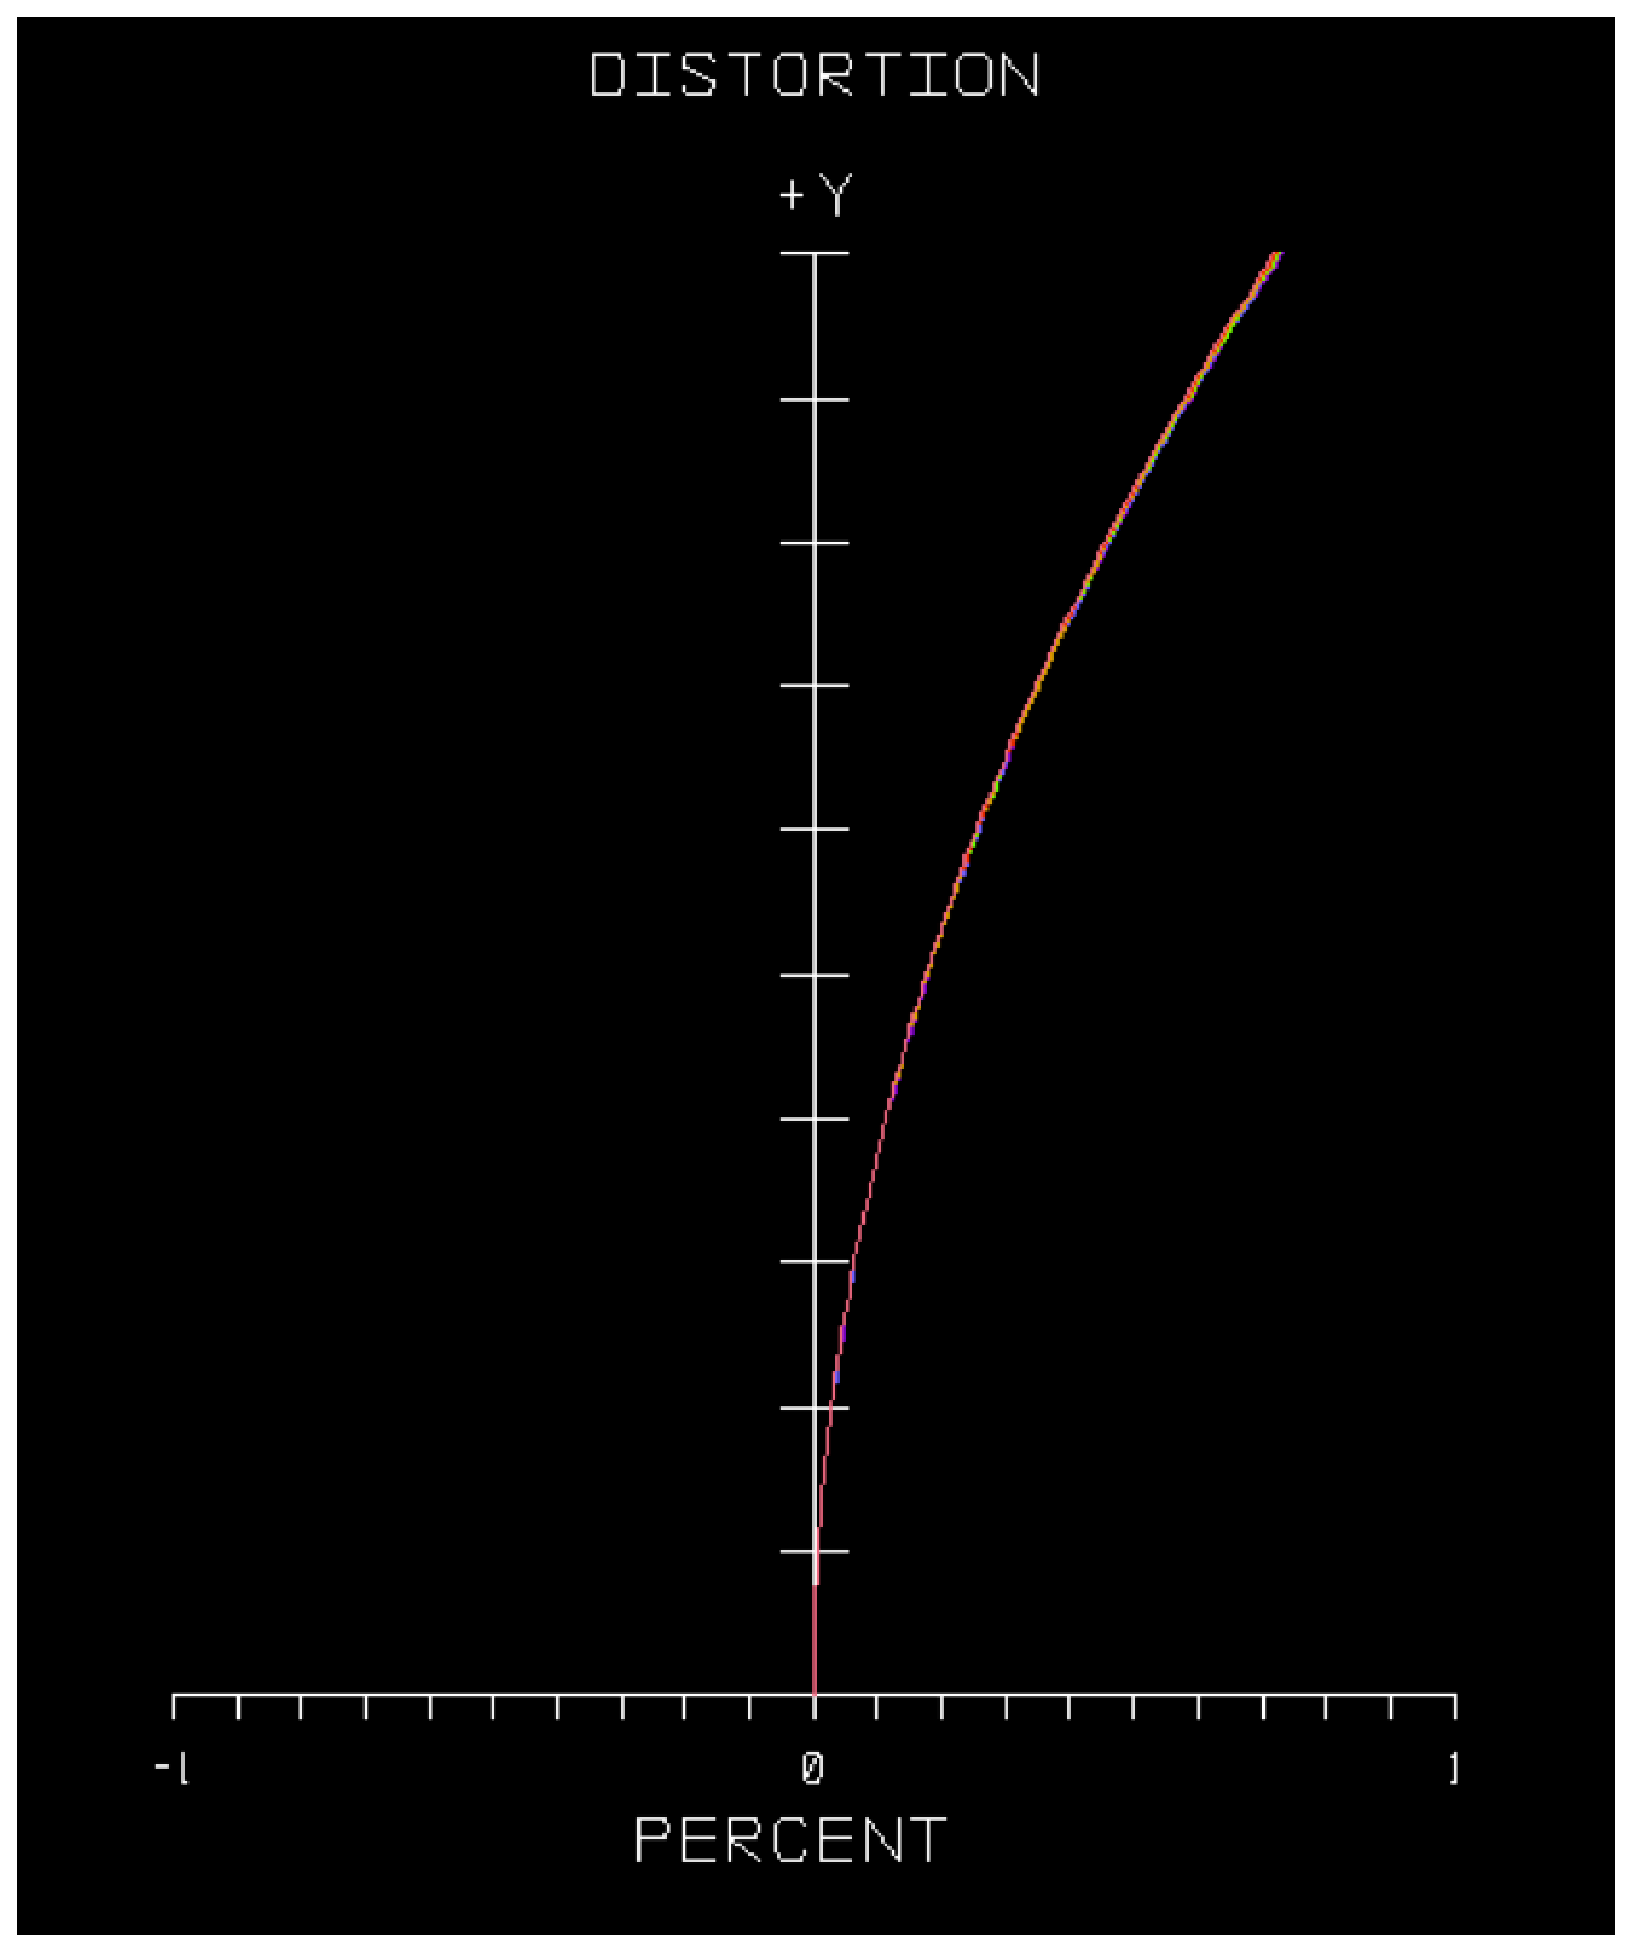
\includegraphics[width=60mm]{\thisdir figs/optcraft_fig10.eps}
}
\caption{(Left) Spot diagram at the MOS mask plate.
(Right) distortion at the MOS mask plate.
}
\label{fig:optcraft_fig09}
\end{figure}

For the image quality at the position of the detectors, similar to the
case without the flatner, in the most of the FoV and for the most of the
wavelength range the image quality satisfies the goal (FWHM smaller than
approx. $0.15''$), while in a few cases (such at the FoV edge ($6.3'$
from the center) and with 0.8$\mu$m) the image quality is slightly worse
than the goal. Distortion is large; it is $-5.2$\% at the edge of FoV.
Performance in the spectroscopy is also similar to the case without the
flatner, and in most cases the qulality satisfies the goal.
We should note that with the field flatner the optical layout is not
telecentric, and the plate scale should be changed if there is a focus
offset.  So the focusing is more important in this case.




\subsubsection{B. Cases in which Subaru Telescope optical parameters are
   changed}

Next we examined the case in which Subaru Telescope's optical parameters
are changed. In order to make the telescope's F number smaller, the
primary mirror's aspheric parameters should be negative. The actuator
storoke for the primary mirror is guaranteed up to 12$\mu$m. We assume
the conic parameters so that displacement at the edge of the primary
mirror is 12$\mu$m, and set F number to be 9.8.

The parameters of the secondary mirror is determined as it is optimal
for this Cassegrain wide-field instrument, and it is independent from
the existing secondary mirrors of Subaru Telescope.
It is a bipolar mirror with a diameter of $\phi$1544mm. The radius of
curvature is 7233.308mm and the conic constant is $-2.35464$.
The field of view is determined by the effective maximum size of the
lens ($\phi$400mm), and it is $\phi16.2'$.
Thanks to the smaller F number, the field of view is 28\% larger than
the case without changing the telescope parameters. The effective
diameter of the primary mirror to avoid the beam outside of the
secondary pupil and primary mirror ($\phi$8.2m) is $\phi$7.93m.

\begin{figure}[!ht]
\centerline{
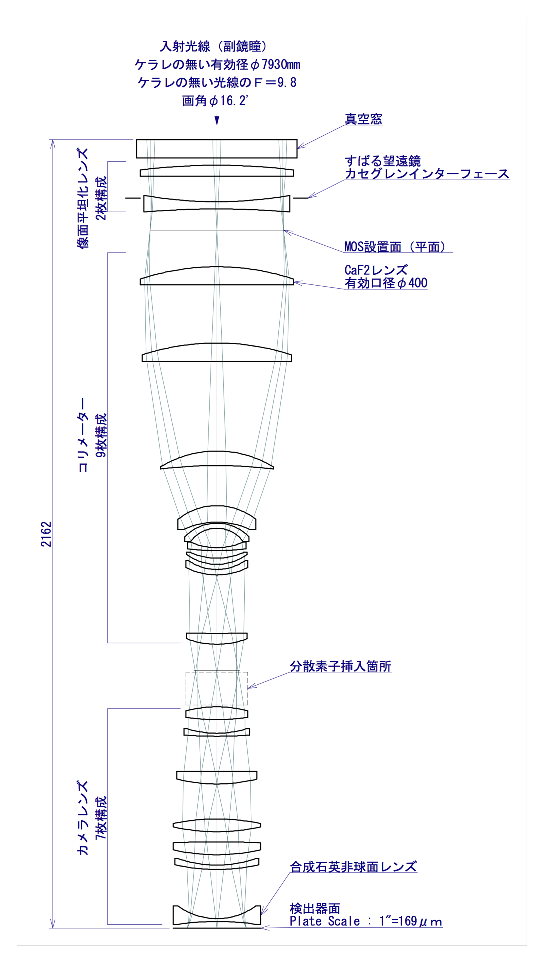
\includegraphics[width=120mm]{\thisdir figs/optcraft_fig15.eps}
}
\caption{The optical layout of the case B: Subaru Telescope
 optical parameters are modified. A field flatner is included in this
 design. 
}
\label{fig:optcraft_fig15}
\end{figure}

In this design a set of lenses as a field flatner is included. 
The spot diagram at the flat MOS mask position is presented in 
Fig. \ref{fig:optcraft_fig16}.
Although small coma aberration is present, its effect is small. There is
no chromatic aberration, overall image quality is good, although there
is distortion aberration at the edge of the FoV.

\begin{figure}[!ht]
\centerline{
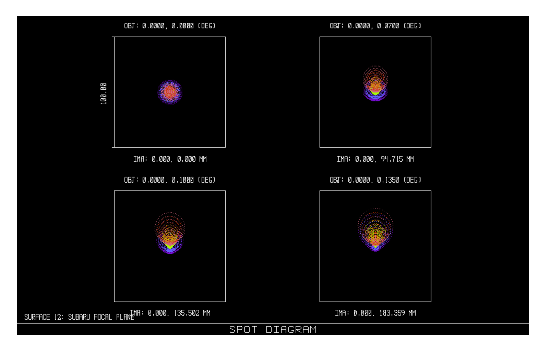
\includegraphics[width=100mm]{\thisdir figs/optcraft_fig16.eps}
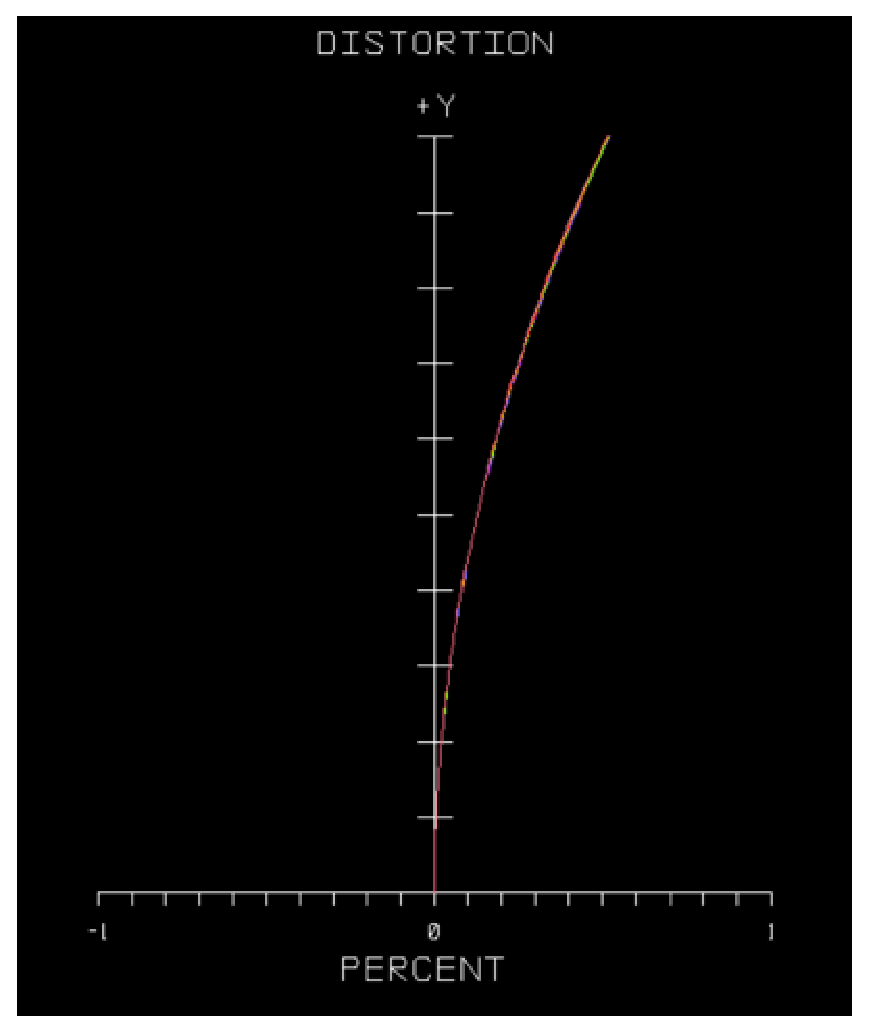
\includegraphics[width=60mm]{\thisdir figs/optcraft_fig17.eps}
}
\caption{(Left) Spot diagram at the MOS mask position.
(Right) distortion aberration at the MOS mask position.
}
\label{fig:optcraft_fig16}
\end{figure}

The configuration of optics after MOS position is similar to the case
without change of the telescope parameters: collimator with nine lenses
and camera with seven lenses. The focal plane is flat. The optical
layout in shown in Fig.\ref{fig:optcraft_fig15}.

In Fig. \ref{fig:optcraft_fig18} we show the spot diagram and distortion
aberration at the position of detectors.
Image quality at outskirt of the FoV ($>6'$) in a short wavelength
(0.8--0.9$\mu$m) degrades by $\sim0.2''$. Otherwise image quality
satisfies the goal (FWHM$\sim 0.15''$).
The maximum distortion aberration at the edge of FoV is $-1.24$\%, which
is smaller than the cases without changes in telescope parameters.

\begin{figure}[!ht]
\centerline{
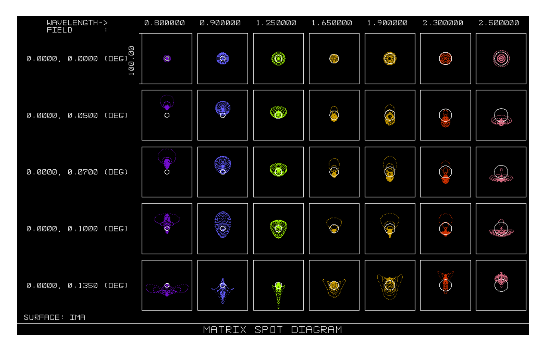
\includegraphics[width=120mm]{\thisdir figs/optcraft_fig18.eps}
\includegraphics[width=60mm]{\thisdir figs/optcraft_fig19.eps}
}
\caption{(Left) Spot diagram at the positions of the detectors.
Images with five positions within the FoV (vertical) and seven
 wavelengths from 0.8$\mu$m to 2.5$\mu$m (horizontal) are plotted.
The box size is 100$\mu$m, which corresponds to $0.59''$.
The RMS spot diameters are $0.2''$ (at $8.1'$, $0.8\mu$m), 
$0.16''$ (at $6'$, $0.8\mu$m), $0.19''$ (at $6'$, $0.9\mu$m), and for
 other positions and wavelength the spot diameters are within $0.15''$.
(Right) Distortion aberration. It reaches to $-1.24$\% at the edge of
 the FoV.
}
\label{fig:optcraft_fig18}
\end{figure}

Performance in spectroscopy mode is examined and is reported in 
Fig.~\ref{fig:optcraft_fig20}. Here a grism made of fused silica, 160
lines/mm, blaze angle 35$^\circ$ is assumed, and the sizes of spectra on
the detector is presented.

In regards to the image quality, as shown in
Fig.~\ref{fig:optcraft_fig21}, in some cases at the edge of FoV or
shortest/longest wavelengths the RMS spot diameter becomes as large as 
$0.23''$. Otherwise the image quality satisfies the goal, especially
within $6'$ from the center of FoV.

\begin{figure}[!ht]
\centerline{
\includegraphics[width=120mm]{\thisdir figs/optcraft_fig20.eps}
}
\caption{
Spectroscopic image positions for a configuration shown in
 Fig.~\ref{fig:optcraft_fig15}. The box size is 180mm. We assume to use
 a grism made of fused silica with 160 lines/mm, and blaze angle
 35$^\circ$.
}
\label{fig:optcraft_fig20}
\end{figure}

\begin{figure}[!ht]
\centerline{
\includegraphics[width=120mm]{\thisdir figs/optcraft_fig21.eps}
}
\caption{Spot diagram for Case B, spectroscopy mode.
In shorter wavelength the performance is somewhat worse than the goal;
 at 0.8$\mu$m RMS spot diameters are in general 0.17--0.18$''$, and 
 0.2$''$ at 0.9$\mu$m. In longer wavelength spot diameter becomes larger
 at positions with distance from the center larger than $6'$ with
 $\lambda = 2.3-2.5\mu$m. Otherwise the image quality satisfies the goal
 ($0.15''$).
}
\label{fig:optcraft_fig21}
\end{figure}



\subsection{Optical Design with FoV Split}

\subsubsection{Case A: secondary mirror parameter is the same as
   existing one}

\subsubsection{Case B: secondary mirror parameter is modified}



%%% 20130906 iwata

\section{Optical Design Concept of Wide-field Imager for GLAO}

Proposed by J. Pazder (NRC-NSI-AST / HIA)

\bigskip

\section{Multi Integral-Field-Unit Instrument}

Describe overview of KMOS, discuss feasibility of Multi-IFU instrument
at the Cassegrain focus.

\bigskip

\section{Technical Issues of Wide-field NIR instrument}

\subsection{Mask Exchange Mechanism for MOS}

\subsection{Narrow-band Filters}

\subsection{Size and weight}


%%% Development Plan
\include{project/hayano/development_plan}

\include{project/actions/action_items}

\end{document}
